%------------------------------------------------------------------------
%- Reference for the EALib, package Rng                                 -
%------------------------------------------------------------------------
%- History of modification                                              -
%-                                                                      -
%-  ver.1.01 : 2000/05/29 Ruediger Alberts (Institut fuer               -
%-                        Neuroinformatik, Bochum)                      -
%-               original                                               -
%-  ver.1.02 : 2001/01/04 Tatsuya Okabe (HONDA R&D EUROPE DEUTSCHLAND)  -
%-               separate files , add index                             -
%-  ver.1.03 : 2001/01/30 Tatsuya Okabe (HONDA R&D EUROPE DEUTSCHLAND)  -
%-               include some classes about random generator            -
%-  ver.1.04 : 2001/02/05 Tatsuya Okabe (HONDA R&D EUROPE DEUTSCHLAND)  -
%-               include some important classes                         -
%-  ver.1.10 : 2001/02/14 Tatsuya Okabe (HONDA R&D EUROPE DEUTSCHLAND)  -
%-               release version                                        -
%-  ver.1.11 : 2001/06/08 Tatsuya Okabe (HONDA R&D EUROPE DEUTSCHLAND)  -
%-               correct some mistakes                                  -
%-  ver.1.12 : 2002/05/22 Ruediger Alberts (ZN AG, Bochum)              -
%-               splitted parts for EALib, Array and Rng                -
%-                                                                      -
%-  ver.1.13 :                                                          -
%-                                                                      -
%-  ver.1.14 :                                                          -
%-                                                                      -
%-  ver.1.15 :                                                          -
%-                                                                      -
%------------------------------------------------------------------------

\documentclass{report}
\usepackage{a4}
\usepackage{graphicx}
\usepackage{makeidx}
\makeindex
% =======================================================================
% Dateiname:        Vorlage.tex
% Autor:            Ruediger Alberts
% EMail:            Ruediger.Alberts@neuroinformatik.ruhr-uni-bochum.de
% Erstellt am:      1999-09-07
% Letzte Aenderung: 1999-09-09
%
% Datei wird mit Befehl ``% =======================================================================
% Dateiname:        Vorlage.tex
% Autor:            Ruediger Alberts
% EMail:            Ruediger.Alberts@neuroinformatik.ruhr-uni-bochum.de
% Erstellt am:      1999-09-07
% Letzte Aenderung: 1999-09-09
%
% Datei wird mit Befehl ``% =======================================================================
% Dateiname:        Vorlage.tex
% Autor:            Ruediger Alberts
% EMail:            Ruediger.Alberts@neuroinformatik.ruhr-uni-bochum.de
% Erstellt am:      1999-09-07
% Letzte Aenderung: 1999-09-09
%
% Datei wird mit Befehl ``\input{Vorlage}'' in LaTex-Dokumente 
% (Latex2Epsilon) eingebunden und stellt Befehle zur einfachen Doku- 
% mentation von C-Funktionen/C++-Methoden bereit.
% =======================================================================

\usepackage{ifthen}

    % Definition von Konstanten:
    \newcommand{\ParamDelim}            % Trennungstext zwischen
        { \ - }                         % Parametername und -beschreibung.
    \newcommand{\NormMethodEnd}         % Endtext von Methode bei 
        {\ \ );}                        % veraenderbarer Aufrufinstanz.
    \newcommand{\ConstMethodEnd}        % Endtext von Methode bei
        {\ \ ) const;}                  % nicht veraenderbarer Aufrufinstanz.
    \newcommand{\MaxLabelTxt}           % Komponentenbeschreibungstext
        {{\bf Besonderheiten: }}        % mit maximaler Breite.
    \newcommand{\MethodBegin}           % Beginntext einer Methode.
        {(\ }
    \newcommand{\InBetween}             % Text zwischen Rueckgabewert und
        {\ \ }                          % Methodenname.

    % Definition eigener Variablen:


    \newboolean{ConstInstance}          % Gibt an, ob die Instanz, die
                                        % die Methode aufruft veraendert
                                        % werden darf oder nicht. Im
                                        % 2. Fall endet die Methode mit
                                        % ``) const;'', im 1. Fall 
                                        % mit ``);''.
    \newcounter{SavedParams}            % Anzahl der gespeicherten
                                        % Parameter.
    \setcounter{SavedParams}{0}
    \newcommand{\ParamOne}{}            % Definition der 10 
    \newcommand{\ParamTypeOne}{}        % abspeicherbaren Parameter,
    \newcommand{\ParamDescrOne}{}       % ihrer Typen und Beschreibungen.
    \newcommand{\ParamTwo}{}            
    \newcommand{\ParamTypeTwo}{}
    \newcommand{\ParamDescrTwo}{}
    \newcommand{\ParamThree}{}
    \newcommand{\ParamTypeThree}{}
    \newcommand{\ParamDescrThree}{}
    \newcommand{\ParamFour}{}
    \newcommand{\ParamTypeFour}{}
    \newcommand{\ParamDescrFour}{}
    \newcommand{\ParamFive}{}
    \newcommand{\ParamTypeFive}{}
    \newcommand{\ParamDescrFive}{}
    \newcommand{\ParamSix}{}
    \newcommand{\ParamTypeSix}{}
    \newcommand{\ParamDescrSix}{}
    \newcommand{\ParamSeven}{}
    \newcommand{\ParamTypeSeven}{}
    \newcommand{\ParamDescrSeven}{}
    \newcommand{\ParamEight}{}
    \newcommand{\ParamTypeEight}{}
    \newcommand{\ParamDescrEight}{}
    \newcommand{\ParamNine}{}
    \newcommand{\ParamTypeNine}{}
    \newcommand{\ParamDescrNine}{}
    \newcommand{\ParamTen}{}
    \newcommand{\ParamTypeTen}{}
    \newcommand{\ParamDescrTen}{}
    \newlength{\MaxParamWidth}          % Breite des breitesten 
                                        % Methodenparameters.
    \newlength{\SpecialWidth}           % Breite des Textes 
    \settowidth{\SpecialWidth}          % {\bf Besonderheiten}.
        {\MaxLabelTxt}
    \newlength{\ParamDelimWidth}        % Breite des Textes `` \ - ``.
    \settowidth{\ParamDelimWidth}
        {\ParamDelim}
    \newlength{\ParamDescrWidth}        % Max. Breite des Parametertextes.
    \newlength{\SpecialRetTxtWidth}     % Max. Breite der Texte fuer
                                        % Besonderheiten und Rueckgabewert.
    \newlength{\MethodBeginWidth}       % Breite des Methodenanfangs, d.h.
                                        % ``Rueckgabewert Methodenname ( ``.
    \newlength{\BetweenParsWidth}       % Max. zur Verfuegung stehende
                                        % Breite zwischen den beiden Klammern
                                        % der Methode.
    
    \newlength{\MethodEndWidth}         % Breite des Textes ``  );'' bzw.
    \settowidth{\MethodEndWidth}        % `` ) const;''
        {\NormMethodEnd}
    \newlength{\ParamMaxTypeWidth}      % Breite des breitesten
                                        % Parameterwert-Typs. 
    \newlength{\NoneWidthOne}           % Breite des Textes ``Keine.''.
    \settowidth{\NoneWidthOne}{Keine.}
    \newlength{\NoneWidthTwo}           % Breite des Textes ``Keiner.''.
    \settowidth{\NoneWidthTwo}{Keiner.}
    \newlength{\Temp}                   % Temporaere Hilfsvariable. 
    \newlength{\VertSpace}              % Vertikaler Abstand zwischen 
                                        % zwei Parboxen.
   
    % Trotz der automatischen Berechnung der Textbreiten treten
    % kleine Unstimmigkeiten von wenigen Punkten bei den Texten
    % zur Beschreibung der Parameter, des Rueckgabewertes und
    % der Besonderheiten auf, die mit den folgenden Variablen
    % behoben werden koennen:

    \newlength{\CorrectWidthOne}        % Korrekturbreite fuer die
                                        % Parameterbeschreibung.
    \newlength{\CorrectWidthTwo}        % Korrekturbreite fuer die
                                        % Beschreibungen von Rueckgabewert
                                        % und Besonderheiten.
    \newlength{\CorrectWidthThree}      % Korrekturbreite, da erster
                                        % Parameter einer Methode weiter
                                        % vorrueckt als die anderen.
    

% Uebersicht ueber die Parameter und ihre Bedeutung.


%
% <-- \MethodBeginWidth    -->
%------------------------------------------------------------------------
% Rueckgabewert Methodenname(   Typ_Parameter_1 Parameter_1,
%                            <->Typ_Parameter_2 Parameter_2,
%              \CorrectWideThree...
%                               Typ_Parameter_n Parameter_n   );
%                             <-------------> <--------->
%                          \ParamMaxTypeWidth \MaxParamWidth
%                             <-------------------------->
%                             \BetweenParsWidth
%                                                         <-->
%                                                         \MethodEndWidth
%------------------------------------------------------------------------
% Beschreibung der Methode...
%                             \ParamDelimWidth
%                             <->                        \CorrectWidthOne
% \VertSpace
% Parameter:       Parameter_1  - Beschreibung von Parameter 1.   <----->
%                  Parameter_2  - Beschreibung von Parameter 2.
%                  ...
%                  Parameter_n  - Beschreibung von Parameter n.
% \VertSpace                      \ParamDescrWidth
%                                 <------------------------------>
% Rueckgabewert:   Beschreibung des Rueckgabewertes bzw. der Text <-----> 
%                  Keiner.                   
%                  <----->
%                  \NoneWidthTwo               \SpecialRetTxtWidth
% \VertSpace       <--------------------------------------------->
% Besonderheiten:  Beschreibung von Besonderheiten bzw. der Text  <----->
%                  Keine.     
% <--------------> <---->
%  \SpecialWidth   \NoneWidthOne                         \CorrectWidthTwo


    % Definition eigener Befehle:


    %-----------------------------------------------------------------------
    % Gibt den Begriff ``C++'' in ansprechender Form aus.
    % Makro wurde freundlicherweise zur Verfuegung gestellt von
    % Axel W. Dietrich.
    %
    \newcommand{\cpp}{
        \mbox{\emph{\textrm{C\hspace{-1.5pt}\raisebox{1.75pt}{\scriptsize +}
        \hspace{-6pt}\raisebox{.75pt}{\scriptsize +}}}}%
    }


    %-----------------------------------------------------------------------
    % Gibt die Werte aller Parameter auf dem Bildschirm aus.
    %
    \newcommand{\showAllParams}{
        \noindent
        {\em Werte aller Parameter:}
        \begin{tabbing}
            ParamMaxTypeWidth:\ \ \=\kill
            MaxParamWidth:       \>\the\MaxParamWidth\\
            SpecialWidth:        \>\the\SpecialWidth\\
            ParamDelimWidth:     \>\the\ParamDelimWidth\\
            ParamDescrWidth:     \>\the\ParamDescrWidth\\
            SpecialRetTxtWidth:  \>\the\SpecialRetTxtWidth\\
            MethodBeginWidth:    \>\the\MethodBeginWidth\\
            BetweenParsWidth:    \>\the\BetweenParsWidth\\
            MethodEndWidth:      \>\the\MethodEndWidth\\
            ParamMaxTypeWidth:   \>\the\ParamMaxTypeWidth\\
            NoneWidthOne:        \>\the\NoneWidthOne\\
            NoneWidthTwo:        \>\the\NoneWidthTwo\\
            VertSpace:           \>\the\VertSpace\\
            CorrectWidthOne:     \>\the\CorrectWidthOne\\
            CorrectWidthTwo:     \>\the\CorrectWidthTwo\\
            CorrectWidthThree:   \>\the\CorrectWidthThree\\
            ConstInstance:       
            \ifthenelse{\boolean{ConstInstance}}
                {\>ja\\}
                {\>nein\\}
        \end{tabbing}
    }

    %-----------------------------------------------------------------------
    % Setzt einen Schalter, der angibt, dass die Instanz, die die kommende
    % Methode aufrufen kann, nicht veraendert werden darf. Dies hat fuer
    % die Dokumentation zur Folge, dass die Methode mit ``) const;'' endet.
    %
    \newcommand{\setConstInstance}{    
        \setboolean{ConstInstance}{true}
    }

    %-----------------------------------------------------------------------
    % Setzt einen Schalter, der angibt, dass die Instanz, die die kommende
    % Methode aufrufen kann, veraendert werden darf. Die Methode endet also
    % in der Dokumentation normal mit ``);''.
    %
    \newcommand{\setNormalInstance}{    
        \setboolean{ConstInstance}{false}
    }

    %-----------------------------------------------------------------------
    % Initialisiert die Breite des breitesten Methodenparametertyptextes
    % mit Null.
    %
    \newcommand{\initParamMaxTypeWidth}{
        \setlength{\ParamMaxTypeWidth}{0pt}
    }

    %-----------------------------------------------------------------------
    % Initialisiert die Breite des breitesten Parameternamens mit Null.
    %
    \newcommand{\initMaxParamWidth}{
        \setlength{\MaxParamWidth}{0pt}
    }

    %-----------------------------------------------------------------------
    % Ueberprueft, ob die Breite des uebergebenen Textes des Parametertyps
    % groesser ist als die des bisher als breitester Typtext festgelegten
    % Textes und passt den Wert evtl. an.
    % Parameter #1:  Neuer Typtext, dessen Breite zum Vergleich dient.
    %   
    \newcommand{\setNewParamMaxTypeWidth}[1]{
        \settowidth{\Temp}{#1}
        \ifthenelse{\lengthtest{\ParamMaxTypeWidth < \Temp}}
            {\setlength{\ParamMaxTypeWidth}{\Temp}}{}   
    }

    %-----------------------------------------------------------------------
    % Ueberprueft, ob die Breite des uebergebenen Parameternamens groesser
    % ist als die des bisher als am breitesten geltenden Parameternames
    % und passt den Wert evtl. an. Der Parametername steht dabei in
    % Emphasized.
    % Parameter #1:  Neuer Parametername, dessen Breite zum Vergleich dient.
    %
    \newcommand{\setNewMaxParamWidth}[1]{
        \settowidth{\Temp}{{\em #1}}
        \ifthenelse{\lengthtest{\MaxParamWidth < \Temp}}
            {\setlength{\MaxParamWidth}{\Temp}}{}
    }

    %-----------------------------------------------------------------------
    % Setzt die Breite der Beschreibungstexte fuer Rueckgabewert
    % und Besonderheiten.
    %
    \newcommand{\setSpecialRetTxtWidth}{
        \setlength{\SpecialRetTxtWidth}{\textwidth}
        \addtolength{\SpecialRetTxtWidth}{-1\SpecialWidth} 
    }

    %-----------------------------------------------------------------------
    % Setzt die Breite fuer den Beginn einer Methode, d.h. den Text
    % ``Rueckgabewert Methodenname( ``. Rueckgabewert steht dabei
    % in Emphasized, Methodenname in Bold Font.
    % Parameter #1:  Rueckgabewert der Methode.
    % Parameter #2:  Name der Methode.
    %
    \newcommand{\setMethodBeginWidth}[2]{
        \settowidth{\MethodBeginWidth}
            {{\em #1}\InBetween{\bf #2}\MethodBegin}
    }

    %-----------------------------------------------------------------------
    % Setzt die maximale Breite die an Platz zwischen der oeffnenden
    % und der schliessenden Klammer der Methode zur Verfuegung steht.
    %
    \newcommand{\setBetweenParsWidth}{
        \setlength{\BetweenParsWidth}{\textwidth}
        \addtolength{\BetweenParsWidth}{-1\MethodBeginWidth}
        \addtolength{\BetweenParsWidth}{-1\MethodEndWidth}
    }

    %-----------------------------------------------------------------------
    % Setzt die Breite fuer die Beschreibungstexte
    % der Methodenparameter.
    %
    \newcommand{\setParamDescrWidth}{
        \setlength{\ParamDescrWidth}{\textwidth}
        \addtolength{\ParamDescrWidth}{-1\SpecialWidth} 
        \addtolength{\ParamDescrWidth}{-1\MaxParamWidth}
        \addtolength{\ParamDescrWidth}{-1\ParamDelimWidth}
    }    

    %-----------------------------------------------------------------------
    % Setzt die Korrekturbreite fuer den Beschreibungstext von
    % Methodenparametern auf den uebergebenen Wert.
    % Parameter #1:  Neuer Wert fuer die Korrekturbreite.
    %
    \newcommand{\setCorrectWidthOne}[1]{
        \setlength{\CorrectWidthOne}{#1}
    }    

    %-----------------------------------------------------------------------
    % Setzt die Korrekturbreite fuer den Beschreibungstext von
    % Rueckgabewert und Besonderheiten auf den uebergebenen Wert.
    % Parameter #1:  Neuer Wert fuer die Korrekturbreite.
    %
    \newcommand{\setCorrectWidthTwo}[1]{
        \setlength{\CorrectWidthTwo}{#1}
    }    

    %-----------------------------------------------------------------------
    % Setzt die Korrekturbreite fuer den Abstand des zweiten bis n-ten
    % Parameters vom Anfang auf den uebergebenen Wert.
    % Parameter #1:  Neuer Wert fuer die Korrekturbreite.
    %
    \newcommand{\setCorrectWidthThree}[1]{
        \setlength{\CorrectWidthThree}{#1}
    }    

    %-----------------------------------------------------------------------
    % Setzt den vertikalen Abstand zwischen zwei Parboxen auf den ueber-
    % gebenen Wert.
    % Parameter #1:  Neuer Wert fuer den vertikalen Abstand.
    %
    \newcommand{\setVertSpace}[1]{
        \setlength{\VertSpace}{#1}
    }    

    %-----------------------------------------------------------------------
    % Speichert die uebergebenen Informationen ueber Methodenparameter 1
    % in internen Variablen. Achtung: Die Parameter muessen in der richtigen
    % Reihenfolge gesetzt werden!
    % Parameter #1: Der Typ des Parameters.  
    % Parameter #2: Der Name des Parameters. 
    % Parameter #3: Die Beschreibung des Parameters. 
    % 
    \newcommand{\setParamOne}[3]{
        \renewcommand{\ParamOne}{#1}
        \renewcommand{\ParamTypeOne}{#2}
        \renewcommand{\ParamDescrOne}{#3} 
        \setcounter{SavedParams}{0}
        \stepcounter{SavedParams}
    }

    %-----------------------------------------------------------------------
    % Speichert die uebergebenen Informationen ueber Methodenparameter 2
    % in internen Variablen. Achtung: Die Parameter muessen in der richtigen
    % Reihenfolge gesetzt werden!
    % Parameter #1: Der Typ des Parameters.  
    % Parameter #2: Der Name des Parameters. 
    % Parameter #3: Die Beschreibung des Parameters. 
    % 
    \newcommand{\setParamTwo}[3]{
        \renewcommand{\ParamTwo}{#1}
        \renewcommand{\ParamTypeTwo}{#2}
        \renewcommand{\ParamDescrTwo}{#3} 
        \stepcounter{SavedParams}
    }

    %-----------------------------------------------------------------------
    % Speichert die uebergebenen Informationen ueber Methodenparameter 3
    % in internen Variablen. Achtung: Die Parameter muessen in der richtigen
    % Reihenfolge gesetzt werden!
    % Parameter #1: Der Typ des Parameters.  
    % Parameter #2: Der Name des Parameters. 
    % Parameter #3: Die Beschreibung des Parameters. 
    % 
    \newcommand{\setParamThree}[3]{
        \renewcommand{\ParamThree}{#1}
        \renewcommand{\ParamTypeThree}{#2}
        \renewcommand{\ParamDescrThree}{#3} 
        \stepcounter{SavedParams}
    }

    %-----------------------------------------------------------------------
    % Speichert die uebergebenen Informationen ueber Methodenparameter 4
    % in internen Variablen. Achtung: Die Parameter muessen in der richtigen
    % Reihenfolge gesetzt werden!
    % Parameter #1: Der Typ des Parameters.  
    % Parameter #2: Der Name des Parameters. 
    % Parameter #3: Die Beschreibung des Parameters. 
    % 
    \newcommand{\setParamFour}[3]{
        \renewcommand{\ParamFour}{#1}
        \renewcommand{\ParamTypeFour}{#2}
        \renewcommand{\ParamDescrFour}{#3} 
        \stepcounter{SavedParams}
    }

    %-----------------------------------------------------------------------
    % Speichert die uebergebenen Informationen ueber Methodenparameter 5
    % in internen Variablen. Achtung: Die Parameter muessen in der richtigen
    % Reihenfolge gesetzt werden!
    % Parameter #1: Der Typ des Parameters.  
    % Parameter #2: Der Name des Parameters. 
    % Parameter #3: Die Beschreibung des Parameters. 
    % 
    \newcommand{\setParamFive}[3]{
        \renewcommand{\ParamFive}{#1}
        \renewcommand{\ParamTypeFive}{#2}
        \renewcommand{\ParamDescrFive}{#3} 
        \stepcounter{SavedParams}
    }

    %-----------------------------------------------------------------------
    % Speichert die uebergebenen Informationen ueber Methodenparameter 6
    % in internen Variablen. Achtung: Die Parameter muessen in der richtigen
    % Reihenfolge gesetzt werden!
    % Parameter #1: Der Typ des Parameters.  
    % Parameter #2: Der Name des Parameters. 
    % Parameter #3: Die Beschreibung des Parameters. 
    %     
    \newcommand{\setParamSix}[3]{
        \renewcommand{\ParamSix}{#1}
        \renewcommand{\ParamTypeSix}{#2}
        \renewcommand{\ParamDescrSix}{#3} 
        \stepcounter{SavedParams} 
    }

    %-----------------------------------------------------------------------
    % Speichert die uebergebenen Informationen ueber Methodenparameter 7
    % in internen Variablen. Achtung: Die Parameter muessen in der richtigen
    % Reihenfolge gesetzt werden!
    % Parameter #1: Der Typ des Parameters.  
    % Parameter #2: Der Name des Parameters. 
    % Parameter #3: Die Beschreibung des Parameters. 
    %    
    \newcommand{\setParamSeven}[3]{
        \renewcommand{\ParamSeven}{#1}
        \renewcommand{\ParamTypeSeven}{#2}
        \renewcommand{\ParamDescrSeven}{#3} 
        \stepcounter{SavedParams} 
    }

    %-----------------------------------------------------------------------
    % Speichert die uebergebenen Informationen ueber Methodenparameter 8
    % in internen Variablen. Achtung: Die Parameter muessen in der richtigen
    % Reihenfolge gesetzt werden!
    % Parameter #1: Der Typ des Parameters.  
    % Parameter #2: Der Name des Parameters. 
    % Parameter #3: Die Beschreibung des Parameters. 
    % 
    \newcommand{\setParamEight}[3]{
        \renewcommand{\ParamEight}{#1}
        \renewcommand{\ParamTypeEight}{#2}
        \renewcommand{\ParamDescrEight}{#3} 
        \stepcounter{SavedParams}
    }

    %-----------------------------------------------------------------------
    % Speichert die uebergebenen Informationen ueber Methodenparameter 9
    % in internen Variablen. Achtung: Die Parameter muessen in der richtigen
    % Reihenfolge gesetzt werden!
    % Parameter #1: Der Typ des Parameters.  
    % Parameter #2: Der Name des Parameters. 
    % Parameter #3: Die Beschreibung des Parameters. 
    % 
    \newcommand{\setParamNine}[3]{
        \renewcommand{\ParamNine}{#1}
        \renewcommand{\ParamTypeNine}{#2}
        \renewcommand{\ParamDescrNine}{#3}  
        \stepcounter{SavedParams}
    }

    %-----------------------------------------------------------------------
    % Speichert die uebergebenen Informationen ueber Methodenparameter 10
    % in internen Variablen. Achtung: Die Parameter muessen in der richtigen
    % Reihenfolge gesetzt werden!
    % Parameter #1: Der Typ des Parameters.  
    % Parameter #2: Der Name des Parameters. 
    % Parameter #3: Die Beschreibung des Parameters. 
    % 
    \newcommand{\setParamTen}[3]{
        \renewcommand{\ParamTen}{#1}
        \renewcommand{\ParamTypeTen}{#2}
        \renewcommand{\ParamDescrTen}{#3} 
        \stepcounter{SavedParams}
    }

    %-----------------------------------------------------------------------
    % Gibt den Text ``Rueckgabewert Methodenname(`` aus.
    % Parameter #1:  Rueckgabewert der Methode.
    % Parameter #2:  Name der Methode.
    %
    \newcommand{\printMethodBegin}[2]{
         \ifthenelse{\boolean{ConstInstance}}
             {\settowidth{\MethodEndWidth}{\ConstMethodEnd}}
             {\settowidth{\MethodEndWidth}{\NormMethodEnd}}
         \setMethodBeginWidth{#1}{#2}
         \setBetweenParsWidth
         \noindent
         \hrulefill\\
         \noindent
         \parbox[t]{\MethodBeginWidth}
             {#1\InBetween{\bf #2}\MethodBegin}
     }

    %-----------------------------------------------------------------------
    % Gibt das Ende einer Methode aus, d.h. ``\ );'' oder ``\ ) const;''.
    %
    \newcommand{\printMethodEnd}{
        \ifthenelse{\boolean{ConstInstance}}
            {\ConstMethodEnd\\}
            {\NormMethodEnd\\}
            \mbox{}\hrulefill\\
    }

    %-----------------------------------------------------------------------
    % Gibt den Typen und Namen des einzigen Parameters einer Methode
    % gefolgt von dem Text ``  );'' bzw. `` ) const;'' aus.
    % Parameter #1:  Typ des Parameters.
    % Parameter #2:  Name des Parameters.
    % 
    \newcommand{\printMethodOneParam}[2]{
        \parbox[t]{\ParamMaxTypeWidth}{#1}
        \parbox[t]{\MaxParamWidth}{{\em #2}}
        \printMethodEnd
    }

    %-----------------------------------------------------------------------
    % Gibt den Typen und den Namen des ersten Methodenparameters aus.
    % Parameter #1:  Typ des Parameters.
    % Parameter #2:  Name des Parameters.
    %
    \newcommand{\printMethodFirstParam}[2]{
        \noindent
        \parbox[t]{\ParamMaxTypeWidth}{#1}
        \parbox[t]{\MaxParamWidth}{{\em #2},}\\[\VertSpace]
    }

    %-----------------------------------------------------------------------
    % Gibt den Typen und Namen des letzten Parameters einer Methode aus.
    % Parameter #1: Typ des Parameters.
    % Parameter #2: Name des Parameters.
    %
    \newcommand{\printMethodLastParam}[2]{
        \parbox[t]{\MethodBeginWidth}{\hfill}
        \hspace{\CorrectWidthThree}
        \parbox[t]{\ParamMaxTypeWidth}{#1}
        \parbox[t]{\MaxParamWidth}{{\em #2}}
        \printMethodEnd
    }

    %-----------------------------------------------------------------------
    % Gibt den Typen und Namen eines Methodenparameters aus.
    % Parameter #1:  Typ des Parameters.
    % Parameter #2: Name des Parameters.
    % Achtung: Nicht fuer den ersten oder letzten Parameter der Methode
    % geeignet!
    %
    \newcommand{\printMethodParam}[2]{
        \parbox[t]{\MethodBeginWidth}{\hfill}
        \hspace{\CorrectWidthThree}
        \parbox[t]{\ParamMaxTypeWidth}{#1}
        \parbox[t]{\MaxParamWidth}{{\em #2},}\\[\VertSpace]
    }

    %-----------------------------------------------------------------------
    % Gibt die Beschreibung einer Methode aus.
    % Parameter #1: Beschreibung der Methode.
    %
    \newcommand{\printMethodDescr}[1]{
        \newline
        \noindent
        #1\\[\VertSpace]
    }

    %-----------------------------------------------------------------------
    % Gibt den Text ``Parameter:    `` und danach den Namen des
    % ersten Parameters der Methode, gefolgt von seiner Beschreibung
    % aus.
    % Parameter #1:  Name des Parameters. 
    % Parameter #2:  Beschreibung des Parameters.
    %
    \newcommand{\printFirstParam}[2]{
        \setlength{\Temp}{\ParamDescrWidth}
        \addtolength{\Temp}{1\CorrectWidthOne}
        \parbox[t]{\SpecialWidth}{{\bf Parameter:}}
        \parbox[t]{\MaxParamWidth}{\em #1}
        \parbox[t]{\ParamDelimWidth}{\ParamDelim}
        \parbox[t]{\Temp}{#2}\\[\VertSpace]
    }

    %-----------------------------------------------------------------------
    % Gibt einen Parameter der Methode und die dazugehoerige Beschreibung
    % aus.
    % Parameter #1:  Name des Parameters.
    % Parameter #2:  Beschreibung des Parameters.
    %
    \newcommand{\printParam}[2]{
        \setlength{\Temp}{\ParamDescrWidth}
        \addtolength{\Temp}{1\CorrectWidthOne}
        \parbox[t]{\SpecialWidth}{\hfill}
        \parbox[t]{\MaxParamWidth}{\em #1}
        \parbox[t]{\ParamDelimWidth}{\ParamDelim}
        \parbox[t]{\Temp}{#2}\\[\VertSpace]
    }

    %-----------------------------------------------------------------------
    %
    % Gibt den Text ``Rueckgabewert:  `` gefolgt von einer Beschreibung
    % des Rueckgabewertes aus.
    % Parameter #1:  Beschreibung des Rueckgabewertes.
    %
    \newcommand{\printReturn}[1]{
        \setlength{\Temp}{\SpecialRetTxtWidth}
        \addtolength{\Temp}{1\CorrectWidthTwo}
        \parbox[t]{\SpecialWidth}{{\bf R\"uckgabewert:}}
        \parbox[t]{\Temp}{#1}\\[\VertSpace]
    }

    %-----------------------------------------------------------------------
    % Gibt den Text ``Besonderheiten:  `` gefolgt von einer Beschreibung
    % der Besonderheiten aus.
    % Parameter #1:  Beschreibung der Besonderheiten.
    %
    \newcommand{\printSpecial}[1]{
        \setlength{\Temp}{\SpecialRetTxtWidth}
        \addtolength{\Temp}{1\CorrectWidthTwo}
        \parbox[t]{\SpecialWidth}{\MaxLabelTxt}
        \parbox[t]{\Temp}{#1}\\[\VertSpace]
    }

    %-----------------------------------------------------------------------
    % Gibt den Text ``Parameter:        Keine.'' aus.
    %
    \newcommand{\printNoParams}{
        \parbox[t]{\SpecialWidth}{{\bf Parameter:}}
        \parbox[t]{\NoneWidthOne}{Keine.}\\[\VertSpace]
    }

    %-----------------------------------------------------------------------
    % Gibt den Text ``Rueckgabewert:  Keiner.'' aus.
    %
    \newcommand{\printNoReturn}{
        \parbox[t]{\SpecialWidth}{{\bf R\"uckgabewert:}}
        \parbox[t]{\NoneWidthTwo}{Keiner.}\\[\VertSpace]
    }

    %-----------------------------------------------------------------------
    % Gibt den Text ``Besonderheiten:  Keine.'' aus.
    %
    \newcommand{\printNoSpecial}{
        \parbox[t]{\SpecialWidth}{\MaxLabelTxt}
        \parbox[t]{\NoneWidthOne}{Keine.}\\[\VertSpace]
    }

    %-----------------------------------------------------------------------
    % Gibt den Text:
    % ``Parameter:       Keine.
    %   Rueckgabewert:   Keiner.
    %   Besonderheiten:  Keine.''
    % aus.
    %
    \newcommand{\printNoAll}{
        \printNoParams
        \printNoReturn
        \printNoSpecial
    }

    %-----------------------------------------------------------------------
    % Gibt eine Methode ohne Parameter, Rueckgabewert und Besonderheiten
    % aus.
    % Parameter #1:  Name der Methode.
    % Parameter #2:  Beschreibung der Methode.
    %
    \newcommand{\printEmptyMethod}[2]{
        \setSpecialRetTxtWidth
        \printMethodBegin{void}{#1}
        \printMethodEnd
        \printMethodDescr{#2}
        \printNoAll
    }

    %-----------------------------------------------------------------------
    % Gibt eine Methode ohne Parameter und Besonderheiten, aber mit
    % Rueckgabewert aus.
    % Parameter #1:  Rueckgabewert der Methode.
    % Parameter #2:  Name der Methode.
    % Parameter #3:  Beschreibung der Methode.
    % Parameter #4:  Beschreibung des Rueckgabewertes der Methode.
    %
    \newcommand{\printEmptyMethodReturn}[4]{
        \setSpecialRetTxtWidth
        \printMethodBegin{#1}{#2}
        \printMethodEnd
        \printMethodDescr{#3}
        \printNoParams
        \printReturn{#4}
        \printNoSpecial
    }

    %-----------------------------------------------------------------------
    % Gibt eine Methode ohne Parameter und Rueckgabewert, aber mit
    % Besonderheiten aus.
    % Parameter #1:  Name der Methode.
    % Parameter #2:  Beschreibung der Methode.
    % Parameter #3:  Beschreibung der Besonderheiten der Methode.
    %
    \newcommand{\printEmptyMethodSpecial}[3]{
        \setSpecialRetTxtWidth
        \printMethodBegin{void}{#1}
        \printMethodEnd
        \printMethodDescr{#2}
        \printNoParams
        \printNoReturn
        \printSpecial{#3}
    }

    %-----------------------------------------------------------------------
    % Gibt eine Methode ohne Parameter, aber mit Rueckgabewert
    % und Besonderheiten aus.
    % Parameter #1:  Rueckgabewert der Methode.
    % Parameter #2:  Name der Methode.
    % Parameter #3:  Beschreibung der Methode.
    % Parameter #4:  Beschreibung des Rueckgabewertes der Methode.
    % Parameter #5:  Beschreibung der Besonderheiten der Methode.
    %
    \newcommand{\printEmptyMethodReturnSpecial}[5]{
        \setSpecialRetTxtWidth
        \printMethodBegin{#1}{#2}
        \printMethodEnd
        \printMethodDescr{#3}
        \printNoParams
        \printReturn{#4}
        \printSpecial{#5}
    }

    %-----------------------------------------------------------------------
    % Gibt eine Methode mit einem Parameter komplett mit allen
    % Beschreibungen aus.
    % Parameter #1:  Rueckgabewert der Methode.
    % Parameter #2:  Name der Methode.
    % Parameter #3:  Typ des einzigen Parameters der Methode.
    % Parameter #4:  Name des einzigen Parameters der Methode.
    % Parameter #5:  Beschreibung des einzigen Parameters der Methode.
    % Parameter #6:  Beschreibung der Methode.
    % Parameter #7:  Beschreibung des Rueckgabewertes der Methode.
    % Parameter #8:  Beschreibung der Besonderheiten der Methode.
    %
    \newcommand{\printMethodWithOneParam}[8]{
        \initParamMaxTypeWidth
        \initMaxParamWidth
        \setNewParamMaxTypeWidth{#3}
        \setNewMaxParamWidth{#4}
        \setSpecialRetTxtWidth
        \setParamDescrWidth
        \printMethodBegin{#1}{#2}
        \printMethodOneParam{#3}{#4}
        \printMethodDescr{#6}
        \printFirstParam{#4}{#5}
        \ifthenelse{\equal{#7}{Keiner.}}
            {\printNoReturn}
            {\printReturn{#7}}
        \ifthenelse{\equal{#8}{Keine.}}
            {\printNoSpecial}
            {\printSpecial{#8}}
    }

    %-----------------------------------------------------------------------
    % Gibt eine Methode mit einem Parameter komplett mit allen
    % Beschreibungen aus.
    % Parameter #1:  Rueckgabewert der Methode.
    % Parameter #2:  Beschreibung des Rueckgabewertes der Methode oder 
    %                Aufruf mit leerer Klammer. 
    % Parameter #3:  Name der Methode.
    % Parameter #4:  Beschreibung der Methode.
    % Parameter #5:  Beschreibung der Besonderheiten der Methode oder 
    %                Aufruf mit leerer Klammer.
    %
    \newcommand{\printMethodWithParamsSaved}[5]{
        \ifthenelse{\value{SavedParams} > 0}
            {\initParamMaxTypeWidth
             \initMaxParamWidth
             \setNewParamMaxTypeWidth{\ParamTypeOne}
             \setNewMaxParamWidth{\ParamOne}
             \ifthenelse{\value{SavedParams} = 2 \or \value{SavedParams} > 2}
                 {\setNewParamMaxTypeWidth{\ParamTypeTwo}
                  \setNewMaxParamWidth{\ParamTwo}}{}   
             \ifthenelse{\value{SavedParams} = 3 \or \value{SavedParams} > 3}
                 {\setNewParamMaxTypeWidth{\ParamTypeThree}
                  \setNewMaxParamWidth{\ParamThree}}{}    
             \ifthenelse{\value{SavedParams} = 4 \or \value{SavedParams} > 4}
                 {\setNewParamMaxTypeWidth{\ParamTypeFour}
                  \setNewMaxParamWidth{\ParamFour}}{}
             \ifthenelse{\value{SavedParams} = 5 \or \value{SavedParams} > 5}
                 {\setNewParamMaxTypeWidth{\ParamTypeFive}
                  \setNewMaxParamWidth{\ParamFive}}{}      
             \ifthenelse{\value{SavedParams} = 6 \or \value{SavedParams} > 6}
                 {\setNewParamMaxTypeWidth{\ParamTypeSix}
                  \setNewMaxParamWidth{\ParamSix}}{}
             \ifthenelse{\value{SavedParams} = 7 \or \value{SavedParams} > 7}
                 {\setNewParamMaxTypeWidth{\ParamTypeSeven}
                  \setNewMaxParamWidth{\ParamSeven}}{}       
             \ifthenelse{\value{SavedParams} = 8 \or \value{SavedParams} > 8}
                 {\setNewParamMaxTypeWidth{\ParamTypeEight}
                  \setNewMaxParamWidth{\ParamEight}}{}
             \ifthenelse{\value{SavedParams} = 9 \or \value{SavedParams} > 9}
                 {\setNewParamMaxTypeWidth{\ParamTypeNine}
                  \setNewMaxParamWidth{\ParamNine}}{}
             \ifthenelse{\value{SavedParams} = 10 \or 
                         \value{SavedParams} > 10}
                 {\setNewParamMaxTypeWidth{\ParamTypeTen}
                  \setNewMaxParamWidth{\ParamTen}}{}         
             \setSpecialRetTxtWidth
             \setParamDescrWidth
             \printMethodBegin{#1}{#3}
             \ifthenelse{\value{SavedParams} = 1} 
                 {\printMethodOneParam{\ParamTypeOne}{\ParamOne}}{}
                 {\printMethodFirstParam{\ParamTypeOne}{\ParamOne}}{}
             \ifthenelse{\value{SavedParams} = 2} 
                 {\printMethodLastParam{\ParamTypeTwo}{\ParamTwo}}{}
             \ifthenelse{\value{SavedParams} > 2}  
                 {\printMethodParam{\ParamTypeTwo}{\ParamTwo}}{} 
             \ifthenelse{\value{SavedParams} = 3} 
                 {\printMethodLastParam{\ParamTypeThree}{\ParamThree}}{}
             \ifthenelse{\value{SavedParams} > 3}  
                 {\printMethodParam{\ParamTypeThree}{\ParamThree}}{} 
             \ifthenelse{\value{SavedParams} = 4} 
                 {\printMethodLastParam{\ParamTypeFour}{\ParamFour}}{}
             \ifthenelse{\value{SavedParams} > 4}  
                 {\printMethodParam{\ParamTypeFour}{\ParamFour}}{} 
             \ifthenelse{\value{SavedParams} = 5} 
                 {\printMethodLastParam{\ParamTypeFive}{\ParamFive}}{}
             \ifthenelse{\value{SavedParams} > 5}  
                 {\printMethodParam{\ParamTypeFive}{\ParamFive}}{} 
             \ifthenelse{\value{SavedParams} = 6} 
                 {\printMethodLastParam{\ParamTypeSix}{\ParamSix}}{}
             \ifthenelse{\value{SavedParams} > 6}  
                 {\printMethodParam{\ParamTypeSix}{\ParamSix}}{} 
             \ifthenelse{\value{SavedParams} = 7} 
                 {\printMethodLastParam{\ParamTypeSeven}{\ParamSeven}}{}
             \ifthenelse{\value{SavedParams} > 7}  
                 {\printMethodParam{\ParamTypeSeven}{\ParamSeven}}{} 
             \ifthenelse{\value{SavedParams} = 8} 
                 {\printMethodLastParam{\ParamTypeEight}{\ParamEight}}{}
             \ifthenelse{\value{SavedParams} > 8}  
                 {\printMethodParam{\ParamTypeEight}{\ParamEight}}{}  
             \ifthenelse{\value{SavedParams} = 9} 
                 {\printMethodLastParam{\ParamTypeNine}{\ParamNine}}{}
             \ifthenelse{\value{SavedParams} > 9}  
                 {\printMethodParam{\ParamTypeNine}{\ParamNine}}{} 
             \ifthenelse{\value{SavedParams} = 10} 
                 {\printMethodLastParam{\ParamTypeTen}{\ParamTen}}{}
             \printMethodDescr{#4}
             \printFirstParam{\ParamOne}{\ParamDescrOne}
             \ifthenelse{\value{SavedParams} = 2 \or \value{SavedParams} > 2}
                  {\printParam{\ParamTwo}{\ParamDescrTwo}}{}
             \ifthenelse{\value{SavedParams} = 3 \or \value{SavedParams} > 3}
                  {\printParam{\ParamThree}{\ParamDescrThree}}{}
             \ifthenelse{\value{SavedParams} = 4 \or \value{SavedParams} > 4}
                  {\printParam{\ParamFour}{\ParamDescrFour}}{}
             \ifthenelse{\value{SavedParams} = 5 \or \value{SavedParams} > 5}
                  {\printParam{\ParamFive}{\ParamDescrFive}}{}
             \ifthenelse{\value{SavedParams} = 6 \or \value{SavedParams} > 6}
                  {\printParam{\ParamSix}{\ParamDescrSix}}{}
             \ifthenelse{\value{SavedParams} = 7 \or \value{SavedParams} > 7}
                  {\printParam{\ParamSeven}{\ParamDescrSeven}}{}
             \ifthenelse{\value{SavedParams} = 8 \or \value{SavedParams} > 8}
                  {\printParam{\ParamEight}{\ParamDescrEight}}{} 
             \ifthenelse{\value{SavedParams} = 9 \or \value{SavedParams} > 9}
                  {\printParam{\ParamNine}{\ParamDescrNine}}{}
             \ifthenelse{\value{SavedParams} = 10}
                  {\printParam{\ParamTen}{\ParamDescrTen}}{}
             \ifthenelse{\equal{#2}{}}
                 {\printNoReturn}
                 {\printReturn{#2}}
             \ifthenelse{\equal{#5}{}}
                 {\printNoSpecial}
                 {\printSpecial{#5}}}
        {\noindent
         Fehler Methode {\em printMethodWithParamsSaved}: Es sind noch keine 
         Parameter gesetzt worden!}
    }

%-----------------------------------------------------------------------
% Ende der Befehlsdefinitionen.
%-----------------------------------------------------------------------





%%% Local Variables: 
%%% mode: latex
%%% TeX-master: t
%%% End: 
'' in LaTex-Dokumente 
% (Latex2Epsilon) eingebunden und stellt Befehle zur einfachen Doku- 
% mentation von C-Funktionen/C++-Methoden bereit.
% =======================================================================

\usepackage{ifthen}

    % Definition von Konstanten:
    \newcommand{\ParamDelim}            % Trennungstext zwischen
        { \ - }                         % Parametername und -beschreibung.
    \newcommand{\NormMethodEnd}         % Endtext von Methode bei 
        {\ \ );}                        % veraenderbarer Aufrufinstanz.
    \newcommand{\ConstMethodEnd}        % Endtext von Methode bei
        {\ \ ) const;}                  % nicht veraenderbarer Aufrufinstanz.
    \newcommand{\MaxLabelTxt}           % Komponentenbeschreibungstext
        {{\bf Besonderheiten: }}        % mit maximaler Breite.
    \newcommand{\MethodBegin}           % Beginntext einer Methode.
        {(\ }
    \newcommand{\InBetween}             % Text zwischen Rueckgabewert und
        {\ \ }                          % Methodenname.

    % Definition eigener Variablen:


    \newboolean{ConstInstance}          % Gibt an, ob die Instanz, die
                                        % die Methode aufruft veraendert
                                        % werden darf oder nicht. Im
                                        % 2. Fall endet die Methode mit
                                        % ``) const;'', im 1. Fall 
                                        % mit ``);''.
    \newcounter{SavedParams}            % Anzahl der gespeicherten
                                        % Parameter.
    \setcounter{SavedParams}{0}
    \newcommand{\ParamOne}{}            % Definition der 10 
    \newcommand{\ParamTypeOne}{}        % abspeicherbaren Parameter,
    \newcommand{\ParamDescrOne}{}       % ihrer Typen und Beschreibungen.
    \newcommand{\ParamTwo}{}            
    \newcommand{\ParamTypeTwo}{}
    \newcommand{\ParamDescrTwo}{}
    \newcommand{\ParamThree}{}
    \newcommand{\ParamTypeThree}{}
    \newcommand{\ParamDescrThree}{}
    \newcommand{\ParamFour}{}
    \newcommand{\ParamTypeFour}{}
    \newcommand{\ParamDescrFour}{}
    \newcommand{\ParamFive}{}
    \newcommand{\ParamTypeFive}{}
    \newcommand{\ParamDescrFive}{}
    \newcommand{\ParamSix}{}
    \newcommand{\ParamTypeSix}{}
    \newcommand{\ParamDescrSix}{}
    \newcommand{\ParamSeven}{}
    \newcommand{\ParamTypeSeven}{}
    \newcommand{\ParamDescrSeven}{}
    \newcommand{\ParamEight}{}
    \newcommand{\ParamTypeEight}{}
    \newcommand{\ParamDescrEight}{}
    \newcommand{\ParamNine}{}
    \newcommand{\ParamTypeNine}{}
    \newcommand{\ParamDescrNine}{}
    \newcommand{\ParamTen}{}
    \newcommand{\ParamTypeTen}{}
    \newcommand{\ParamDescrTen}{}
    \newlength{\MaxParamWidth}          % Breite des breitesten 
                                        % Methodenparameters.
    \newlength{\SpecialWidth}           % Breite des Textes 
    \settowidth{\SpecialWidth}          % {\bf Besonderheiten}.
        {\MaxLabelTxt}
    \newlength{\ParamDelimWidth}        % Breite des Textes `` \ - ``.
    \settowidth{\ParamDelimWidth}
        {\ParamDelim}
    \newlength{\ParamDescrWidth}        % Max. Breite des Parametertextes.
    \newlength{\SpecialRetTxtWidth}     % Max. Breite der Texte fuer
                                        % Besonderheiten und Rueckgabewert.
    \newlength{\MethodBeginWidth}       % Breite des Methodenanfangs, d.h.
                                        % ``Rueckgabewert Methodenname ( ``.
    \newlength{\BetweenParsWidth}       % Max. zur Verfuegung stehende
                                        % Breite zwischen den beiden Klammern
                                        % der Methode.
    
    \newlength{\MethodEndWidth}         % Breite des Textes ``  );'' bzw.
    \settowidth{\MethodEndWidth}        % `` ) const;''
        {\NormMethodEnd}
    \newlength{\ParamMaxTypeWidth}      % Breite des breitesten
                                        % Parameterwert-Typs. 
    \newlength{\NoneWidthOne}           % Breite des Textes ``Keine.''.
    \settowidth{\NoneWidthOne}{Keine.}
    \newlength{\NoneWidthTwo}           % Breite des Textes ``Keiner.''.
    \settowidth{\NoneWidthTwo}{Keiner.}
    \newlength{\Temp}                   % Temporaere Hilfsvariable. 
    \newlength{\VertSpace}              % Vertikaler Abstand zwischen 
                                        % zwei Parboxen.
   
    % Trotz der automatischen Berechnung der Textbreiten treten
    % kleine Unstimmigkeiten von wenigen Punkten bei den Texten
    % zur Beschreibung der Parameter, des Rueckgabewertes und
    % der Besonderheiten auf, die mit den folgenden Variablen
    % behoben werden koennen:

    \newlength{\CorrectWidthOne}        % Korrekturbreite fuer die
                                        % Parameterbeschreibung.
    \newlength{\CorrectWidthTwo}        % Korrekturbreite fuer die
                                        % Beschreibungen von Rueckgabewert
                                        % und Besonderheiten.
    \newlength{\CorrectWidthThree}      % Korrekturbreite, da erster
                                        % Parameter einer Methode weiter
                                        % vorrueckt als die anderen.
    

% Uebersicht ueber die Parameter und ihre Bedeutung.


%
% <-- \MethodBeginWidth    -->
%------------------------------------------------------------------------
% Rueckgabewert Methodenname(   Typ_Parameter_1 Parameter_1,
%                            <->Typ_Parameter_2 Parameter_2,
%              \CorrectWideThree...
%                               Typ_Parameter_n Parameter_n   );
%                             <-------------> <--------->
%                          \ParamMaxTypeWidth \MaxParamWidth
%                             <-------------------------->
%                             \BetweenParsWidth
%                                                         <-->
%                                                         \MethodEndWidth
%------------------------------------------------------------------------
% Beschreibung der Methode...
%                             \ParamDelimWidth
%                             <->                        \CorrectWidthOne
% \VertSpace
% Parameter:       Parameter_1  - Beschreibung von Parameter 1.   <----->
%                  Parameter_2  - Beschreibung von Parameter 2.
%                  ...
%                  Parameter_n  - Beschreibung von Parameter n.
% \VertSpace                      \ParamDescrWidth
%                                 <------------------------------>
% Rueckgabewert:   Beschreibung des Rueckgabewertes bzw. der Text <-----> 
%                  Keiner.                   
%                  <----->
%                  \NoneWidthTwo               \SpecialRetTxtWidth
% \VertSpace       <--------------------------------------------->
% Besonderheiten:  Beschreibung von Besonderheiten bzw. der Text  <----->
%                  Keine.     
% <--------------> <---->
%  \SpecialWidth   \NoneWidthOne                         \CorrectWidthTwo


    % Definition eigener Befehle:


    %-----------------------------------------------------------------------
    % Gibt den Begriff ``C++'' in ansprechender Form aus.
    % Makro wurde freundlicherweise zur Verfuegung gestellt von
    % Axel W. Dietrich.
    %
    \newcommand{\cpp}{
        \mbox{\emph{\textrm{C\hspace{-1.5pt}\raisebox{1.75pt}{\scriptsize +}
        \hspace{-6pt}\raisebox{.75pt}{\scriptsize +}}}}%
    }


    %-----------------------------------------------------------------------
    % Gibt die Werte aller Parameter auf dem Bildschirm aus.
    %
    \newcommand{\showAllParams}{
        \noindent
        {\em Werte aller Parameter:}
        \begin{tabbing}
            ParamMaxTypeWidth:\ \ \=\kill
            MaxParamWidth:       \>\the\MaxParamWidth\\
            SpecialWidth:        \>\the\SpecialWidth\\
            ParamDelimWidth:     \>\the\ParamDelimWidth\\
            ParamDescrWidth:     \>\the\ParamDescrWidth\\
            SpecialRetTxtWidth:  \>\the\SpecialRetTxtWidth\\
            MethodBeginWidth:    \>\the\MethodBeginWidth\\
            BetweenParsWidth:    \>\the\BetweenParsWidth\\
            MethodEndWidth:      \>\the\MethodEndWidth\\
            ParamMaxTypeWidth:   \>\the\ParamMaxTypeWidth\\
            NoneWidthOne:        \>\the\NoneWidthOne\\
            NoneWidthTwo:        \>\the\NoneWidthTwo\\
            VertSpace:           \>\the\VertSpace\\
            CorrectWidthOne:     \>\the\CorrectWidthOne\\
            CorrectWidthTwo:     \>\the\CorrectWidthTwo\\
            CorrectWidthThree:   \>\the\CorrectWidthThree\\
            ConstInstance:       
            \ifthenelse{\boolean{ConstInstance}}
                {\>ja\\}
                {\>nein\\}
        \end{tabbing}
    }

    %-----------------------------------------------------------------------
    % Setzt einen Schalter, der angibt, dass die Instanz, die die kommende
    % Methode aufrufen kann, nicht veraendert werden darf. Dies hat fuer
    % die Dokumentation zur Folge, dass die Methode mit ``) const;'' endet.
    %
    \newcommand{\setConstInstance}{    
        \setboolean{ConstInstance}{true}
    }

    %-----------------------------------------------------------------------
    % Setzt einen Schalter, der angibt, dass die Instanz, die die kommende
    % Methode aufrufen kann, veraendert werden darf. Die Methode endet also
    % in der Dokumentation normal mit ``);''.
    %
    \newcommand{\setNormalInstance}{    
        \setboolean{ConstInstance}{false}
    }

    %-----------------------------------------------------------------------
    % Initialisiert die Breite des breitesten Methodenparametertyptextes
    % mit Null.
    %
    \newcommand{\initParamMaxTypeWidth}{
        \setlength{\ParamMaxTypeWidth}{0pt}
    }

    %-----------------------------------------------------------------------
    % Initialisiert die Breite des breitesten Parameternamens mit Null.
    %
    \newcommand{\initMaxParamWidth}{
        \setlength{\MaxParamWidth}{0pt}
    }

    %-----------------------------------------------------------------------
    % Ueberprueft, ob die Breite des uebergebenen Textes des Parametertyps
    % groesser ist als die des bisher als breitester Typtext festgelegten
    % Textes und passt den Wert evtl. an.
    % Parameter #1:  Neuer Typtext, dessen Breite zum Vergleich dient.
    %   
    \newcommand{\setNewParamMaxTypeWidth}[1]{
        \settowidth{\Temp}{#1}
        \ifthenelse{\lengthtest{\ParamMaxTypeWidth < \Temp}}
            {\setlength{\ParamMaxTypeWidth}{\Temp}}{}   
    }

    %-----------------------------------------------------------------------
    % Ueberprueft, ob die Breite des uebergebenen Parameternamens groesser
    % ist als die des bisher als am breitesten geltenden Parameternames
    % und passt den Wert evtl. an. Der Parametername steht dabei in
    % Emphasized.
    % Parameter #1:  Neuer Parametername, dessen Breite zum Vergleich dient.
    %
    \newcommand{\setNewMaxParamWidth}[1]{
        \settowidth{\Temp}{{\em #1}}
        \ifthenelse{\lengthtest{\MaxParamWidth < \Temp}}
            {\setlength{\MaxParamWidth}{\Temp}}{}
    }

    %-----------------------------------------------------------------------
    % Setzt die Breite der Beschreibungstexte fuer Rueckgabewert
    % und Besonderheiten.
    %
    \newcommand{\setSpecialRetTxtWidth}{
        \setlength{\SpecialRetTxtWidth}{\textwidth}
        \addtolength{\SpecialRetTxtWidth}{-1\SpecialWidth} 
    }

    %-----------------------------------------------------------------------
    % Setzt die Breite fuer den Beginn einer Methode, d.h. den Text
    % ``Rueckgabewert Methodenname( ``. Rueckgabewert steht dabei
    % in Emphasized, Methodenname in Bold Font.
    % Parameter #1:  Rueckgabewert der Methode.
    % Parameter #2:  Name der Methode.
    %
    \newcommand{\setMethodBeginWidth}[2]{
        \settowidth{\MethodBeginWidth}
            {{\em #1}\InBetween{\bf #2}\MethodBegin}
    }

    %-----------------------------------------------------------------------
    % Setzt die maximale Breite die an Platz zwischen der oeffnenden
    % und der schliessenden Klammer der Methode zur Verfuegung steht.
    %
    \newcommand{\setBetweenParsWidth}{
        \setlength{\BetweenParsWidth}{\textwidth}
        \addtolength{\BetweenParsWidth}{-1\MethodBeginWidth}
        \addtolength{\BetweenParsWidth}{-1\MethodEndWidth}
    }

    %-----------------------------------------------------------------------
    % Setzt die Breite fuer die Beschreibungstexte
    % der Methodenparameter.
    %
    \newcommand{\setParamDescrWidth}{
        \setlength{\ParamDescrWidth}{\textwidth}
        \addtolength{\ParamDescrWidth}{-1\SpecialWidth} 
        \addtolength{\ParamDescrWidth}{-1\MaxParamWidth}
        \addtolength{\ParamDescrWidth}{-1\ParamDelimWidth}
    }    

    %-----------------------------------------------------------------------
    % Setzt die Korrekturbreite fuer den Beschreibungstext von
    % Methodenparametern auf den uebergebenen Wert.
    % Parameter #1:  Neuer Wert fuer die Korrekturbreite.
    %
    \newcommand{\setCorrectWidthOne}[1]{
        \setlength{\CorrectWidthOne}{#1}
    }    

    %-----------------------------------------------------------------------
    % Setzt die Korrekturbreite fuer den Beschreibungstext von
    % Rueckgabewert und Besonderheiten auf den uebergebenen Wert.
    % Parameter #1:  Neuer Wert fuer die Korrekturbreite.
    %
    \newcommand{\setCorrectWidthTwo}[1]{
        \setlength{\CorrectWidthTwo}{#1}
    }    

    %-----------------------------------------------------------------------
    % Setzt die Korrekturbreite fuer den Abstand des zweiten bis n-ten
    % Parameters vom Anfang auf den uebergebenen Wert.
    % Parameter #1:  Neuer Wert fuer die Korrekturbreite.
    %
    \newcommand{\setCorrectWidthThree}[1]{
        \setlength{\CorrectWidthThree}{#1}
    }    

    %-----------------------------------------------------------------------
    % Setzt den vertikalen Abstand zwischen zwei Parboxen auf den ueber-
    % gebenen Wert.
    % Parameter #1:  Neuer Wert fuer den vertikalen Abstand.
    %
    \newcommand{\setVertSpace}[1]{
        \setlength{\VertSpace}{#1}
    }    

    %-----------------------------------------------------------------------
    % Speichert die uebergebenen Informationen ueber Methodenparameter 1
    % in internen Variablen. Achtung: Die Parameter muessen in der richtigen
    % Reihenfolge gesetzt werden!
    % Parameter #1: Der Typ des Parameters.  
    % Parameter #2: Der Name des Parameters. 
    % Parameter #3: Die Beschreibung des Parameters. 
    % 
    \newcommand{\setParamOne}[3]{
        \renewcommand{\ParamOne}{#1}
        \renewcommand{\ParamTypeOne}{#2}
        \renewcommand{\ParamDescrOne}{#3} 
        \setcounter{SavedParams}{0}
        \stepcounter{SavedParams}
    }

    %-----------------------------------------------------------------------
    % Speichert die uebergebenen Informationen ueber Methodenparameter 2
    % in internen Variablen. Achtung: Die Parameter muessen in der richtigen
    % Reihenfolge gesetzt werden!
    % Parameter #1: Der Typ des Parameters.  
    % Parameter #2: Der Name des Parameters. 
    % Parameter #3: Die Beschreibung des Parameters. 
    % 
    \newcommand{\setParamTwo}[3]{
        \renewcommand{\ParamTwo}{#1}
        \renewcommand{\ParamTypeTwo}{#2}
        \renewcommand{\ParamDescrTwo}{#3} 
        \stepcounter{SavedParams}
    }

    %-----------------------------------------------------------------------
    % Speichert die uebergebenen Informationen ueber Methodenparameter 3
    % in internen Variablen. Achtung: Die Parameter muessen in der richtigen
    % Reihenfolge gesetzt werden!
    % Parameter #1: Der Typ des Parameters.  
    % Parameter #2: Der Name des Parameters. 
    % Parameter #3: Die Beschreibung des Parameters. 
    % 
    \newcommand{\setParamThree}[3]{
        \renewcommand{\ParamThree}{#1}
        \renewcommand{\ParamTypeThree}{#2}
        \renewcommand{\ParamDescrThree}{#3} 
        \stepcounter{SavedParams}
    }

    %-----------------------------------------------------------------------
    % Speichert die uebergebenen Informationen ueber Methodenparameter 4
    % in internen Variablen. Achtung: Die Parameter muessen in der richtigen
    % Reihenfolge gesetzt werden!
    % Parameter #1: Der Typ des Parameters.  
    % Parameter #2: Der Name des Parameters. 
    % Parameter #3: Die Beschreibung des Parameters. 
    % 
    \newcommand{\setParamFour}[3]{
        \renewcommand{\ParamFour}{#1}
        \renewcommand{\ParamTypeFour}{#2}
        \renewcommand{\ParamDescrFour}{#3} 
        \stepcounter{SavedParams}
    }

    %-----------------------------------------------------------------------
    % Speichert die uebergebenen Informationen ueber Methodenparameter 5
    % in internen Variablen. Achtung: Die Parameter muessen in der richtigen
    % Reihenfolge gesetzt werden!
    % Parameter #1: Der Typ des Parameters.  
    % Parameter #2: Der Name des Parameters. 
    % Parameter #3: Die Beschreibung des Parameters. 
    % 
    \newcommand{\setParamFive}[3]{
        \renewcommand{\ParamFive}{#1}
        \renewcommand{\ParamTypeFive}{#2}
        \renewcommand{\ParamDescrFive}{#3} 
        \stepcounter{SavedParams}
    }

    %-----------------------------------------------------------------------
    % Speichert die uebergebenen Informationen ueber Methodenparameter 6
    % in internen Variablen. Achtung: Die Parameter muessen in der richtigen
    % Reihenfolge gesetzt werden!
    % Parameter #1: Der Typ des Parameters.  
    % Parameter #2: Der Name des Parameters. 
    % Parameter #3: Die Beschreibung des Parameters. 
    %     
    \newcommand{\setParamSix}[3]{
        \renewcommand{\ParamSix}{#1}
        \renewcommand{\ParamTypeSix}{#2}
        \renewcommand{\ParamDescrSix}{#3} 
        \stepcounter{SavedParams} 
    }

    %-----------------------------------------------------------------------
    % Speichert die uebergebenen Informationen ueber Methodenparameter 7
    % in internen Variablen. Achtung: Die Parameter muessen in der richtigen
    % Reihenfolge gesetzt werden!
    % Parameter #1: Der Typ des Parameters.  
    % Parameter #2: Der Name des Parameters. 
    % Parameter #3: Die Beschreibung des Parameters. 
    %    
    \newcommand{\setParamSeven}[3]{
        \renewcommand{\ParamSeven}{#1}
        \renewcommand{\ParamTypeSeven}{#2}
        \renewcommand{\ParamDescrSeven}{#3} 
        \stepcounter{SavedParams} 
    }

    %-----------------------------------------------------------------------
    % Speichert die uebergebenen Informationen ueber Methodenparameter 8
    % in internen Variablen. Achtung: Die Parameter muessen in der richtigen
    % Reihenfolge gesetzt werden!
    % Parameter #1: Der Typ des Parameters.  
    % Parameter #2: Der Name des Parameters. 
    % Parameter #3: Die Beschreibung des Parameters. 
    % 
    \newcommand{\setParamEight}[3]{
        \renewcommand{\ParamEight}{#1}
        \renewcommand{\ParamTypeEight}{#2}
        \renewcommand{\ParamDescrEight}{#3} 
        \stepcounter{SavedParams}
    }

    %-----------------------------------------------------------------------
    % Speichert die uebergebenen Informationen ueber Methodenparameter 9
    % in internen Variablen. Achtung: Die Parameter muessen in der richtigen
    % Reihenfolge gesetzt werden!
    % Parameter #1: Der Typ des Parameters.  
    % Parameter #2: Der Name des Parameters. 
    % Parameter #3: Die Beschreibung des Parameters. 
    % 
    \newcommand{\setParamNine}[3]{
        \renewcommand{\ParamNine}{#1}
        \renewcommand{\ParamTypeNine}{#2}
        \renewcommand{\ParamDescrNine}{#3}  
        \stepcounter{SavedParams}
    }

    %-----------------------------------------------------------------------
    % Speichert die uebergebenen Informationen ueber Methodenparameter 10
    % in internen Variablen. Achtung: Die Parameter muessen in der richtigen
    % Reihenfolge gesetzt werden!
    % Parameter #1: Der Typ des Parameters.  
    % Parameter #2: Der Name des Parameters. 
    % Parameter #3: Die Beschreibung des Parameters. 
    % 
    \newcommand{\setParamTen}[3]{
        \renewcommand{\ParamTen}{#1}
        \renewcommand{\ParamTypeTen}{#2}
        \renewcommand{\ParamDescrTen}{#3} 
        \stepcounter{SavedParams}
    }

    %-----------------------------------------------------------------------
    % Gibt den Text ``Rueckgabewert Methodenname(`` aus.
    % Parameter #1:  Rueckgabewert der Methode.
    % Parameter #2:  Name der Methode.
    %
    \newcommand{\printMethodBegin}[2]{
         \ifthenelse{\boolean{ConstInstance}}
             {\settowidth{\MethodEndWidth}{\ConstMethodEnd}}
             {\settowidth{\MethodEndWidth}{\NormMethodEnd}}
         \setMethodBeginWidth{#1}{#2}
         \setBetweenParsWidth
         \noindent
         \hrulefill\\
         \noindent
         \parbox[t]{\MethodBeginWidth}
             {#1\InBetween{\bf #2}\MethodBegin}
     }

    %-----------------------------------------------------------------------
    % Gibt das Ende einer Methode aus, d.h. ``\ );'' oder ``\ ) const;''.
    %
    \newcommand{\printMethodEnd}{
        \ifthenelse{\boolean{ConstInstance}}
            {\ConstMethodEnd\\}
            {\NormMethodEnd\\}
            \mbox{}\hrulefill\\
    }

    %-----------------------------------------------------------------------
    % Gibt den Typen und Namen des einzigen Parameters einer Methode
    % gefolgt von dem Text ``  );'' bzw. `` ) const;'' aus.
    % Parameter #1:  Typ des Parameters.
    % Parameter #2:  Name des Parameters.
    % 
    \newcommand{\printMethodOneParam}[2]{
        \parbox[t]{\ParamMaxTypeWidth}{#1}
        \parbox[t]{\MaxParamWidth}{{\em #2}}
        \printMethodEnd
    }

    %-----------------------------------------------------------------------
    % Gibt den Typen und den Namen des ersten Methodenparameters aus.
    % Parameter #1:  Typ des Parameters.
    % Parameter #2:  Name des Parameters.
    %
    \newcommand{\printMethodFirstParam}[2]{
        \noindent
        \parbox[t]{\ParamMaxTypeWidth}{#1}
        \parbox[t]{\MaxParamWidth}{{\em #2},}\\[\VertSpace]
    }

    %-----------------------------------------------------------------------
    % Gibt den Typen und Namen des letzten Parameters einer Methode aus.
    % Parameter #1: Typ des Parameters.
    % Parameter #2: Name des Parameters.
    %
    \newcommand{\printMethodLastParam}[2]{
        \parbox[t]{\MethodBeginWidth}{\hfill}
        \hspace{\CorrectWidthThree}
        \parbox[t]{\ParamMaxTypeWidth}{#1}
        \parbox[t]{\MaxParamWidth}{{\em #2}}
        \printMethodEnd
    }

    %-----------------------------------------------------------------------
    % Gibt den Typen und Namen eines Methodenparameters aus.
    % Parameter #1:  Typ des Parameters.
    % Parameter #2: Name des Parameters.
    % Achtung: Nicht fuer den ersten oder letzten Parameter der Methode
    % geeignet!
    %
    \newcommand{\printMethodParam}[2]{
        \parbox[t]{\MethodBeginWidth}{\hfill}
        \hspace{\CorrectWidthThree}
        \parbox[t]{\ParamMaxTypeWidth}{#1}
        \parbox[t]{\MaxParamWidth}{{\em #2},}\\[\VertSpace]
    }

    %-----------------------------------------------------------------------
    % Gibt die Beschreibung einer Methode aus.
    % Parameter #1: Beschreibung der Methode.
    %
    \newcommand{\printMethodDescr}[1]{
        \newline
        \noindent
        #1\\[\VertSpace]
    }

    %-----------------------------------------------------------------------
    % Gibt den Text ``Parameter:    `` und danach den Namen des
    % ersten Parameters der Methode, gefolgt von seiner Beschreibung
    % aus.
    % Parameter #1:  Name des Parameters. 
    % Parameter #2:  Beschreibung des Parameters.
    %
    \newcommand{\printFirstParam}[2]{
        \setlength{\Temp}{\ParamDescrWidth}
        \addtolength{\Temp}{1\CorrectWidthOne}
        \parbox[t]{\SpecialWidth}{{\bf Parameter:}}
        \parbox[t]{\MaxParamWidth}{\em #1}
        \parbox[t]{\ParamDelimWidth}{\ParamDelim}
        \parbox[t]{\Temp}{#2}\\[\VertSpace]
    }

    %-----------------------------------------------------------------------
    % Gibt einen Parameter der Methode und die dazugehoerige Beschreibung
    % aus.
    % Parameter #1:  Name des Parameters.
    % Parameter #2:  Beschreibung des Parameters.
    %
    \newcommand{\printParam}[2]{
        \setlength{\Temp}{\ParamDescrWidth}
        \addtolength{\Temp}{1\CorrectWidthOne}
        \parbox[t]{\SpecialWidth}{\hfill}
        \parbox[t]{\MaxParamWidth}{\em #1}
        \parbox[t]{\ParamDelimWidth}{\ParamDelim}
        \parbox[t]{\Temp}{#2}\\[\VertSpace]
    }

    %-----------------------------------------------------------------------
    %
    % Gibt den Text ``Rueckgabewert:  `` gefolgt von einer Beschreibung
    % des Rueckgabewertes aus.
    % Parameter #1:  Beschreibung des Rueckgabewertes.
    %
    \newcommand{\printReturn}[1]{
        \setlength{\Temp}{\SpecialRetTxtWidth}
        \addtolength{\Temp}{1\CorrectWidthTwo}
        \parbox[t]{\SpecialWidth}{{\bf R\"uckgabewert:}}
        \parbox[t]{\Temp}{#1}\\[\VertSpace]
    }

    %-----------------------------------------------------------------------
    % Gibt den Text ``Besonderheiten:  `` gefolgt von einer Beschreibung
    % der Besonderheiten aus.
    % Parameter #1:  Beschreibung der Besonderheiten.
    %
    \newcommand{\printSpecial}[1]{
        \setlength{\Temp}{\SpecialRetTxtWidth}
        \addtolength{\Temp}{1\CorrectWidthTwo}
        \parbox[t]{\SpecialWidth}{\MaxLabelTxt}
        \parbox[t]{\Temp}{#1}\\[\VertSpace]
    }

    %-----------------------------------------------------------------------
    % Gibt den Text ``Parameter:        Keine.'' aus.
    %
    \newcommand{\printNoParams}{
        \parbox[t]{\SpecialWidth}{{\bf Parameter:}}
        \parbox[t]{\NoneWidthOne}{Keine.}\\[\VertSpace]
    }

    %-----------------------------------------------------------------------
    % Gibt den Text ``Rueckgabewert:  Keiner.'' aus.
    %
    \newcommand{\printNoReturn}{
        \parbox[t]{\SpecialWidth}{{\bf R\"uckgabewert:}}
        \parbox[t]{\NoneWidthTwo}{Keiner.}\\[\VertSpace]
    }

    %-----------------------------------------------------------------------
    % Gibt den Text ``Besonderheiten:  Keine.'' aus.
    %
    \newcommand{\printNoSpecial}{
        \parbox[t]{\SpecialWidth}{\MaxLabelTxt}
        \parbox[t]{\NoneWidthOne}{Keine.}\\[\VertSpace]
    }

    %-----------------------------------------------------------------------
    % Gibt den Text:
    % ``Parameter:       Keine.
    %   Rueckgabewert:   Keiner.
    %   Besonderheiten:  Keine.''
    % aus.
    %
    \newcommand{\printNoAll}{
        \printNoParams
        \printNoReturn
        \printNoSpecial
    }

    %-----------------------------------------------------------------------
    % Gibt eine Methode ohne Parameter, Rueckgabewert und Besonderheiten
    % aus.
    % Parameter #1:  Name der Methode.
    % Parameter #2:  Beschreibung der Methode.
    %
    \newcommand{\printEmptyMethod}[2]{
        \setSpecialRetTxtWidth
        \printMethodBegin{void}{#1}
        \printMethodEnd
        \printMethodDescr{#2}
        \printNoAll
    }

    %-----------------------------------------------------------------------
    % Gibt eine Methode ohne Parameter und Besonderheiten, aber mit
    % Rueckgabewert aus.
    % Parameter #1:  Rueckgabewert der Methode.
    % Parameter #2:  Name der Methode.
    % Parameter #3:  Beschreibung der Methode.
    % Parameter #4:  Beschreibung des Rueckgabewertes der Methode.
    %
    \newcommand{\printEmptyMethodReturn}[4]{
        \setSpecialRetTxtWidth
        \printMethodBegin{#1}{#2}
        \printMethodEnd
        \printMethodDescr{#3}
        \printNoParams
        \printReturn{#4}
        \printNoSpecial
    }

    %-----------------------------------------------------------------------
    % Gibt eine Methode ohne Parameter und Rueckgabewert, aber mit
    % Besonderheiten aus.
    % Parameter #1:  Name der Methode.
    % Parameter #2:  Beschreibung der Methode.
    % Parameter #3:  Beschreibung der Besonderheiten der Methode.
    %
    \newcommand{\printEmptyMethodSpecial}[3]{
        \setSpecialRetTxtWidth
        \printMethodBegin{void}{#1}
        \printMethodEnd
        \printMethodDescr{#2}
        \printNoParams
        \printNoReturn
        \printSpecial{#3}
    }

    %-----------------------------------------------------------------------
    % Gibt eine Methode ohne Parameter, aber mit Rueckgabewert
    % und Besonderheiten aus.
    % Parameter #1:  Rueckgabewert der Methode.
    % Parameter #2:  Name der Methode.
    % Parameter #3:  Beschreibung der Methode.
    % Parameter #4:  Beschreibung des Rueckgabewertes der Methode.
    % Parameter #5:  Beschreibung der Besonderheiten der Methode.
    %
    \newcommand{\printEmptyMethodReturnSpecial}[5]{
        \setSpecialRetTxtWidth
        \printMethodBegin{#1}{#2}
        \printMethodEnd
        \printMethodDescr{#3}
        \printNoParams
        \printReturn{#4}
        \printSpecial{#5}
    }

    %-----------------------------------------------------------------------
    % Gibt eine Methode mit einem Parameter komplett mit allen
    % Beschreibungen aus.
    % Parameter #1:  Rueckgabewert der Methode.
    % Parameter #2:  Name der Methode.
    % Parameter #3:  Typ des einzigen Parameters der Methode.
    % Parameter #4:  Name des einzigen Parameters der Methode.
    % Parameter #5:  Beschreibung des einzigen Parameters der Methode.
    % Parameter #6:  Beschreibung der Methode.
    % Parameter #7:  Beschreibung des Rueckgabewertes der Methode.
    % Parameter #8:  Beschreibung der Besonderheiten der Methode.
    %
    \newcommand{\printMethodWithOneParam}[8]{
        \initParamMaxTypeWidth
        \initMaxParamWidth
        \setNewParamMaxTypeWidth{#3}
        \setNewMaxParamWidth{#4}
        \setSpecialRetTxtWidth
        \setParamDescrWidth
        \printMethodBegin{#1}{#2}
        \printMethodOneParam{#3}{#4}
        \printMethodDescr{#6}
        \printFirstParam{#4}{#5}
        \ifthenelse{\equal{#7}{Keiner.}}
            {\printNoReturn}
            {\printReturn{#7}}
        \ifthenelse{\equal{#8}{Keine.}}
            {\printNoSpecial}
            {\printSpecial{#8}}
    }

    %-----------------------------------------------------------------------
    % Gibt eine Methode mit einem Parameter komplett mit allen
    % Beschreibungen aus.
    % Parameter #1:  Rueckgabewert der Methode.
    % Parameter #2:  Beschreibung des Rueckgabewertes der Methode oder 
    %                Aufruf mit leerer Klammer. 
    % Parameter #3:  Name der Methode.
    % Parameter #4:  Beschreibung der Methode.
    % Parameter #5:  Beschreibung der Besonderheiten der Methode oder 
    %                Aufruf mit leerer Klammer.
    %
    \newcommand{\printMethodWithParamsSaved}[5]{
        \ifthenelse{\value{SavedParams} > 0}
            {\initParamMaxTypeWidth
             \initMaxParamWidth
             \setNewParamMaxTypeWidth{\ParamTypeOne}
             \setNewMaxParamWidth{\ParamOne}
             \ifthenelse{\value{SavedParams} = 2 \or \value{SavedParams} > 2}
                 {\setNewParamMaxTypeWidth{\ParamTypeTwo}
                  \setNewMaxParamWidth{\ParamTwo}}{}   
             \ifthenelse{\value{SavedParams} = 3 \or \value{SavedParams} > 3}
                 {\setNewParamMaxTypeWidth{\ParamTypeThree}
                  \setNewMaxParamWidth{\ParamThree}}{}    
             \ifthenelse{\value{SavedParams} = 4 \or \value{SavedParams} > 4}
                 {\setNewParamMaxTypeWidth{\ParamTypeFour}
                  \setNewMaxParamWidth{\ParamFour}}{}
             \ifthenelse{\value{SavedParams} = 5 \or \value{SavedParams} > 5}
                 {\setNewParamMaxTypeWidth{\ParamTypeFive}
                  \setNewMaxParamWidth{\ParamFive}}{}      
             \ifthenelse{\value{SavedParams} = 6 \or \value{SavedParams} > 6}
                 {\setNewParamMaxTypeWidth{\ParamTypeSix}
                  \setNewMaxParamWidth{\ParamSix}}{}
             \ifthenelse{\value{SavedParams} = 7 \or \value{SavedParams} > 7}
                 {\setNewParamMaxTypeWidth{\ParamTypeSeven}
                  \setNewMaxParamWidth{\ParamSeven}}{}       
             \ifthenelse{\value{SavedParams} = 8 \or \value{SavedParams} > 8}
                 {\setNewParamMaxTypeWidth{\ParamTypeEight}
                  \setNewMaxParamWidth{\ParamEight}}{}
             \ifthenelse{\value{SavedParams} = 9 \or \value{SavedParams} > 9}
                 {\setNewParamMaxTypeWidth{\ParamTypeNine}
                  \setNewMaxParamWidth{\ParamNine}}{}
             \ifthenelse{\value{SavedParams} = 10 \or 
                         \value{SavedParams} > 10}
                 {\setNewParamMaxTypeWidth{\ParamTypeTen}
                  \setNewMaxParamWidth{\ParamTen}}{}         
             \setSpecialRetTxtWidth
             \setParamDescrWidth
             \printMethodBegin{#1}{#3}
             \ifthenelse{\value{SavedParams} = 1} 
                 {\printMethodOneParam{\ParamTypeOne}{\ParamOne}}{}
                 {\printMethodFirstParam{\ParamTypeOne}{\ParamOne}}{}
             \ifthenelse{\value{SavedParams} = 2} 
                 {\printMethodLastParam{\ParamTypeTwo}{\ParamTwo}}{}
             \ifthenelse{\value{SavedParams} > 2}  
                 {\printMethodParam{\ParamTypeTwo}{\ParamTwo}}{} 
             \ifthenelse{\value{SavedParams} = 3} 
                 {\printMethodLastParam{\ParamTypeThree}{\ParamThree}}{}
             \ifthenelse{\value{SavedParams} > 3}  
                 {\printMethodParam{\ParamTypeThree}{\ParamThree}}{} 
             \ifthenelse{\value{SavedParams} = 4} 
                 {\printMethodLastParam{\ParamTypeFour}{\ParamFour}}{}
             \ifthenelse{\value{SavedParams} > 4}  
                 {\printMethodParam{\ParamTypeFour}{\ParamFour}}{} 
             \ifthenelse{\value{SavedParams} = 5} 
                 {\printMethodLastParam{\ParamTypeFive}{\ParamFive}}{}
             \ifthenelse{\value{SavedParams} > 5}  
                 {\printMethodParam{\ParamTypeFive}{\ParamFive}}{} 
             \ifthenelse{\value{SavedParams} = 6} 
                 {\printMethodLastParam{\ParamTypeSix}{\ParamSix}}{}
             \ifthenelse{\value{SavedParams} > 6}  
                 {\printMethodParam{\ParamTypeSix}{\ParamSix}}{} 
             \ifthenelse{\value{SavedParams} = 7} 
                 {\printMethodLastParam{\ParamTypeSeven}{\ParamSeven}}{}
             \ifthenelse{\value{SavedParams} > 7}  
                 {\printMethodParam{\ParamTypeSeven}{\ParamSeven}}{} 
             \ifthenelse{\value{SavedParams} = 8} 
                 {\printMethodLastParam{\ParamTypeEight}{\ParamEight}}{}
             \ifthenelse{\value{SavedParams} > 8}  
                 {\printMethodParam{\ParamTypeEight}{\ParamEight}}{}  
             \ifthenelse{\value{SavedParams} = 9} 
                 {\printMethodLastParam{\ParamTypeNine}{\ParamNine}}{}
             \ifthenelse{\value{SavedParams} > 9}  
                 {\printMethodParam{\ParamTypeNine}{\ParamNine}}{} 
             \ifthenelse{\value{SavedParams} = 10} 
                 {\printMethodLastParam{\ParamTypeTen}{\ParamTen}}{}
             \printMethodDescr{#4}
             \printFirstParam{\ParamOne}{\ParamDescrOne}
             \ifthenelse{\value{SavedParams} = 2 \or \value{SavedParams} > 2}
                  {\printParam{\ParamTwo}{\ParamDescrTwo}}{}
             \ifthenelse{\value{SavedParams} = 3 \or \value{SavedParams} > 3}
                  {\printParam{\ParamThree}{\ParamDescrThree}}{}
             \ifthenelse{\value{SavedParams} = 4 \or \value{SavedParams} > 4}
                  {\printParam{\ParamFour}{\ParamDescrFour}}{}
             \ifthenelse{\value{SavedParams} = 5 \or \value{SavedParams} > 5}
                  {\printParam{\ParamFive}{\ParamDescrFive}}{}
             \ifthenelse{\value{SavedParams} = 6 \or \value{SavedParams} > 6}
                  {\printParam{\ParamSix}{\ParamDescrSix}}{}
             \ifthenelse{\value{SavedParams} = 7 \or \value{SavedParams} > 7}
                  {\printParam{\ParamSeven}{\ParamDescrSeven}}{}
             \ifthenelse{\value{SavedParams} = 8 \or \value{SavedParams} > 8}
                  {\printParam{\ParamEight}{\ParamDescrEight}}{} 
             \ifthenelse{\value{SavedParams} = 9 \or \value{SavedParams} > 9}
                  {\printParam{\ParamNine}{\ParamDescrNine}}{}
             \ifthenelse{\value{SavedParams} = 10}
                  {\printParam{\ParamTen}{\ParamDescrTen}}{}
             \ifthenelse{\equal{#2}{}}
                 {\printNoReturn}
                 {\printReturn{#2}}
             \ifthenelse{\equal{#5}{}}
                 {\printNoSpecial}
                 {\printSpecial{#5}}}
        {\noindent
         Fehler Methode {\em printMethodWithParamsSaved}: Es sind noch keine 
         Parameter gesetzt worden!}
    }

%-----------------------------------------------------------------------
% Ende der Befehlsdefinitionen.
%-----------------------------------------------------------------------





%%% Local Variables: 
%%% mode: latex
%%% TeX-master: t
%%% End: 
'' in LaTex-Dokumente 
% (Latex2Epsilon) eingebunden und stellt Befehle zur einfachen Doku- 
% mentation von C-Funktionen/C++-Methoden bereit.
% =======================================================================

\usepackage{ifthen}

    % Definition von Konstanten:
    \newcommand{\ParamDelim}            % Trennungstext zwischen
        { \ - }                         % Parametername und -beschreibung.
    \newcommand{\NormMethodEnd}         % Endtext von Methode bei 
        {\ \ );}                        % veraenderbarer Aufrufinstanz.
    \newcommand{\ConstMethodEnd}        % Endtext von Methode bei
        {\ \ ) const;}                  % nicht veraenderbarer Aufrufinstanz.
    \newcommand{\MaxLabelTxt}           % Komponentenbeschreibungstext
        {{\bf Return Value: }}          % mit maximaler Breite.
    \newcommand{\MethodBegin}           % Beginntext einer Methode.
        {(\ }
    \newcommand{\InBetween}             % Text zwischen Rueckgabewert und
        {\ \ }                          % Methodenname.

    % Definition eigener Variablen:


    \newboolean{ConstInstance}          % Gibt an, ob die Instanz, die
                                        % die Methode aufruft veraendert
                                        % werden darf oder nicht. Im
                                        % 2. Fall endet die Methode mit
                                        % ``) const;'', im 1. Fall 
                                        % mit ``);''.
    \newcounter{SavedParams}            % Anzahl der gespeicherten
                                        % Parameter.
    \setcounter{SavedParams}{0}
    \newcommand{\ParamOne}{}            % Definition der 10 
    \newcommand{\ParamTypeOne}{}        % abspeicherbaren Parameter,
    \newcommand{\ParamDescrOne}{}       % ihrer Typen und Beschreibungen.
    \newcommand{\ParamTwo}{}            
    \newcommand{\ParamTypeTwo}{}
    \newcommand{\ParamDescrTwo}{}
    \newcommand{\ParamThree}{}
    \newcommand{\ParamTypeThree}{}
    \newcommand{\ParamDescrThree}{}
    \newcommand{\ParamFour}{}
    \newcommand{\ParamTypeFour}{}
    \newcommand{\ParamDescrFour}{}
    \newcommand{\ParamFive}{}
    \newcommand{\ParamTypeFive}{}
    \newcommand{\ParamDescrFive}{}
    \newcommand{\ParamSix}{}
    \newcommand{\ParamTypeSix}{}
    \newcommand{\ParamDescrSix}{}
    \newcommand{\ParamSeven}{}
    \newcommand{\ParamTypeSeven}{}
    \newcommand{\ParamDescrSeven}{}
    \newcommand{\ParamEight}{}
    \newcommand{\ParamTypeEight}{}
    \newcommand{\ParamDescrEight}{}
    \newcommand{\ParamNine}{}
    \newcommand{\ParamTypeNine}{}
    \newcommand{\ParamDescrNine}{}
    \newcommand{\ParamTen}{}
    \newcommand{\ParamTypeTen}{}
    \newcommand{\ParamDescrTen}{}
    \newlength{\MaxParamWidth}          % Breite des breitesten 
                                        % Methodenparameters.
    \newlength{\SpecialWidth}           % Breite des Textes 
    \settowidth{\SpecialWidth}          % {\bf Besonderheiten}.
        {\MaxLabelTxt}
    \newlength{\ParamDelimWidth}        % Breite des Textes `` \ - ``.
    \settowidth{\ParamDelimWidth}
        {\ParamDelim}
    \newlength{\ParamDescrWidth}        % Max. Breite des Parametertextes.
    \newlength{\SpecialRetTxtWidth}     % Max. Breite der Texte fuer
                                        % Besonderheiten und Rueckgabewert.
    \newlength{\MethodBeginWidth}       % Breite des Methodenanfangs, d.h.
                                        % ``Rueckgabewert Methodenname ( ``.
    \newlength{\BetweenParsWidth}       % Max. zur Verfuegung stehende
                                        % Breite zwischen den beiden Klammern
                                        % der Methode.
    
    \newlength{\MethodEndWidth}         % Breite des Textes ``  );'' bzw.
    \settowidth{\MethodEndWidth}        % `` ) const;''
        {\NormMethodEnd}
    \newlength{\ParamMaxTypeWidth}      % Breite des breitesten
                                        % Parameterwert-Typs. 
    \newlength{\NoneWidthOne}           % Breite des Textes ``Keine.''.
    \settowidth{\NoneWidthOne}{None.}
    \newlength{\NoneWidthTwo}           % Breite des Textes ``Keiner.''.
    \settowidth{\NoneWidthTwo}{None.}
    \newlength{\Temp}                   % Temporaere Hilfsvariable. 
    \newlength{\VertSpace}              % Vertikaler Abstand zwischen 
                                        % zwei Parboxen.
   
    % Trotz der automatischen Berechnung der Textbreiten treten
    % kleine Unstimmigkeiten von wenigen Punkten bei den Texten
    % zur Beschreibung der Parameter, des Rueckgabewertes und
    % der Besonderheiten auf, die mit den folgenden Variablen
    % behoben werden koennen:

    \newlength{\CorrectWidthOne}        % Korrekturbreite fuer die
                                        % Parameterbeschreibung.
    \newlength{\CorrectWidthTwo}        % Korrekturbreite fuer die
                                        % Beschreibungen von Rueckgabewert
                                        % und Besonderheiten.
    \newlength{\CorrectWidthThree}      % Korrekturbreite, da erster
                                        % Parameter einer Methode weiter
                                        % vorrueckt als die anderen.
    

% Uebersicht ueber die Parameter und ihre Bedeutung.


%
% <-- \MethodBeginWidth    -->
%------------------------------------------------------------------------
% Rueckgabewert Methodenname(   Typ_Parameter_1 Parameter_1,
%                            <->Typ_Parameter_2 Parameter_2,
%              \CorrectWideThree...
%                               Typ_Parameter_n Parameter_n   );
%                             <-------------> <--------->
%                          \ParamMaxTypeWidth \MaxParamWidth
%                             <-------------------------->
%                             \BetweenParsWidth
%                                                         <-->
%                                                         \MethodEndWidth
%------------------------------------------------------------------------
% Beschreibung der Methode...
%                             \ParamDelimWidth
%                             <->                        \CorrectWidthOne
% \VertSpace
% Parameter:       Parameter_1  - Beschreibung von Parameter 1.   <----->
%                  Parameter_2  - Beschreibung von Parameter 2.
%                  ...
%                  Parameter_n  - Beschreibung von Parameter n.
% \VertSpace                      \ParamDescrWidth
%                                 <------------------------------>
% Rueckgabewert:   Beschreibung des Rueckgabewertes bzw. der Text <-----> 
%                  Keiner.                   
%                  <----->
%                  \NoneWidthTwo               \SpecialRetTxtWidth
% \VertSpace       <--------------------------------------------->
% Besonderheiten:  Beschreibung von Besonderheiten bzw. der Text  <----->
%                  Keine.     
% <--------------> <---->
%  \SpecialWidth   \NoneWidthOne                         \CorrectWidthTwo


    % Definition eigener Befehle:


    %-----------------------------------------------------------------------
    % Gibt den Begriff ``C++'' in ansprechender Form aus.
    % Makro wurde freundlicherweise zur Verfuegung gestellt von
    % Axel W. Dietrich.
    %
    \newcommand{\cpp}{
        \mbox{\emph{\textrm{C\hspace{-1.5pt}\raisebox{1.75pt}{\scriptsize +}
        \hspace{-6pt}\raisebox{.75pt}{\scriptsize +}}}}%
    }


    %-----------------------------------------------------------------------
    % Gibt die Werte aller Parameter auf dem Bildschirm aus.
    %
    \newcommand{\showAllParams}{
        \noindent
        {\em Werte aller Parameter:}
        \begin{tabbing}
            ParamMaxTypeWidth:\ \ \=\kill
            MaxParamWidth:       \>\the\MaxParamWidth\\
            SpecialWidth:        \>\the\SpecialWidth\\
            ParamDelimWidth:     \>\the\ParamDelimWidth\\
            ParamDescrWidth:     \>\the\ParamDescrWidth\\
            SpecialRetTxtWidth:  \>\the\SpecialRetTxtWidth\\
            MethodBeginWidth:    \>\the\MethodBeginWidth\\
            BetweenParsWidth:    \>\the\BetweenParsWidth\\
            MethodEndWidth:      \>\the\MethodEndWidth\\
            ParamMaxTypeWidth:   \>\the\ParamMaxTypeWidth\\
            NoneWidthOne:        \>\the\NoneWidthOne\\
            NoneWidthTwo:        \>\the\NoneWidthTwo\\
            VertSpace:           \>\the\VertSpace\\
            CorrectWidthOne:     \>\the\CorrectWidthOne\\
            CorrectWidthTwo:     \>\the\CorrectWidthTwo\\
            CorrectWidthThree:   \>\the\CorrectWidthThree\\
            ConstInstance:       
            \ifthenelse{\boolean{ConstInstance}}
                {\>ja\\}
                {\>nein\\}
        \end{tabbing}
    }

    %-----------------------------------------------------------------------
    % Setzt einen Schalter, der angibt, dass die Instanz, die die kommende
    % Methode aufrufen kann, nicht veraendert werden darf. Dies hat fuer
    % die Dokumentation zur Folge, dass die Methode mit ``) const;'' endet.
    %
    \newcommand{\setConstInstance}{    
        \setboolean{ConstInstance}{true}
    }

    %-----------------------------------------------------------------------
    % Setzt einen Schalter, der angibt, dass die Instanz, die die kommende
    % Methode aufrufen kann, veraendert werden darf. Die Methode endet also
    % in der Dokumentation normal mit ``);''.
    %
    \newcommand{\setNormalInstance}{    
        \setboolean{ConstInstance}{false}
    }

    %-----------------------------------------------------------------------
    % Initialisiert die Breite des breitesten Methodenparametertyptextes
    % mit Null.
    %
    \newcommand{\initParamMaxTypeWidth}{
        \setlength{\ParamMaxTypeWidth}{0pt}
    }

    %-----------------------------------------------------------------------
    % Initialisiert die Breite des breitesten Parameternamens mit Null.
    %
    \newcommand{\initMaxParamWidth}{
        \setlength{\MaxParamWidth}{0pt}
    }

    %-----------------------------------------------------------------------
    % Ueberprueft, ob die Breite des uebergebenen Textes des Parametertyps
    % groesser ist als die des bisher als breitester Typtext festgelegten
    % Textes und passt den Wert evtl. an.
    % Parameter #1:  Neuer Typtext, dessen Breite zum Vergleich dient.
    %   
    \newcommand{\setNewParamMaxTypeWidth}[1]{
        \settowidth{\Temp}{#1}
        \ifthenelse{\lengthtest{\ParamMaxTypeWidth < \Temp}}
            {\setlength{\ParamMaxTypeWidth}{\Temp}}{}   
    }

    %-----------------------------------------------------------------------
    % Ueberprueft, ob die Breite des uebergebenen Parameternamens groesser
    % ist als die des bisher als am breitesten geltenden Parameternames
    % und passt den Wert evtl. an. Der Parametername steht dabei in
    % Emphasized.
    % Parameter #1:  Neuer Parametername, dessen Breite zum Vergleich dient.
    %
    \newcommand{\setNewMaxParamWidth}[1]{
        \settowidth{\Temp}{{\em #1}}
        \ifthenelse{\lengthtest{\MaxParamWidth < \Temp}}
            {\setlength{\MaxParamWidth}{\Temp}}{}
    }

    %-----------------------------------------------------------------------
    % Setzt die Breite der Beschreibungstexte fuer Rueckgabewert
    % und Besonderheiten.
    %
    \newcommand{\setSpecialRetTxtWidth}{
        \setlength{\SpecialRetTxtWidth}{\textwidth}
        \addtolength{\SpecialRetTxtWidth}{-1\SpecialWidth} 
    }

    %-----------------------------------------------------------------------
    % Setzt die Breite fuer den Beginn einer Methode, d.h. den Text
    % ``Rueckgabewert Methodenname( ``. Rueckgabewert steht dabei
    % in Emphasized, Methodenname in Bold Font.
    % Parameter #1:  Rueckgabewert der Methode.
    % Parameter #2:  Name der Methode.
    %
    \newcommand{\setMethodBeginWidth}[2]{
        \settowidth{\MethodBeginWidth}
            {{\em #1}\InBetween{\bf #2}\MethodBegin}
    }

    %-----------------------------------------------------------------------
    % Setzt die maximale Breite die an Platz zwischen der oeffnenden
    % und der schliessenden Klammer der Methode zur Verfuegung steht.
    %
    \newcommand{\setBetweenParsWidth}{
        \setlength{\BetweenParsWidth}{\textwidth}
        \addtolength{\BetweenParsWidth}{-1\MethodBeginWidth}
        \addtolength{\BetweenParsWidth}{-1\MethodEndWidth}
    }

    %-----------------------------------------------------------------------
    % Setzt die Breite fuer die Beschreibungstexte
    % der Methodenparameter.
    %
    \newcommand{\setParamDescrWidth}{
        \setlength{\ParamDescrWidth}{\textwidth}
        \addtolength{\ParamDescrWidth}{-1\SpecialWidth} 
        \addtolength{\ParamDescrWidth}{-1\MaxParamWidth}
        \addtolength{\ParamDescrWidth}{-1\ParamDelimWidth}
    }    

    %-----------------------------------------------------------------------
    % Setzt die Korrekturbreite fuer den Beschreibungstext von
    % Methodenparametern auf den uebergebenen Wert.
    % Parameter #1:  Neuer Wert fuer die Korrekturbreite.
    %
    \newcommand{\setCorrectWidthOne}[1]{
        \setlength{\CorrectWidthOne}{#1}
    }    

    %-----------------------------------------------------------------------
    % Setzt die Korrekturbreite fuer den Beschreibungstext von
    % Rueckgabewert und Besonderheiten auf den uebergebenen Wert.
    % Parameter #1:  Neuer Wert fuer die Korrekturbreite.
    %
    \newcommand{\setCorrectWidthTwo}[1]{
        \setlength{\CorrectWidthTwo}{#1}
    }    

    %-----------------------------------------------------------------------
    % Setzt die Korrekturbreite fuer den Abstand des zweiten bis n-ten
    % Parameters vom Anfang auf den uebergebenen Wert.
    % Parameter #1:  Neuer Wert fuer die Korrekturbreite.
    %
    \newcommand{\setCorrectWidthThree}[1]{
        \setlength{\CorrectWidthThree}{#1}
    }    

    %-----------------------------------------------------------------------
    % Setzt den vertikalen Abstand zwischen zwei Parboxen auf den ueber-
    % gebenen Wert.
    % Parameter #1:  Neuer Wert fuer den vertikalen Abstand.
    %
    \newcommand{\setVertSpace}[1]{
        \setlength{\VertSpace}{#1}
    }    

    %-----------------------------------------------------------------------
    % Speichert die uebergebenen Informationen ueber Methodenparameter 1
    % in internen Variablen. Achtung: Die Parameter muessen in der richtigen
    % Reihenfolge gesetzt werden!
    % Parameter #1: Der Typ des Parameters.  
    % Parameter #2: Der Name des Parameters. 
    % Parameter #3: Die Beschreibung des Parameters. 
    % 
    \newcommand{\setParamOne}[3]{
        \renewcommand{\ParamOne}{#1}
        \renewcommand{\ParamTypeOne}{#2}
        \renewcommand{\ParamDescrOne}{#3} 
        \setcounter{SavedParams}{0}
        \stepcounter{SavedParams}
    }

    %-----------------------------------------------------------------------
    % Speichert die uebergebenen Informationen ueber Methodenparameter 2
    % in internen Variablen. Achtung: Die Parameter muessen in der richtigen
    % Reihenfolge gesetzt werden!
    % Parameter #1: Der Typ des Parameters.  
    % Parameter #2: Der Name des Parameters. 
    % Parameter #3: Die Beschreibung des Parameters. 
    % 
    \newcommand{\setParamTwo}[3]{
        \renewcommand{\ParamTwo}{#1}
        \renewcommand{\ParamTypeTwo}{#2}
        \renewcommand{\ParamDescrTwo}{#3} 
        \stepcounter{SavedParams}
    }

    %-----------------------------------------------------------------------
    % Speichert die uebergebenen Informationen ueber Methodenparameter 3
    % in internen Variablen. Achtung: Die Parameter muessen in der richtigen
    % Reihenfolge gesetzt werden!
    % Parameter #1: Der Typ des Parameters.  
    % Parameter #2: Der Name des Parameters. 
    % Parameter #3: Die Beschreibung des Parameters. 
    % 
    \newcommand{\setParamThree}[3]{
        \renewcommand{\ParamThree}{#1}
        \renewcommand{\ParamTypeThree}{#2}
        \renewcommand{\ParamDescrThree}{#3} 
        \stepcounter{SavedParams}
    }

    %-----------------------------------------------------------------------
    % Speichert die uebergebenen Informationen ueber Methodenparameter 4
    % in internen Variablen. Achtung: Die Parameter muessen in der richtigen
    % Reihenfolge gesetzt werden!
    % Parameter #1: Der Typ des Parameters.  
    % Parameter #2: Der Name des Parameters. 
    % Parameter #3: Die Beschreibung des Parameters. 
    % 
    \newcommand{\setParamFour}[3]{
        \renewcommand{\ParamFour}{#1}
        \renewcommand{\ParamTypeFour}{#2}
        \renewcommand{\ParamDescrFour}{#3} 
        \stepcounter{SavedParams}
    }

    %-----------------------------------------------------------------------
    % Speichert die uebergebenen Informationen ueber Methodenparameter 5
    % in internen Variablen. Achtung: Die Parameter muessen in der richtigen
    % Reihenfolge gesetzt werden!
    % Parameter #1: Der Typ des Parameters.  
    % Parameter #2: Der Name des Parameters. 
    % Parameter #3: Die Beschreibung des Parameters. 
    % 
    \newcommand{\setParamFive}[3]{
        \renewcommand{\ParamFive}{#1}
        \renewcommand{\ParamTypeFive}{#2}
        \renewcommand{\ParamDescrFive}{#3} 
        \stepcounter{SavedParams}
    }

    %-----------------------------------------------------------------------
    % Speichert die uebergebenen Informationen ueber Methodenparameter 6
    % in internen Variablen. Achtung: Die Parameter muessen in der richtigen
    % Reihenfolge gesetzt werden!
    % Parameter #1: Der Typ des Parameters.  
    % Parameter #2: Der Name des Parameters. 
    % Parameter #3: Die Beschreibung des Parameters. 
    %     
    \newcommand{\setParamSix}[3]{
        \renewcommand{\ParamSix}{#1}
        \renewcommand{\ParamTypeSix}{#2}
        \renewcommand{\ParamDescrSix}{#3} 
        \stepcounter{SavedParams} 
    }

    %-----------------------------------------------------------------------
    % Speichert die uebergebenen Informationen ueber Methodenparameter 7
    % in internen Variablen. Achtung: Die Parameter muessen in der richtigen
    % Reihenfolge gesetzt werden!
    % Parameter #1: Der Typ des Parameters.  
    % Parameter #2: Der Name des Parameters. 
    % Parameter #3: Die Beschreibung des Parameters. 
    %    
    \newcommand{\setParamSeven}[3]{
        \renewcommand{\ParamSeven}{#1}
        \renewcommand{\ParamTypeSeven}{#2}
        \renewcommand{\ParamDescrSeven}{#3} 
        \stepcounter{SavedParams} 
    }

    %-----------------------------------------------------------------------
    % Speichert die uebergebenen Informationen ueber Methodenparameter 8
    % in internen Variablen. Achtung: Die Parameter muessen in der richtigen
    % Reihenfolge gesetzt werden!
    % Parameter #1: Der Typ des Parameters.  
    % Parameter #2: Der Name des Parameters. 
    % Parameter #3: Die Beschreibung des Parameters. 
    % 
    \newcommand{\setParamEight}[3]{
        \renewcommand{\ParamEight}{#1}
        \renewcommand{\ParamTypeEight}{#2}
        \renewcommand{\ParamDescrEight}{#3} 
        \stepcounter{SavedParams}
    }

    %-----------------------------------------------------------------------
    % Speichert die uebergebenen Informationen ueber Methodenparameter 9
    % in internen Variablen. Achtung: Die Parameter muessen in der richtigen
    % Reihenfolge gesetzt werden!
    % Parameter #1: Der Typ des Parameters.  
    % Parameter #2: Der Name des Parameters. 
    % Parameter #3: Die Beschreibung des Parameters. 
    % 
    \newcommand{\setParamNine}[3]{
        \renewcommand{\ParamNine}{#1}
        \renewcommand{\ParamTypeNine}{#2}
        \renewcommand{\ParamDescrNine}{#3}  
        \stepcounter{SavedParams}
    }

    %-----------------------------------------------------------------------
    % Speichert die uebergebenen Informationen ueber Methodenparameter 10
    % in internen Variablen. Achtung: Die Parameter muessen in der richtigen
    % Reihenfolge gesetzt werden!
    % Parameter #1: Der Typ des Parameters.  
    % Parameter #2: Der Name des Parameters. 
    % Parameter #3: Die Beschreibung des Parameters. 
    % 
    \newcommand{\setParamTen}[3]{
        \renewcommand{\ParamTen}{#1}
        \renewcommand{\ParamTypeTen}{#2}
        \renewcommand{\ParamDescrTen}{#3} 
        \stepcounter{SavedParams}
    }

    %-----------------------------------------------------------------------
    % Gibt den Text ``Rueckgabewert Methodenname(`` aus.
    % Parameter #1:  Rueckgabewert der Methode.
    % Parameter #2:  Name der Methode.
    %
    \newcommand{\printMethodBegin}[2]{
         \ifthenelse{\boolean{ConstInstance}}
             {\settowidth{\MethodEndWidth}{\ConstMethodEnd}}
             {\settowidth{\MethodEndWidth}{\NormMethodEnd}}
         \setMethodBeginWidth{#1}{#2}
         \setBetweenParsWidth
         \noindent
         \hrulefill\\
         \noindent
         \parbox[t]{\MethodBeginWidth}
             {#1\InBetween{\bf #2}\MethodBegin}
     }

    %-----------------------------------------------------------------------
    % Gibt das Ende einer Methode aus, d.h. ``\ );'' oder ``\ ) const;''.
    %
    \newcommand{\printMethodEnd}{
        \ifthenelse{\boolean{ConstInstance}}
            {\ConstMethodEnd\\}
            {\NormMethodEnd\\}
            \mbox{}\hrulefill\\
    }

    %-----------------------------------------------------------------------
    % Gibt den Typen und Namen des einzigen Parameters einer Methode
    % gefolgt von dem Text ``  );'' bzw. `` ) const;'' aus.
    % Parameter #1:  Typ des Parameters.
    % Parameter #2:  Name des Parameters.
    % 
    \newcommand{\printMethodOneParam}[2]{
        \parbox[t]{\ParamMaxTypeWidth}{#1}
        \parbox[t]{\MaxParamWidth}{{\em #2}}
        \printMethodEnd
    }

    %-----------------------------------------------------------------------
    % Gibt den Typen und den Namen des ersten Methodenparameters aus.
    % Parameter #1:  Typ des Parameters.
    % Parameter #2:  Name des Parameters.
    %
    \newcommand{\printMethodFirstParam}[2]{
        \noindent
        \parbox[t]{\ParamMaxTypeWidth}{#1}
        \parbox[t]{\MaxParamWidth}{{\em #2},}\\[\VertSpace]
    }

    %-----------------------------------------------------------------------
    % Gibt den Typen und Namen des letzten Parameters einer Methode aus.
    % Parameter #1: Typ des Parameters.
    % Parameter #2: Name des Parameters.
    %
    \newcommand{\printMethodLastParam}[2]{
        \parbox[t]{\MethodBeginWidth}{\hfill}
        \hspace{\CorrectWidthThree}
        \parbox[t]{\ParamMaxTypeWidth}{#1}
        \parbox[t]{\MaxParamWidth}{{\em #2}}
        \printMethodEnd
    }

    %-----------------------------------------------------------------------
    % Gibt den Typen und Namen eines Methodenparameters aus.
    % Parameter #1:  Typ des Parameters.
    % Parameter #2: Name des Parameters.
    % Achtung: Nicht fuer den ersten oder letzten Parameter der Methode
    % geeignet!
    %
    \newcommand{\printMethodParam}[2]{
        \parbox[t]{\MethodBeginWidth}{\hfill}
        \hspace{\CorrectWidthThree}
        \parbox[t]{\ParamMaxTypeWidth}{#1}
        \parbox[t]{\MaxParamWidth}{{\em #2},}\\[\VertSpace]
    }

    %-----------------------------------------------------------------------
    % Gibt die Beschreibung einer Methode aus.
    % Parameter #1: Beschreibung der Methode.
    %
    \newcommand{\printMethodDescr}[1]{
        \newline
        \noindent
        #1\\[\VertSpace]
    }

    %-----------------------------------------------------------------------
    % Gibt den Text ``Parameter:    `` und danach den Namen des
    % ersten Parameters der Methode, gefolgt von seiner Beschreibung
    % aus.
    % Parameter #1:  Name des Parameters. 
    % Parameter #2:  Beschreibung des Parameters.
    %
    \newcommand{\printFirstParam}[2]{
        \setlength{\Temp}{\ParamDescrWidth}
        \addtolength{\Temp}{1\CorrectWidthOne}
        \parbox[t]{\SpecialWidth}{{\bf Parameters:}}
        \parbox[t]{\MaxParamWidth}{\em #1}
        \parbox[t]{\ParamDelimWidth}{\ParamDelim}
        \parbox[t]{\Temp}{#2}\\[\VertSpace]
    }

    %-----------------------------------------------------------------------
    % Gibt einen Parameter der Methode und die dazugehoerige Beschreibung
    % aus.
    % Parameter #1:  Name des Parameters.
    % Parameter #2:  Beschreibung des Parameters.
    %
    \newcommand{\printParam}[2]{
        \setlength{\Temp}{\ParamDescrWidth}
        \addtolength{\Temp}{1\CorrectWidthOne}
        \parbox[t]{\SpecialWidth}{\hfill}
        \parbox[t]{\MaxParamWidth}{\em #1}
        \parbox[t]{\ParamDelimWidth}{\ParamDelim}
        \parbox[t]{\Temp}{#2}\\[\VertSpace]
    }

    %-----------------------------------------------------------------------
    %
    % Gibt den Text ``Rueckgabewert:  `` gefolgt von einer Beschreibung
    % des Rueckgabewertes aus.
    % Parameter #1:  Beschreibung des Rueckgabewertes.
    %
    \newcommand{\printReturn}[1]{
        \setlength{\Temp}{\SpecialRetTxtWidth}
        \addtolength{\Temp}{1\CorrectWidthTwo}
        \parbox[t]{\SpecialWidth}{{\bf Return Value:}}
        \parbox[t]{\Temp}{#1}\\[\VertSpace]
    }

    %-----------------------------------------------------------------------
    % Gibt den Text ``Besonderheiten:  `` gefolgt von einer Beschreibung
    % der Besonderheiten aus.
    % Parameter #1:  Beschreibung der Besonderheiten.
    %
    \newcommand{\printSpecial}[1]{
        \setlength{\Temp}{\SpecialRetTxtWidth}
        \addtolength{\Temp}{1\CorrectWidthTwo}
        \parbox[t]{\SpecialWidth}{\bf Caveats:}
        \parbox[t]{\Temp}{#1}\\[\VertSpace]
    }

    %-----------------------------------------------------------------------
    % Gibt den Text ``Parameter:        Keine.'' aus.
    %
    \newcommand{\printNoParams}{
        \parbox[t]{\SpecialWidth}{{\bf Parameters:}}
        \parbox[t]{\NoneWidthOne}{None.}\\[\VertSpace]
    }

    %-----------------------------------------------------------------------
    % Gibt den Text ``Rueckgabewert:  Keiner.'' aus.
    %
    \newcommand{\printNoReturn}{
        \parbox[t]{\SpecialWidth}{{\bf Return Value:}}
        \parbox[t]{\NoneWidthTwo}{None.}\\[\VertSpace]
    }

    %-----------------------------------------------------------------------
    % Gibt den Text ``Besonderheiten:  Keine.'' aus.
    %
    \newcommand{\printNoSpecial}{
        \parbox[t]{\SpecialWidth}{\bf Caveats:}
        \parbox[t]{\NoneWidthOne}{None.}\\[\VertSpace]
    }

    %-----------------------------------------------------------------------
    % Gibt den Text:
    % ``Parameter:       Keine.
    %   Rueckgabewert:   Keiner.
    %   Besonderheiten:  Keine.''
    % aus.
    %
    \newcommand{\printNoAll}{
        \printNoParams
        \printNoReturn
        \printNoSpecial
    }

    %-----------------------------------------------------------------------
    % Gibt eine Methode ohne Parameter, Rueckgabewert und Besonderheiten
    % aus.
    % Parameter #1:  Name der Methode.
    % Parameter #2:  Beschreibung der Methode.
    %
    \newcommand{\printEmptyMethod}[2]{
        \setSpecialRetTxtWidth
        \printMethodBegin{void}{#1}
        \printMethodEnd
        \printMethodDescr{#2}
        \printNoAll
    }

    %-----------------------------------------------------------------------
    % Gibt eine Methode ohne Parameter und Besonderheiten, aber mit
    % Rueckgabewert aus.
    % Parameter #1:  Rueckgabewert der Methode.
    % Parameter #2:  Name der Methode.
    % Parameter #3:  Beschreibung der Methode.
    % Parameter #4:  Beschreibung des Rueckgabewertes der Methode.
    %
    \newcommand{\printEmptyMethodReturn}[4]{
        \setSpecialRetTxtWidth
        \printMethodBegin{#1}{#2}
        \printMethodEnd
        \printMethodDescr{#3}
        \printNoParams
        \printReturn{#4}
        \printNoSpecial
    }

    %-----------------------------------------------------------------------
    % Gibt eine Methode ohne Parameter und Rueckgabewert, aber mit
    % Besonderheiten aus.
    % Parameter #1:  Name der Methode.
    % Parameter #2:  Beschreibung der Methode.
    % Parameter #3:  Beschreibung der Besonderheiten der Methode.
    %
    \newcommand{\printEmptyMethodSpecial}[3]{
        \setSpecialRetTxtWidth
        \printMethodBegin{void}{#1}
        \printMethodEnd
        \printMethodDescr{#2}
        \printNoParams
        \printNoReturn
        \printSpecial{#3}
    }

    %-----------------------------------------------------------------------
    % Gibt eine Methode ohne Parameter, aber mit Rueckgabewert
    % und Besonderheiten aus.
    % Parameter #1:  Rueckgabewert der Methode.
    % Parameter #2:  Name der Methode.
    % Parameter #3:  Beschreibung der Methode.
    % Parameter #4:  Beschreibung des Rueckgabewertes der Methode.
    % Parameter #5:  Beschreibung der Besonderheiten der Methode.
    %
    \newcommand{\printEmptyMethodReturnSpecial}[5]{
        \setSpecialRetTxtWidth
        \printMethodBegin{#1}{#2}
        \printMethodEnd
        \printMethodDescr{#3}
        \printNoParams
        \printReturn{#4}
        \printSpecial{#5}
    }

    %-----------------------------------------------------------------------
    % Gibt eine Methode mit einem Parameter komplett mit allen
    % Beschreibungen aus.
    % Parameter #1:  Rueckgabewert der Methode.
    % Parameter #2:  Name der Methode.
    % Parameter #3:  Typ des einzigen Parameters der Methode.
    % Parameter #4:  Name des einzigen Parameters der Methode.
    % Parameter #5:  Beschreibung des einzigen Parameters der Methode.
    % Parameter #6:  Beschreibung der Methode.
    % Parameter #7:  Beschreibung des Rueckgabewertes der Methode.
    % Parameter #8:  Beschreibung der Besonderheiten der Methode.
    %
    \newcommand{\printMethodWithOneParam}[8]{
        \initParamMaxTypeWidth
        \initMaxParamWidth
        \setNewParamMaxTypeWidth{#3}
        \setNewMaxParamWidth{#4}
        \setSpecialRetTxtWidth
        \setParamDescrWidth
        \printMethodBegin{#1}{#2}
        \printMethodOneParam{#3}{#4}
        \printMethodDescr{#6}
        \printFirstParam{#4}{#5}
        \ifthenelse{\equal{#7}{Keiner.}}
            {\printNoReturn}
            {\printReturn{#7}}
        \ifthenelse{\equal{#8}{Keine.}}
            {\printNoSpecial}
            {\printSpecial{#8}}
    }

    %-----------------------------------------------------------------------
    % Gibt eine Methode mit einem Parameter komplett mit allen
    % Beschreibungen aus.
    % Parameter #1:  Rueckgabewert der Methode.
    % Parameter #2:  Beschreibung des Rueckgabewertes der Methode oder 
    %                Aufruf mit leerer Klammer. 
    % Parameter #3:  Name der Methode.
    % Parameter #4:  Beschreibung der Methode.
    % Parameter #5:  Beschreibung der Besonderheiten der Methode oder 
    %                Aufruf mit leerer Klammer.
    %
    \newcommand{\printMethodWithParamsSaved}[5]{
        \ifthenelse{\value{SavedParams} > 0}
            {\initParamMaxTypeWidth
             \initMaxParamWidth
             \setNewParamMaxTypeWidth{\ParamTypeOne}
             \setNewMaxParamWidth{\ParamOne}
             \ifthenelse{\value{SavedParams} = 2 \or \value{SavedParams} > 2}
                 {\setNewParamMaxTypeWidth{\ParamTypeTwo}
                  \setNewMaxParamWidth{\ParamTwo}}{}   
             \ifthenelse{\value{SavedParams} = 3 \or \value{SavedParams} > 3}
                 {\setNewParamMaxTypeWidth{\ParamTypeThree}
                  \setNewMaxParamWidth{\ParamThree}}{}    
             \ifthenelse{\value{SavedParams} = 4 \or \value{SavedParams} > 4}
                 {\setNewParamMaxTypeWidth{\ParamTypeFour}
                  \setNewMaxParamWidth{\ParamFour}}{}
             \ifthenelse{\value{SavedParams} = 5 \or \value{SavedParams} > 5}
                 {\setNewParamMaxTypeWidth{\ParamTypeFive}
                  \setNewMaxParamWidth{\ParamFive}}{}      
             \ifthenelse{\value{SavedParams} = 6 \or \value{SavedParams} > 6}
                 {\setNewParamMaxTypeWidth{\ParamTypeSix}
                  \setNewMaxParamWidth{\ParamSix}}{}
             \ifthenelse{\value{SavedParams} = 7 \or \value{SavedParams} > 7}
                 {\setNewParamMaxTypeWidth{\ParamTypeSeven}
                  \setNewMaxParamWidth{\ParamSeven}}{}       
             \ifthenelse{\value{SavedParams} = 8 \or \value{SavedParams} > 8}
                 {\setNewParamMaxTypeWidth{\ParamTypeEight}
                  \setNewMaxParamWidth{\ParamEight}}{}
             \ifthenelse{\value{SavedParams} = 9 \or \value{SavedParams} > 9}
                 {\setNewParamMaxTypeWidth{\ParamTypeNine}
                  \setNewMaxParamWidth{\ParamNine}}{}
             \ifthenelse{\value{SavedParams} = 10 \or 
                         \value{SavedParams} > 10}
                 {\setNewParamMaxTypeWidth{\ParamTypeTen}
                  \setNewMaxParamWidth{\ParamTen}}{}         
             \setSpecialRetTxtWidth
             \setParamDescrWidth
             \printMethodBegin{#1}{#3}
             \ifthenelse{\value{SavedParams} = 1} 
                 {\printMethodOneParam{\ParamTypeOne}{\ParamOne}}{}
                 {\printMethodFirstParam{\ParamTypeOne}{\ParamOne}}{}
             \ifthenelse{\value{SavedParams} = 2} 
                 {\printMethodLastParam{\ParamTypeTwo}{\ParamTwo}}{}
             \ifthenelse{\value{SavedParams} > 2}  
                 {\printMethodParam{\ParamTypeTwo}{\ParamTwo}}{} 
             \ifthenelse{\value{SavedParams} = 3} 
                 {\printMethodLastParam{\ParamTypeThree}{\ParamThree}}{}
             \ifthenelse{\value{SavedParams} > 3}  
                 {\printMethodParam{\ParamTypeThree}{\ParamThree}}{} 
             \ifthenelse{\value{SavedParams} = 4} 
                 {\printMethodLastParam{\ParamTypeFour}{\ParamFour}}{}
             \ifthenelse{\value{SavedParams} > 4}  
                 {\printMethodParam{\ParamTypeFour}{\ParamFour}}{} 
             \ifthenelse{\value{SavedParams} = 5} 
                 {\printMethodLastParam{\ParamTypeFive}{\ParamFive}}{}
             \ifthenelse{\value{SavedParams} > 5}  
                 {\printMethodParam{\ParamTypeFive}{\ParamFive}}{} 
             \ifthenelse{\value{SavedParams} = 6} 
                 {\printMethodLastParam{\ParamTypeSix}{\ParamSix}}{}
             \ifthenelse{\value{SavedParams} > 6}  
                 {\printMethodParam{\ParamTypeSix}{\ParamSix}}{} 
             \ifthenelse{\value{SavedParams} = 7} 
                 {\printMethodLastParam{\ParamTypeSeven}{\ParamSeven}}{}
             \ifthenelse{\value{SavedParams} > 7}  
                 {\printMethodParam{\ParamTypeSeven}{\ParamSeven}}{} 
             \ifthenelse{\value{SavedParams} = 8} 
                 {\printMethodLastParam{\ParamTypeEight}{\ParamEight}}{}
             \ifthenelse{\value{SavedParams} > 8}  
                 {\printMethodParam{\ParamTypeEight}{\ParamEight}}{}  
             \ifthenelse{\value{SavedParams} = 9} 
                 {\printMethodLastParam{\ParamTypeNine}{\ParamNine}}{}
             \ifthenelse{\value{SavedParams} > 9}  
                 {\printMethodParam{\ParamTypeNine}{\ParamNine}}{} 
             \ifthenelse{\value{SavedParams} = 10} 
                 {\printMethodLastParam{\ParamTypeTen}{\ParamTen}}{}
             \printMethodDescr{#4}
             \printFirstParam{\ParamOne}{\ParamDescrOne}
             \ifthenelse{\value{SavedParams} = 2 \or \value{SavedParams} > 2}
                  {\printParam{\ParamTwo}{\ParamDescrTwo}}{}
             \ifthenelse{\value{SavedParams} = 3 \or \value{SavedParams} > 3}
                  {\printParam{\ParamThree}{\ParamDescrThree}}{}
             \ifthenelse{\value{SavedParams} = 4 \or \value{SavedParams} > 4}
                  {\printParam{\ParamFour}{\ParamDescrFour}}{}
             \ifthenelse{\value{SavedParams} = 5 \or \value{SavedParams} > 5}
                  {\printParam{\ParamFive}{\ParamDescrFive}}{}
             \ifthenelse{\value{SavedParams} = 6 \or \value{SavedParams} > 6}
                  {\printParam{\ParamSix}{\ParamDescrSix}}{}
             \ifthenelse{\value{SavedParams} = 7 \or \value{SavedParams} > 7}
                  {\printParam{\ParamSeven}{\ParamDescrSeven}}{}
             \ifthenelse{\value{SavedParams} = 8 \or \value{SavedParams} > 8}
                  {\printParam{\ParamEight}{\ParamDescrEight}}{} 
             \ifthenelse{\value{SavedParams} = 9 \or \value{SavedParams} > 9}
                  {\printParam{\ParamNine}{\ParamDescrNine}}{}
             \ifthenelse{\value{SavedParams} = 10}
                  {\printParam{\ParamTen}{\ParamDescrTen}}{}
             \ifthenelse{\equal{#2}{}}
                 {\printNoReturn}
                 {\printReturn{#2}}
             \ifthenelse{\equal{#5}{}}
                 {\printNoSpecial}
                 {\printSpecial{#5}}}
        {\noindent
         Fehler Methode {\em printMethodWithParamsSaved}: Es sind noch keine 
         Parameter gesetzt worden!}
    }

%-----------------------------------------------------------------------
% Ende der Befehlsdefinitionen.
%-----------------------------------------------------------------------





%%% Local Variables: 
%%% mode: latex
%%% TeX-master: t
%%% End: 

\begin{document}

%************************************************************************
% Set the style
%************************************************************************
\setCorrectWidthOne{-6pt}
\setCorrectWidthTwo{-2pt}
\setCorrectWidthThree{4pt}
\setVertSpace{4pt}
\setNormalInstance





%************************************************************************
% FTR-Title
%************************************************************************
\pagestyle{empty}
\begin{center}

\includegraphics{honda-ftr.eps}

\vspace*{70pt}
{\LARGE
Additions to the EALib user manual, part 3}\\
{\LARGE
Package Rng}\\

\vspace*{10mm}

HRE-G / FTR Report 01 / 05\\

\vspace*{30mm}

June 8, 2001\\

\vspace*{30mm}

Tatsuya Okabe $^1$\\

Honda R\&D Europe (Deutschland) GmbH\\
Future Technology Research\\
Carl-Legien Strasse 30\\
D-63073 Offenbach / Main\\
Germany\\

\vspace*{30mm}

\end{center}

\noindent
Correspondence:

\noindent
tatsuya.okabe@hre-ftr.f.rd.honda.co.jp

\clearpage

\noindent
Report No. TO-2001-01

\noindent
Internal Report No. HRE-G/FTR 01/05


%************************************************************************
% Title
%************************************************************************
\clearpage
\pagestyle{empty}
\setcounter{page}{1}
\begin{LARGE}

{\bf

\begin{center}
Reference for the {\em Rng}-Library\\

\vspace*{10mm}    

2001/06/08\\

\vspace*{10mm}
   
Version. 1.12\\

\end{center}

\vspace*{110mm}

{\normalsize Future Technology Research, HONDA R\&D Europe, Germany}\\
\hspace*{32mm} Tatsuya Okabe\\
\hspace*{32mm} Bernhard Sendhoff\\

}

\end{LARGE}


%************************************************************************
% Contents
%************************************************************************
\clearpage
\pagestyle{plain}
\pagenumbering{roman}
\setcounter{page}{1}
\tableofcontents


%************************************************************************
% Preface for a random number generator
%************************************************************************
\clearpage
\pagenumbering{arabic}
\setcounter{page}{1}
\chapter{Preface for a random number generator}
\noindent
Genetic Algorithms (GA), Evolution Strategies (ES) and Evolutionary
Programming (EP) were developed almost 40 years ago. Since then many
different variants and combinations of the first appreaches have been
proposed, which are now commonly referred to as Evolutionary
Algorithms (EA) or methods from Evolutionary Computation
(EC). Evolutionary algorithms use genetic operators, e.g. crossover,
mutation, recombination. In order to simulate these operators, random
number generators are very important.

\vspace*{5mm}

\noindent
Furthermore, ``Monte Calro simulations'', which are very popular in
the field of material science, heavily rely on the ``true'' randomness
of random number generators.

\vspace*{5mm}

\noindent
In both cases, the results depend on the quality of the random number
generators, which are prepared as a C++ template in the EALib. However,
this random number only produces uniform distributions. Thus, from the
uniform random numbers, we have to calculate other distributions.

\vspace*{5mm}

\noindent
In the EALib, the following distributions are available.

\vspace*{10mm}

\begin{enumerate}
\item Bernoulli trial
\item Binomial distribution
\item Cauchy distribution
\item Differentiative Geometric distribution
\item Discrete uniform distribution
\item Geometric distribution
\item Log normal distribution
\item Negative exponential distribution
\item Normal distribution
\item Poisson distribution
\item Uniform distribution
\item Weibull distribution
\end{enumerate}

\vspace*{10mm}

\noindent
Of course, these classes cannot only be used for Evolutionary
Computation and Monte Carlo simulation, but also for other simulations
where random number generators are necessary. Thus, starting with the
next section, I will introduce the different functions. Additionary, I
will also introduce two classes $Rng$ and $RNG$. These two classes
control the random number generator.



%************************************************************************
% Class Bernoulli
%************************************************************************
\clearpage
\chapter{Class {\tt Bernoulli}}
\index{Bernoulli}
% 24th, Jan, 2001 Ver.1     Tatsuya Okabe
%                 Ver.2
%                 Ver.3
%                 Ver.4
%                 Ver.5
%
%---------------------------------------------------------------------------%
% Made by Tatsuya Okabe ( HONDA R&D Europe ( Deutschland ) GmbH )           %
% Checked by Bernhard Sendhoff ( HONDA R&D Europe ( Deutschland ) GmbH )    %
%---------------------------------------------------------------------------%
% Class Bernoulli

\section{Abstract}

\noindent
With the class {\em Bernoulli}, a ``Bernoulli trial'' can be
simulated, which is like a coin toss. Thus, there are two posiible
outcomes of a stochastic experiment. If each outcome has equal
probability of 0.5, the coin is termed ``normal'' otherwise
``abnormal''. 

\vspace*{10mm}

\section{Internal variables}

\begin{itemize}
\item {pP - The probability ( the right side )}
\end{itemize}

%********************
\index{pP (Variable)}
%********************

\vspace*{10mm}

\section{Public Methods}

\noindent
These methods can be used by all \cpp - programs, that have included the
header file Bernoulli.h and the library EA.

\subsection{Constructors}

%---------------------------------------------------------------------------%
% 001
\index{Bernoulli!( double p )}
\setNormalInstance
\printMethodWithOneParam
{}
{Bernoulli}
{double}
{p}
{The probability of the right side.}
{The default constructor. Generates the random generator of Bernoulli trial.}
{None.}
{None.}
%---------------------------------------------------------------------------%

\clearpage

%---------------------------------------------------------------------------%
% 002
\index{Bernoulli!( double p, RNG\& r )}
\setNormalInstance
\setCorrectWidthThree{8pt}
\setParamOne{p}{double}{The probability of the right side.} 
\setParamTwo{r}{RNG\&}{RNG class.}
\printMethodWithParamsSaved
{}
{None.}
{Bernoulli}
{The constructor. Generates the random generator of Bernoulli trial.}
{None.}
\setCorrectWidthThree{4pt}
%---------------------------------------------------------------------------%

\vspace*{10mm}

\subsection{Operators}

%---------------------------------------------------------------------------%
% 003
\index{operator( )!( )} 
\setNormalInstance
\printEmptyMethodReturnSpecial
{bool}
{operator( )}
{Gets the result of coin toss trial using the probability {\em pP}.}
{true - the right side,\\false - the opposite side.}
{None.}
%---------------------------------------------------------------------------%

%---------------------------------------------------------------------------%
% 004
\index{operator( )!( double p )}
\setNormalInstance
\printMethodWithOneParam
{bool}
{operator( )}
{double}
{p}
{The probability of the right side.}
{Gets the result of coin toss trial using the probability {\em p}.}
{true - the right side,\\false - the opposite side.}
{None.}
%---------------------------------------------------------------------------%

\clearpage

\subsection{Information Retrieval Methods}

%---------------------------------------------------------------------------%
% 005
\index{prob} 
\setConstInstance
\printEmptyMethodReturnSpecial
{double}
{prob}
{Returns the probability {\em pP}.}
{The probability {\em pP}.}
{None.}
%---------------------------------------------------------------------------%

%---------------------------------------------------------------------------%
% 006
\index{prob!( double newP )} 
\setNormalInstance
\printMethodWithOneParam
{void}
{prob}
{double}
{newP}
{New probability of the right side.}
{Sets the probability {\em pP} using new probability.}
{None.}
{None.}
%---------------------------------------------------------------------------%

\vspace*{10mm}

\subsection{The probability}

%---------------------------------------------------------------------------%
% 007
\index{p!( const bool\& x )} 
\setConstInstance
\printMethodWithOneParam
{double}
{p}
{const bool\&}
{x}
{The factor ( true or false ).}
{Returns the probability of {\em x}.}
{The probability.}
{None.}
%---------------------------------------------------------------------------%








%************************************************************************
% Class Binomial
%************************************************************************
\clearpage
\chapter{Class {\tt Binomial}}
\index{Binomial}
% 24th, Jan, 2001 Ver.1     Tatsuya Okabe
%                 Ver.2
%                 Ver.3
%                 Ver.4
%                 Ver.5
%
%---------------------------------------------------------------------------%
% Made by Tatsuya Okabe ( HONDA R&D Europe ( Deutschland ) GmbH )           %
% Checked by Bernhard Sendhoff ( HONDA R&D Europe ( Deutschland ) GmbH )    %
%---------------------------------------------------------------------------%
% Class Binomial

\section{Abstract}

\noindent
With the class {\em Binomial}, the ``Binomial distribution'' can be
simulated. To explain this distribution, I will use the example of a
coin toss trial. Here I define the probability of the e.g. right side
as {\em p} and the one of the oposite side as {\em q}, with $p + q =
1$. If we try {\em n} coin tosses, the probability that we can see
{\em x} times the right side is given by the following equation :

\begin{equation}
f(x) = _n \hspace{-1mm} C_x p^x q^{n-x}
\end{equation}

\noindent
This distribution is called the {\em Binomial distribution}.

\vspace*{10mm}

\section{Internal variables}

\begin{itemize}
\item {pN - The variable n in the former equation.}
\item {pP - The probability p in the former equation.}
\end{itemize}

%********************
\index{pN (Variable)}
\index{pP (Variable)}
%********************

\vspace*{10mm}

\section{Public Methods}

\noindent
These methods can be used by all \cpp - programs, that have included the
header file Binomial.h and the library EA. In order to use these
methods, please include Binomial.h. If you declare only Population.h,
we can't use these method in this version. 

\clearpage

\subsection{Constructors}

%---------------------------------------------------------------------------%
% 001
\index{Binomial!( unsigned n, double p )}
\setNormalInstance
\setCorrectWidthThree{8pt}
\setParamOne{n}{unsigned}{The number of trials.} 
\setParamTwo{p}{double}{The probability of the factor we keep our eyes.}
\printMethodWithParamsSaved
{}
{None.}
{Binomial}
{The default constructor. Generates the random generator of binomial distribution.}
{None.}
\setCorrectWidthThree{4pt}
%---------------------------------------------------------------------------%

%---------------------------------------------------------------------------%
% 002
\index{Binomial!( unsigned n, double p, RNG\& rng)}
\setNormalInstance
\setCorrectWidthThree{8pt}
\setParamOne{n}{unsigned}{The number of trials.}
\setParamTwo{p}{double}{The probability of the factor we keep our eyes.}
\setParamThree{rng}{RNG\&}{RNG class.}
\printMethodWithParamsSaved
{}
{None.}
{Bernoulli}
{The constructor. Generates the random generator of binomial distribution.}
{None.}
\setCorrectWidthThree{4pt}
%---------------------------------------------------------------------------%

\vspace*{10mm}

\subsection{Operators}

%---------------------------------------------------------------------------%
% 003
\index{operator( )!( unsigned n, double p )}
\setNormalInstance
\setCorrectWidthThree{8pt}
\setParamOne{n}{unsigned}{The number of trials.}
\setParamTwo{p}{double}{The probability of the factor we keep our eyes.}
\printMethodWithParamsSaved
{long}
{The number of the factors with the probability {\em p}.}
{operator( )}
{Gets the result of the binomial distribution.}
{None.}
\setCorrectWidthThree{4pt}
%---------------------------------------------------------------------------%

\clearpage

%---------------------------------------------------------------------------%
% 004
\index{operator( )!( )} 
\setNormalInstance
\printEmptyMethodReturnSpecial
{long}
{operator( )}
{Gets the result of the binomial distribution using the number {\em pN} and
the probability {\em pP}.}
{The number of the factors with the probability {\em pP}.}
{None.}
%---------------------------------------------------------------------------%

\vspace*{10mm}

\subsection{Information Retrieval Methods}

%---------------------------------------------------------------------------%
% 005
\index{n!( )} 
\setConstInstance
\printEmptyMethodReturnSpecial
{unsigned}
{n}
{Returns the variable {\em pN}.}
{The variable {\em pN}.}
{None.}
%---------------------------------------------------------------------------%

%---------------------------------------------------------------------------%
% 006
\index{p!( )} 
\setConstInstance
\printEmptyMethodReturnSpecial
{double}
{p}
{Returns the probability {\em pP}.}
{The probability {\em pP}.}
{None.}
%---------------------------------------------------------------------------%

%---------------------------------------------------------------------------%
% 007
\index{n!( unsigned newN )} 
\setNormalInstance
\printMethodWithOneParam
{void}
{n}
{unsigned}
{newN}
{New number of trials.}
{Sets the number of trials {\em pN} using new number {\em newN}.}
{None.}
{None.}
%---------------------------------------------------------------------------%

\clearpage

%---------------------------------------------------------------------------%
% 008
\index{p!( double newP )} 
\setNormalInstance
\printMethodWithOneParam
{void}
{p}
{double}
{newP}
{New probability.}
{Sets the probability {\em pP} using new probability {\em newP}.}
{None.}
{None.}
%---------------------------------------------------------------------------%

\vspace*{10mm}

\subsection{The probability}

%---------------------------------------------------------------------------%
% 009
\index{p!( const long\& x )} 
\setConstInstance
\printMethodWithOneParam
{double}
{p}
{const long\&}
{x}
{The number of the factors which were occured.}
{Returns the probability of {\em x}.}
{The probability.}
{None.}
%---------------------------------------------------------------------------%







%************************************************************************
% Class Cauchy
%************************************************************************
\clearpage
\chapter{Class {\tt Cauchy}}
\index{Cauchy}
% 24th, Jan, 2001 Ver.1     Tatsuya Okabe
%                 Ver.2
%                 Ver.3
%                 Ver.4
%                 Ver.5
%
%---------------------------------------------------------------------------%
% Made by Tatsuya Okabe ( HONDA R&D Europe ( Deutschland ) GmbH )           %
% Checked by Bernhard Sendhoff ( HONDA R&D Europe ( Deutschland ) GmbH )    %
%---------------------------------------------------------------------------%
% Class Cauchy

\section{Abstract}

\noindent
With the class {\em Cauchy}, the ``Cauchy distribution'' can be
simulated. The Cauchy distribution is a special case of the Student's
{\em t} distribution with ( freedom = 1 ); it is shown in Figure \ref{Cauchy}.

\begin{equation}
f(x) = \frac{1}{\pi} \cdot \frac{1}{1+x^2}
\end{equation}

\vspace*{10mm}

\begin{center}
\begin{figure}[h]
\rotatebox{-90}{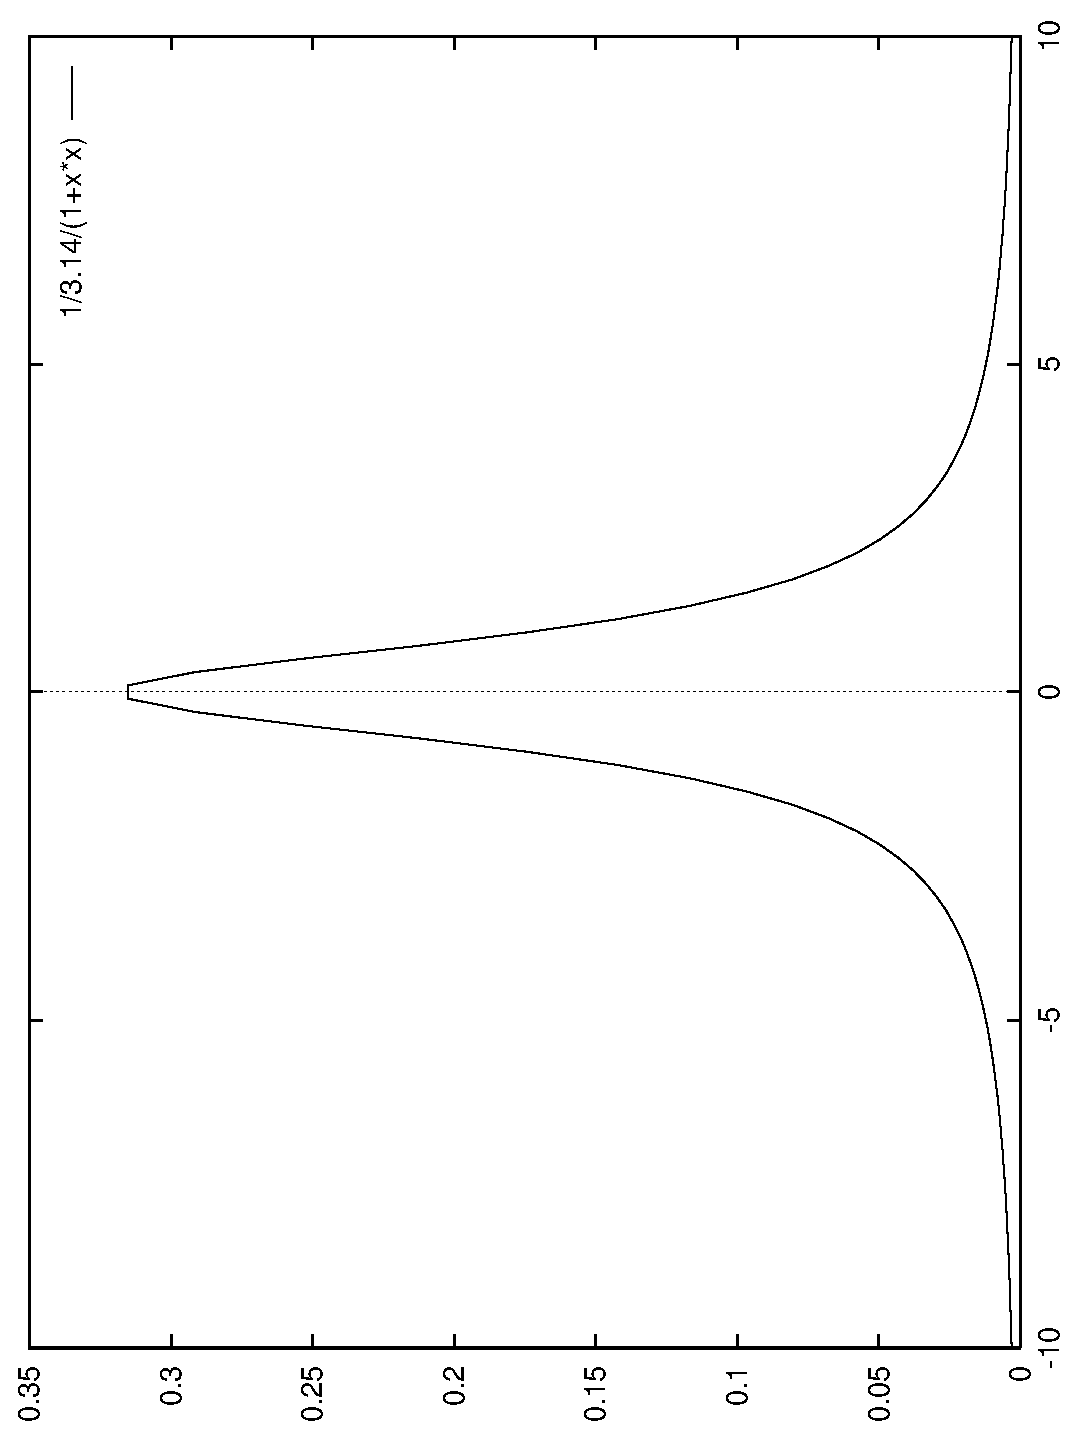
\includegraphics[height=12cm]{cauchy.eps}}\\
\caption{The Cauchy distribution.}
\label{Cauchy}
\end{figure}
\end{center}

\clearpage

\section{Public Methods}

\noindent
These methods can be used by all \cpp - programs, that have included the
header file Cauchy.h and the library EA.

\subsection{Constructors}

%---------------------------------------------------------------------------%
% 001
\index{Cauchy!( )} 
\setNormalInstance
\printEmptyMethodReturn
{}
{Cauchy}
{The default constructor. Generates the random generator of Cauchy distribution.}
{None.}
%---------------------------------------------------------------------------%

%---------------------------------------------------------------------------%
% 002
\index{Cauchy!( RNG\& rng )}
\setNormalInstance
\printMethodWithOneParam
{}
{Cauchy}
{RNG\&}
{rng}
{RNG class.}
{The constructor. Generates the random generator of Cauchy distribution.}
{None.}
{None.}
%---------------------------------------------------------------------------%

\vspace*{10mm}

\subsection{Operators}

%---------------------------------------------------------------------------%
% 003
\index{operator( )!( )} 
\setNormalInstance
\printEmptyMethodReturnSpecial
{double}
{operator( )}
{Gets the result of Cauchy distribution.}
{The factor which was occured by Cauchy distribution.}
{None.}
%---------------------------------------------------------------------------%

\clearpage

\subsection{The probability}

%---------------------------------------------------------------------------%
% 004
\index{p!( const double\& x )} 
\setConstInstance
\printMethodWithOneParam
{double}
{p}
{const double\&}
{x}
{The factor which you want to calculate the probability.}
{Returns the probability of {\em x}.}
{The probability.}
{None.}
%---------------------------------------------------------------------------%









%************************************************************************
% Class DiffGeometric
%************************************************************************
\clearpage
\chapter{Class {\tt DiffGeometric}}
\index{DiffGeometric}
% 24th, Jan, 2001 Ver.1     Tatsuya Okabe
%                 Ver.2
%                 Ver.3
%                 Ver.4
%                 Ver.5
%
%---------------------------------------------------------------------------%
% Made by Tatsuya Okabe ( HONDA R&D Europe ( Deutschland ) GmbH )           %
% Checked by Bernhard Sendhoff ( HONDA R&D Europe ( Deutschland ) GmbH )    %
%---------------------------------------------------------------------------%
% Class DiffGeometric

\section{Abstract}

\noindent
With the class {\em DiffGeometric}, the ``Differentiative Geometiric
distribution'' can be simulated. To calculate this distribution, class
{\em Geometiric} is used twice. After getting two variables from {\em
Geometric}, the random number of {\em DiffGeometirc} is
calculated. This distribution is given by the following equation.

\vspace*{10mm}

\begin{equation}
f(x) = \frac{p \times (1-p)^x}{2-p}
\end{equation}

\vspace*{10mm}

\begin{center}
\begin{figure}[h]
\rotatebox{-90}{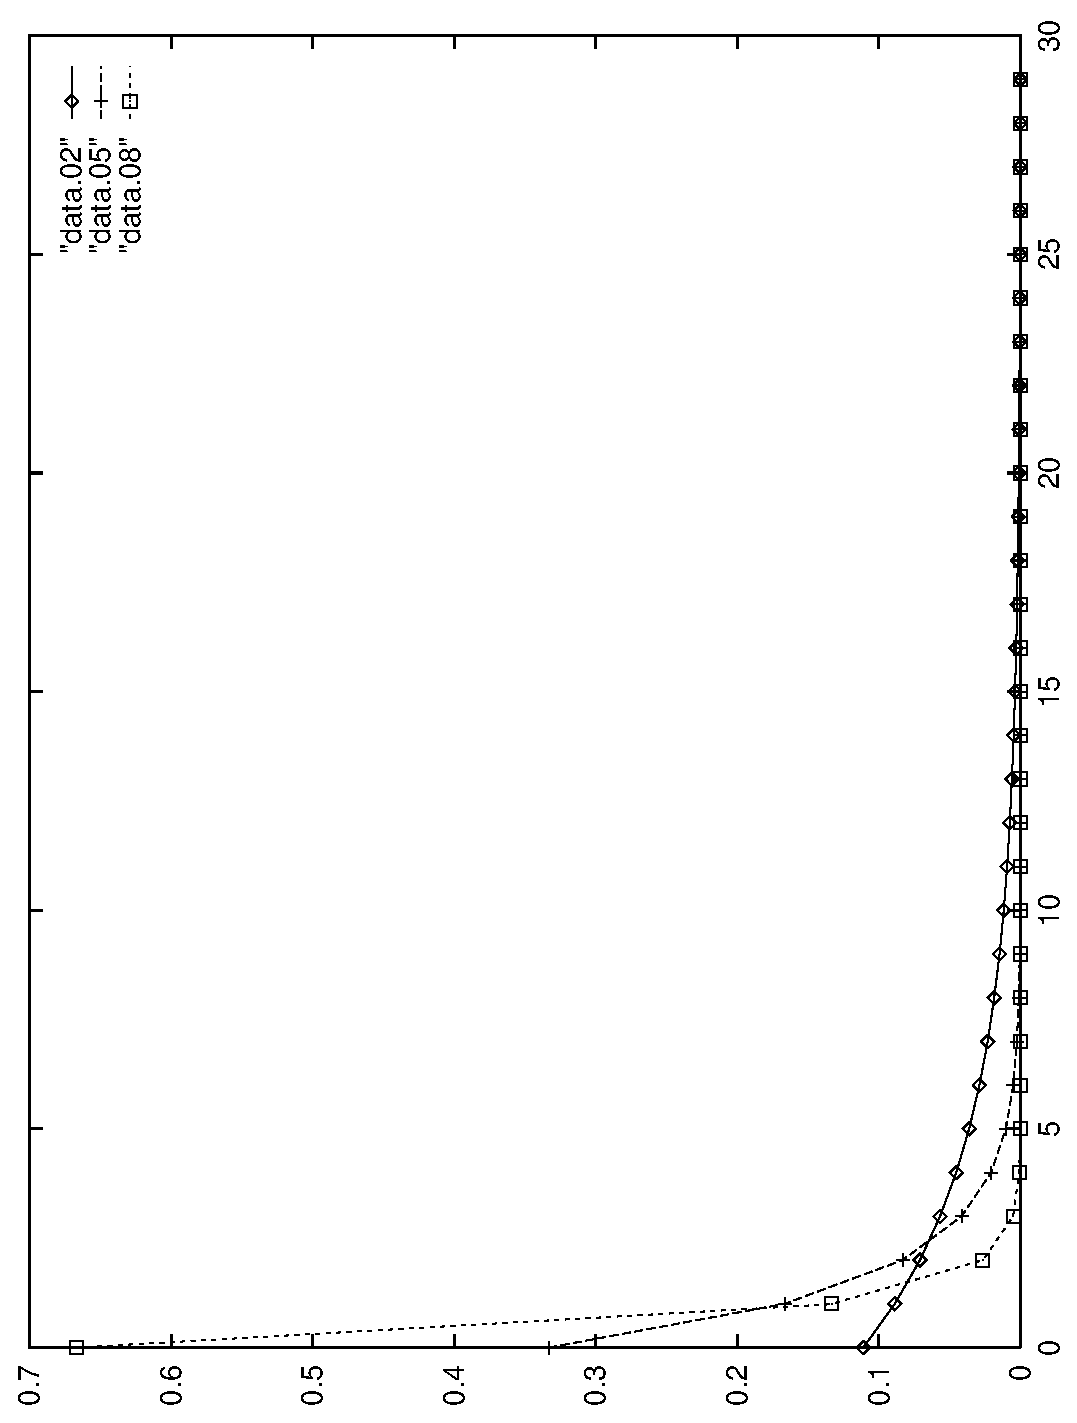
\includegraphics[height=12cm]{diffGeometric.eps}}\\
\caption{The DiffGeometiric distribution with $p = 0.8$ , $0.5$
and $0.2$.}
\end{figure}
\end{center}

\clearpage

\section{Public Methods}

\noindent
These methods can be used by all \cpp - programs, that have included the
header file DiffGeometric.h and the library EA.

\subsection{Constructors}

%---------------------------------------------------------------------------%
% 001
\index{DiffGeometric!( double mean )} 
\setNormalInstance
\printMethodWithOneParam
{}
{DiffGeometric}
{double}
{mean}
{The probability.}
{The default constructor. Generates the random generator of
Differential Geometric distribution.}
{None.}
{None.}
%---------------------------------------------------------------------------%

%---------------------------------------------------------------------------%
% 002
\index{DiffGeometric!( double mean, RNG\& r )}
\setNormalInstance
\setCorrectWidthThree{8pt}
\setParamOne{mean}{double}{The probability.} 
\setParamTwo{r}{RNG\&}{RNG class.}
\printMethodWithParamsSaved
{}
{None.}
{DiffGeometric}
{The constructor. Generates the random generator of Differential
Geometric distribution.}
{None.}
\setCorrectWidthThree{4pt}
%---------------------------------------------------------------------------%

\vspace*{10mm}

\subsection{Operators}

%---------------------------------------------------------------------------%
% 003
\index{operator( )!( double mean )} 
\setNormalInstance
\printMethodWithOneParam
{long}
{operator( )}
{double}
{mean}
{The probability.}
{Gets the result of Differential Geometric distribution.}
{The result of Differential Geometric distribution.}
{None.}
%---------------------------------------------------------------------------%

\clearpage

%---------------------------------------------------------------------------%
% 004
\index{operator( )!( )} 
\setNormalInstance
\printEmptyMethodReturnSpecial
{long}
{operator( )}
{Gets the result of Differential Geometric distribution.}
{The result of Differential Geometric distribution.}
{None.}
%---------------------------------------------------------------------------%

\vspace*{10mm}

\subsection{The probability}

%---------------------------------------------------------------------------%
% 007
\index{p!( const long\& x )} 
\setConstInstance
\printMethodWithOneParam
{double}
{p}
{const long\&}
{x}
{The factor which you want to calculate the probability.}
{Returns the probability of {\em x}.}
{The probability.}
{None.}
%---------------------------------------------------------------------------%





%************************************************************************
% Class DiscreteUniform
%************************************************************************
\clearpage
\chapter{Class {\tt DiscreteUniform}}
\index{DiscreteUniform}
% 24th, Jan, 2001 Ver.1     Tatsuya Okabe
%                 Ver.2
%                 Ver.3
%                 Ver.4
%                 Ver.5
%
%---------------------------------------------------------------------------%
% Made by Tatsuya Okabe ( HONDA R&D Europe ( Deutschland ) GmbH )           %
% Checked by Bernhard Sendhoff ( HONDA R&D Europe ( Deutschland ) GmbH )    %
%---------------------------------------------------------------------------%
% Class DiscreteUniform

\section{Abstract}

\noindent
If we have a set of integers with equal probabilities, the underlying
distribution is called the {\em Discrete Uniform} distribution.

\vspace*{10mm}

\section{Internal variables}

\begin{itemize}
\item {pLow - The lower boundary.}
\item {pHigh - The upper boundary.}
\end{itemize}

%********************
\index{pLow (Variable)}
\index{pHigh (Variable)}
%********************

\vspace*{10mm}

\section{Public Methods}

\noindent
These methods can be used by all \cpp - programs, that have included the
header file DiscreteUniform.h and the library EA.

\subsection{Constructors}

%---------------------------------------------------------------------------%
% 001
\index{DiscreteUniform!( long lo, long hi )}
\setNormalInstance
\setCorrectWidthThree{8pt}
\setParamOne{lo}{long}{The lower boundary.} 
\setParamTwo{hi}{long}{The upper boundary.}
\printMethodWithParamsSaved
{}
{None.}
{DiscreteUniform}
{The default constructor. Generates the random generator of Discrete
Uniform distribution.}
{None.}
\setCorrectWidthThree{4pt}
%---------------------------------------------------------------------------%

\clearpage

%---------------------------------------------------------------------------%
% 002
\index{DiscreteUniform!( long lo, long hi, RNG\& rng )}
\setNormalInstance
\setCorrectWidthThree{8pt}
\setParamOne{lo}{long}{The lower boundary.} 
\setParamTwo{hi}{long}{The upper boundary.}
\setParamThree{rng}{RNG\&}{RNG class.}
\printMethodWithParamsSaved
{}
{None.}
{DiscreteUniform}
{The constructor. Generates the random generator of Discrete Uniform distribution.}
{None.}
\setCorrectWidthThree{4pt}
%---------------------------------------------------------------------------%

\vspace*{10mm}

\subsection{Operators}

%---------------------------------------------------------------------------%
% 003
\index{operator( )!( long lo, long hi )}
\setNormalInstance
\setCorrectWidthThree{8pt}
\setParamOne{lo}{long}{The lower boundary.} 
\setParamTwo{hi}{long}{The upper boundary.}
\printMethodWithParamsSaved
{long}
{The factor which was occured by Discrete Uniform distribution.}
{operator( )}
{Gets the result of Discrete Uniform distribution between {\em lo} and
{\em hi}.}
{None.}
\setCorrectWidthThree{4pt}
%---------------------------------------------------------------------------%

%---------------------------------------------------------------------------%
% 004
\index{operator( )!( )} 
\setNormalInstance
\printEmptyMethodReturnSpecial
{long}
{operator( )}
{Gets the result of Discrete Uniform distribution between {\em pLow}
and {\em pHigh}.}
{The factor which was occured by Discrete Uniform distribution.}
{None.}
%---------------------------------------------------------------------------%

\clearpage

\subsection{Information Retrieval Methods}

%---------------------------------------------------------------------------%
% 005
\index{low!( )} 
\setConstInstance
\printEmptyMethodReturnSpecial
{long}
{low}
{Returns the lower boundary {\em pLow}.}
{The value of the lower boundary {\em pLow}.}
{None.}
%---------------------------------------------------------------------------%

%---------------------------------------------------------------------------%
% 006
\index{high!( )} 
\setConstInstance
\printEmptyMethodReturnSpecial
{long}
{high}
{Returns the upper boundary {\em pHigh}.}
{The value of the upper boundary {\em pHight}.}
{None.}
%---------------------------------------------------------------------------%

%---------------------------------------------------------------------------%
% 007
\index{low!( long lo )} 
\setNormalInstance
\printMethodWithOneParam
{void}
{low}
{long}
{lo}
{New lower boundary.}
{Sets the lower boundary {\em pLow} using new lower boundary.}
{None.}
{None.}
%---------------------------------------------------------------------------%

%---------------------------------------------------------------------------%
% 008
\index{high!( long hi )} 
\setNormalInstance
\printMethodWithOneParam
{void}
{high}
{long}
{hi}
{New upper boundary.}
{Sets the upper boundary {\em pHigh} using new upper boundary.}
{None.}
{None.}
%---------------------------------------------------------------------------%

\clearpage

\subsection{The probability}

%---------------------------------------------------------------------------%
% 009
\index{p!( const long\& x )} 
\setConstInstance
\printMethodWithOneParam
{double}
{p}
{const long\&}
{x}
{The factor which you want to calculate the probability.}
{Returns the probability of {\em x}.}
{The probability.}
{None.}
%---------------------------------------------------------------------------%






%************************************************************************
% Class Erlang
%************************************************************************
%\clearpage
%\chapter{Class {\tt Erlang}}
%\index{Erlang}
%\input{re-Erlang}


%************************************************************************
% Class Geometric
%************************************************************************
\clearpage
\chapter{Class {\tt Geometric}}
\index{Geometric}
% 24th, Jan, 2001 Ver.1     Tatsuya Okabe
%                 Ver.2
%                 Ver.3
%                 Ver.4
%                 Ver.5
%
%---------------------------------------------------------------------------%
% Made by Tatsuya Okabe ( HONDA R&D Europe ( Deutschland ) GmbH )           %
% Checked by Bernhard Sendhoff ( HONDA R&D Europe ( Deutschland ) GmbH )    %
%---------------------------------------------------------------------------%
% Class Geometric

\section{Abstract}

\noindent
With the class {\em Geometric}, we can simulate the ``Geometirc
distribution''. In this distribution, we consider the number of trials
when the factor with the probability {\em p} occurs. The corresponding
equation is as follows.

\begin{equation}
f(x) = p \times ( 1 - p )^{x-1}
\end{equation}

\vspace*{10mm}

\begin{center}
\begin{figure}[h]
\rotatebox{-90}{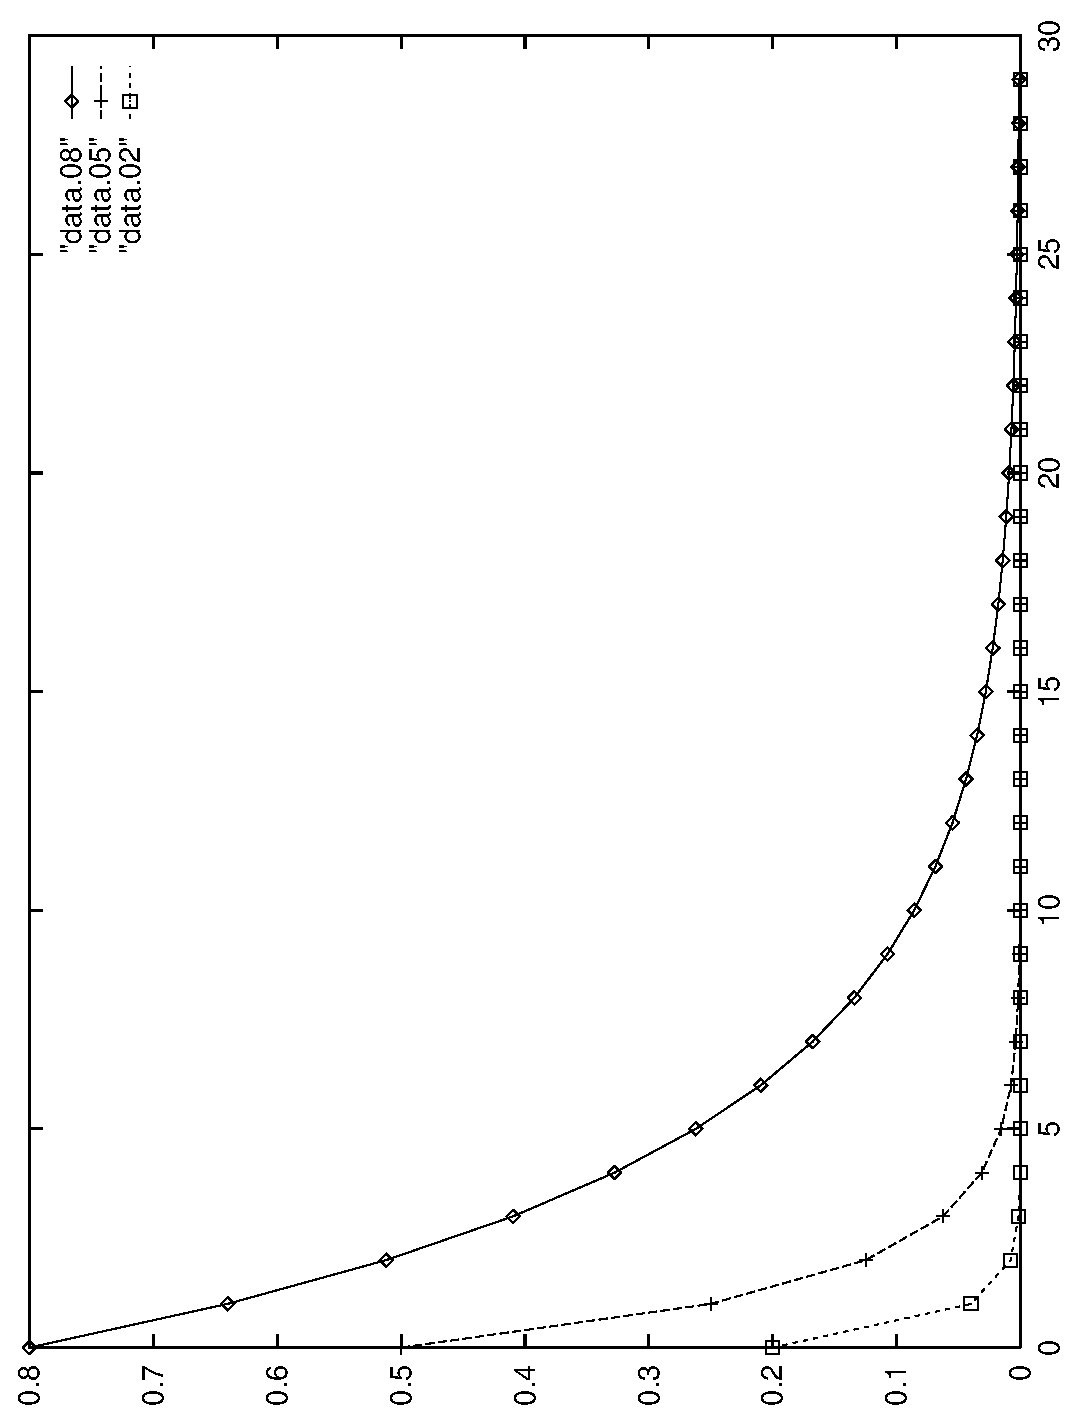
\includegraphics[height=12cm]{geometric.eps}}\\
\caption{The Geometiric distribution $p = 0.8$ , $0.5$ and $0.2$.}
\end{figure}
\end{center}

\clearpage

\section{Internal variables}

\begin{itemize}
\item {pMean - The probability.}
\end{itemize}

%********************
\index{pMean (Variable)}
%********************

\vspace*{10mm}

\section{Public Methods}

\noindent
These methods can be used by all \cpp - programs, that have included the
header file Geometric.h and the library EA.

\subsection{Constructors}

%---------------------------------------------------------------------------%
% 001
\index{Geometric!( double mean )} 
\setNormalInstance
\printMethodWithOneParam
{}
{Geometric}
{double}
{mean}
{The probability.}
{The default constructor. Generates the random generator of Geometric distribution.}
{None.}
{None.}
%---------------------------------------------------------------------------%

%---------------------------------------------------------------------------%
% 002
\index{Geometric!( double mean, RNG\& r )}
\setNormalInstance
\setCorrectWidthThree{8pt}
\setParamOne{mean}{double}{The probability.} 
\setParamTwo{r}{RNG\&}{RNG class.}
\printMethodWithParamsSaved
{}
{None.}
{Geometric}
{The constructor. Generates the random generator of Geometric distribution.}
{None.}
\setCorrectWidthThree{4pt}
%---------------------------------------------------------------------------%

\vspace*{10mm}

\subsection{Operators}

%---------------------------------------------------------------------------%
% 003
\index{operator( )!( double mean )} 
\setNormalInstance
\printMethodWithOneParam
{long}
{operator( )}
{double}
{mean}
{The probability.}
{Gets the number of trials when the factor with the probability {\em mean}
occured firstly.}
{The number of trials.}
{None.}
%---------------------------------------------------------------------------%

\clearpage

%---------------------------------------------------------------------------%
% 004
\index{operator( )!( )} 
\setNormalInstance
\printEmptyMethodReturnSpecial
{long}
{operator( )}
{Gets the number of trials when the factor with the probability {\em pMean}
occured firstly.}
{The number of trials.}
{None.}
%---------------------------------------------------------------------------%

\vspace*{10mm}

\subsection{Information Retrieval Methods}

%---------------------------------------------------------------------------%
% 005
\index{mean!( )} 
\setConstInstance
\printEmptyMethodReturnSpecial
{double}
{mean}
{Returns the probability {\em pMean}.}
{The value of the probability {\em pMean}.}
{None.}
%---------------------------------------------------------------------------%

%---------------------------------------------------------------------------%
% 006
\index{mean!( double newMean )} 
\setNormalInstance
\printMethodWithOneParam
{void}
{mean}
{double}
{newMean}
{New probability.}
{Sets the probability {\em pMean} using new probability {\em newMean}.}
{None.}
{None.}
%---------------------------------------------------------------------------%

\vspace*{10mm}

\subsection{The probability}

%---------------------------------------------------------------------------%
% 007
\index{p!( const long\& x )} 
\setConstInstance
\printMethodWithOneParam
{double}
{p}
{const long\&}
{x}
{The factor which you want to calculate the probability.}
{Returns the probability of {\em x}.}
{The probability.}
{None.}
%---------------------------------------------------------------------------%





%************************************************************************
% Class Rng
%************************************************************************
\clearpage
\chapter{Class {\tt Rng}}
\index{Rng}
% 24th, Jan, 2001 Ver.1     Tatsuya Okabe
%                 Ver.2
%                 Ver.3
%                 Ver.4
%                 Ver.5
%
%---------------------------------------------------------------------------%
% Made by Tatsuya Okabe ( HONDA R&D Europe ( Deutschland ) GmbH )           %
% Checked by Bernhard Sendhoff ( HONDA R&D Europe ( Deutschland ) GmbH )    %
%---------------------------------------------------------------------------%
% Class Rng

\section{Abstract}

\noindent
In this class {\em Rng}, some classes are instantiated. Additionally,
the random seed can be set in the class {\em Rng}.

\vspace*{10mm}

\section{Instantialized classes}

\noindent
Instantialized classes are as follows.

\vspace*{3mm}

\begin{tabular}{lll}
Bernoulli       & $\Longrightarrow$ & Rng::coinToss   \\
DiscreteUniform & $\Longrightarrow$ & Rng::discrete   \\
Uniform         & $\Longrightarrow$ & Rng::uni        \\
Normal          & $\Longrightarrow$ & Rng::gauss      \\
Cauchy          & $\Longrightarrow$ & Rng::cauchy     \\
Geometric       & $\Longrightarrow$ & Rng::geom       \\
DiffGeometric   & $\Longrightarrow$ & Rng::diffGeom   \\
Poisson         & $\Longrightarrow$ & Rng::poisson    \\
\end{tabular}

%********************
\index{Bernoulli}
\index{DiscreteUniform}
\index{Uniform}
\index{Normal}
\index{Cauchy}
\index{Geometric}
\index{DiffGeometric}
\index{Poisson}
\index{Rng::coinToss}
\index{Rng::discrete}
\index{Rng::uni}
\index{Rng::gauss}
\index{Rng::cauchy}
\index{Rng::geom}
\index{Rng::diffGeom}
\index{Rng::poisson}
%********************

\vspace*{3mm}

\section{Public Methods}

\noindent
This method can be used by all \cpp - programs, that have included the
header file GlobalRng.h and the library EA.

\subsection{Initialization Methods}

%---------------------------------------------------------------------------%
% 001
\index{Rng::seed!( long s )}
\setNormalInstance
\printMethodWithOneParam
{void}
{Rng::seed}
{long}
{s}
{Random seed.}
{Initializes a random seed.}
{None.}
{None.}
%---------------------------------------------------------------------------%




%************************************************************************
% Class HyperGeometric
%************************************************************************
%\clearpage
%\chapter{Class {\tt HyperGeometric}}
%\index{HyperGeometric}
%\input{re-HyperGeometric}


%************************************************************************
% Class LogNormal
%************************************************************************
\clearpage
\chapter{Class {\tt LogNormal}}
\index{LogNormal}
% 24th, Jan, 2001 Ver.1     Tatsuya Okabe
%                 Ver.2
%                 Ver.3
%                 Ver.4
%                 Ver.5
%
%---------------------------------------------------------------------------%
% Made by Tatsuya Okabe ( HONDA R&D Europe ( Deutschland ) GmbH )           %
% Checked by Bernhard Sendhoff ( HONDA R&D Europe ( Deutschland ) GmbH )    %
%---------------------------------------------------------------------------%
% Class LogNormal

\section{Abstract}

\noindent
With the class {\em LogNormal}, we can simulate the ``Log Normal''
distribution. If the logarithm $log(x)$ is normally or {\em Gaussian}
distributed, the distribution of {\em x} is called the {\em Log
Normal} distribution. The equation for this distribution is given below.

\begin{equation}
f(x) = \left\{
\begin{array}{ll}
\frac{1}{\sqrt{2\pi} \sigma x} \cdot \exp \left\{ \frac{-(\log x - \mu )^2}{2 \sigma^2} \right\} & x>0 \\
0 & x \le 0
\end{array}
\right.
\end{equation}

\noindent
In this equation, $x$, $\sigma$ and $\mu$ mean the variable, the
deviation and the average, respectively.

\vspace*{10mm}

\begin{center}
\begin{figure}[h]
\rotatebox{-90}{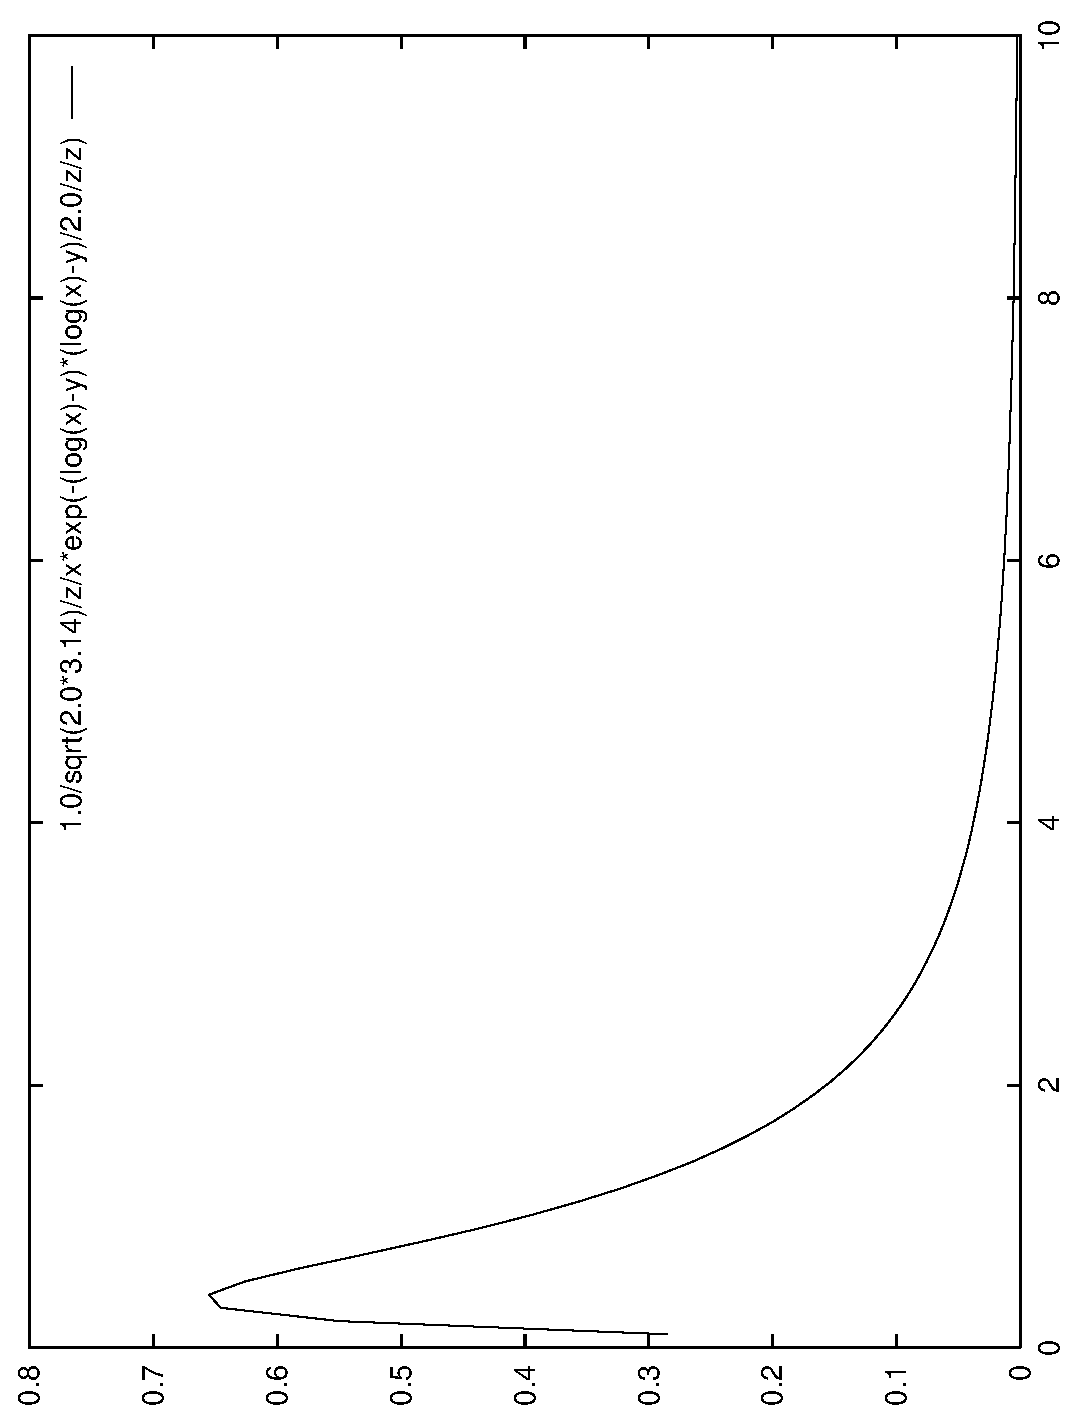
\includegraphics[height=12cm]{lognormal.eps}}\\
\caption{The Log Normal distribution. $\sigma=e(e-1)$ , $\mu=\sqrt{e}$.}
\end{figure}
\end{center}

\clearpage

\section{Internal Variables}

\begin{itemize}
\item logMean - The average.
\item logVariance - The variance.
\end{itemize}

%********************
\index{logMean (Variable)}
\index{logVariance (Variable)}
%********************

\vspace*{10mm}

\section{Public Methods}

\noindent
These methods can be used by all \cpp - programs, that have included the
header file LogNormal.h and the library EA. If you declare only
Population.h, we can't use these methods in this version.

\subsection{Constructors}

%---------------------------------------------------------------------------%
% 001
\index{LogNormal!( double mean, double variance )}
\setNormalInstance
\setCorrectWidthThree{8pt}
\setParamOne{mean}{double}{The average.} 
\setParamTwo{variance}{double}{The variance.}
\printMethodWithParamsSaved
{}
{None.}
{LogNormal}
{The default constructor. Generates the random generator of Log Normal
distribution.}
{None.}
\setCorrectWidthThree{4pt}
%---------------------------------------------------------------------------%

%---------------------------------------------------------------------------%
% 002
\index{LogNormal!( double mean, double variance, RNG\& rng )}
\setNormalInstance
\setCorrectWidthThree{8pt}
\setParamOne{mean}{double}{The average.} 
\setParamTwo{variance}{double}{The variance.}
\setParamThree{rng}{RNG\&}{RNG class.}
\printMethodWithParamsSaved
{}
{None..}
{LogNormal}
{The constructor. Generates the random generator of Log Normal distribution.}
{None.}
\setCorrectWidthThree{4pt}
%---------------------------------------------------------------------------%

\clearpage

\subsection{Operators}

%---------------------------------------------------------------------------%
% 003
\index{operator( )!( )} 
\setNormalInstance
\printEmptyMethodReturnSpecial
{double}
{operator( )}
{Gets the result of the log normal distribution.}
{The result of the log normal distribution.}
{None.}
%---------------------------------------------------------------------------%

%---------------------------------------------------------------------------%
% 004
\index{operator( )!( double mean, double variance )}
\setNormalInstance
\setCorrectWidthThree{8pt}
\setParamOne{mean}{double}{The average.} 
\setParamTwo{variance}{double}{The variance.}
\printMethodWithParamsSaved
{}
{The result of the log normal distribution.}
{operator( )}
{Gets the result of the log normal distribution.}
{None.}
\setCorrectWidthThree{4pt}
%---------------------------------------------------------------------------%

\vspace*{10mm}

\subsection{Information Retrieval Methods}

%---------------------------------------------------------------------------%
% 005
\index{mean!( )} 
\setConstInstance
\printEmptyMethodReturnSpecial
{double}
{mean}
{Returns the mean {\em logMean}.}
{The mean {\em logMean}.}
{None.}
%---------------------------------------------------------------------------%

%---------------------------------------------------------------------------%
% 006
\index{variance!( )} 
\setConstInstance
\printEmptyMethodReturnSpecial
{double}
{variance}
{Returns the variance {\em logVariance}.}
{The variance {\em logVariance}.}
{None.}
%---------------------------------------------------------------------------%

\clearpage

%---------------------------------------------------------------------------%
% 007
\index{mean!(double newMean )} 
\setNormalInstance
\printMethodWithOneParam
{void}
{mean}
{double}
{newMean}
{New mean.}
{Sets the mean {\em logMean} using {\em newMean} and also sets the variables
{\em pMean} and {\em pStdDev}.}
{None.}
{None.}
%---------------------------------------------------------------------------%

%---------------------------------------------------------------------------%
% 008
\index{variance!(double newVariance )} 
\setNormalInstance
\printMethodWithOneParam
{void}
{variance}
{double}
{newVar}
{New variance.}
{Sets the variance {\em logVariance} using {\em newVariance} and also
sets the variables {\em pMean} and {\em pStdDev}.}
{None.}
{None.}
%---------------------------------------------------------------------------%

\vspace*{10mm}

\subsection{The probability}

%---------------------------------------------------------------------------%
% 009
\index{p!( const double\& x )} 
\setConstInstance
\printMethodWithOneParam
{double}
{p}
{const double\&}
{x}
{The factor which you want to calculate the probability.}
{Returns the probability of {\em x}.}
{The probability.}
{None.}
%---------------------------------------------------------------------------%

\clearpage

\section{Private Methods}

%---------------------------------------------------------------------------%
% 010
\index{setState!( )} 
\setNormalInstance
\printEmptyMethod
{setState}
{Calculates the variables {\em pMean} and {\em pStdDev} from {\em
logMean} and {\em logVariance}.}
%---------------------------------------------------------------------------%

\noindent
The relationships among these variables are as follows.

\begin{equation}
\mu_N = \log{\left( \frac{\mu_L^2}{\sqrt{\mu_L^2 + \sigma_L^2}}
\right)}
\end{equation}

\begin{equation}
\sigma_N = \sqrt{ \log{\left( \frac{\mu_L^2 + \sigma_L^2}{\mu_L^2}
\right)} }
\end{equation}

\noindent
Here, $\mu_N$, $\sigma_N$, $\mu_L$ and $\sigma_L$ are {\em pMean},
{\em pStdDev}, {\em logMean} and the square root of {\em logVariance} respectively.


%************************************************************************
% Class NegExponential
%************************************************************************
\clearpage
\chapter{Class {\tt NegExponential}}
\index{NegExponential}
% 24th, Jan, 2001 Ver.1     Tatsuya Okabe
%                 Ver.2
%                 Ver.3
%                 Ver.4
%                 Ver.5
%
%---------------------------------------------------------------------------%
% Made by Tatsuya Okabe ( HONDA R&D Europe ( Deutschland ) GmbH )           %
% Checked by Bernhard Sendhoff ( HONDA R&D Europe ( Deutschland ) GmbH )    %
%---------------------------------------------------------------------------%
% Class NegExponential

\section{Abstract}

\noindent
With the class {\em NegExponential}, we can calculate the ``Negative
Exponential'' distribution with the following equation.

\begin{equation}
f(x) = \frac{1}{a} \cdot \exp\left\{\frac{-x^2}{a}\right\}
\end{equation}

\noindent
In this equation, $a$ and $x$ mean the constant value and the variable respectively.

\vspace*{10mm}

\begin{center}
\begin{figure}[h]
\rotatebox{-90}{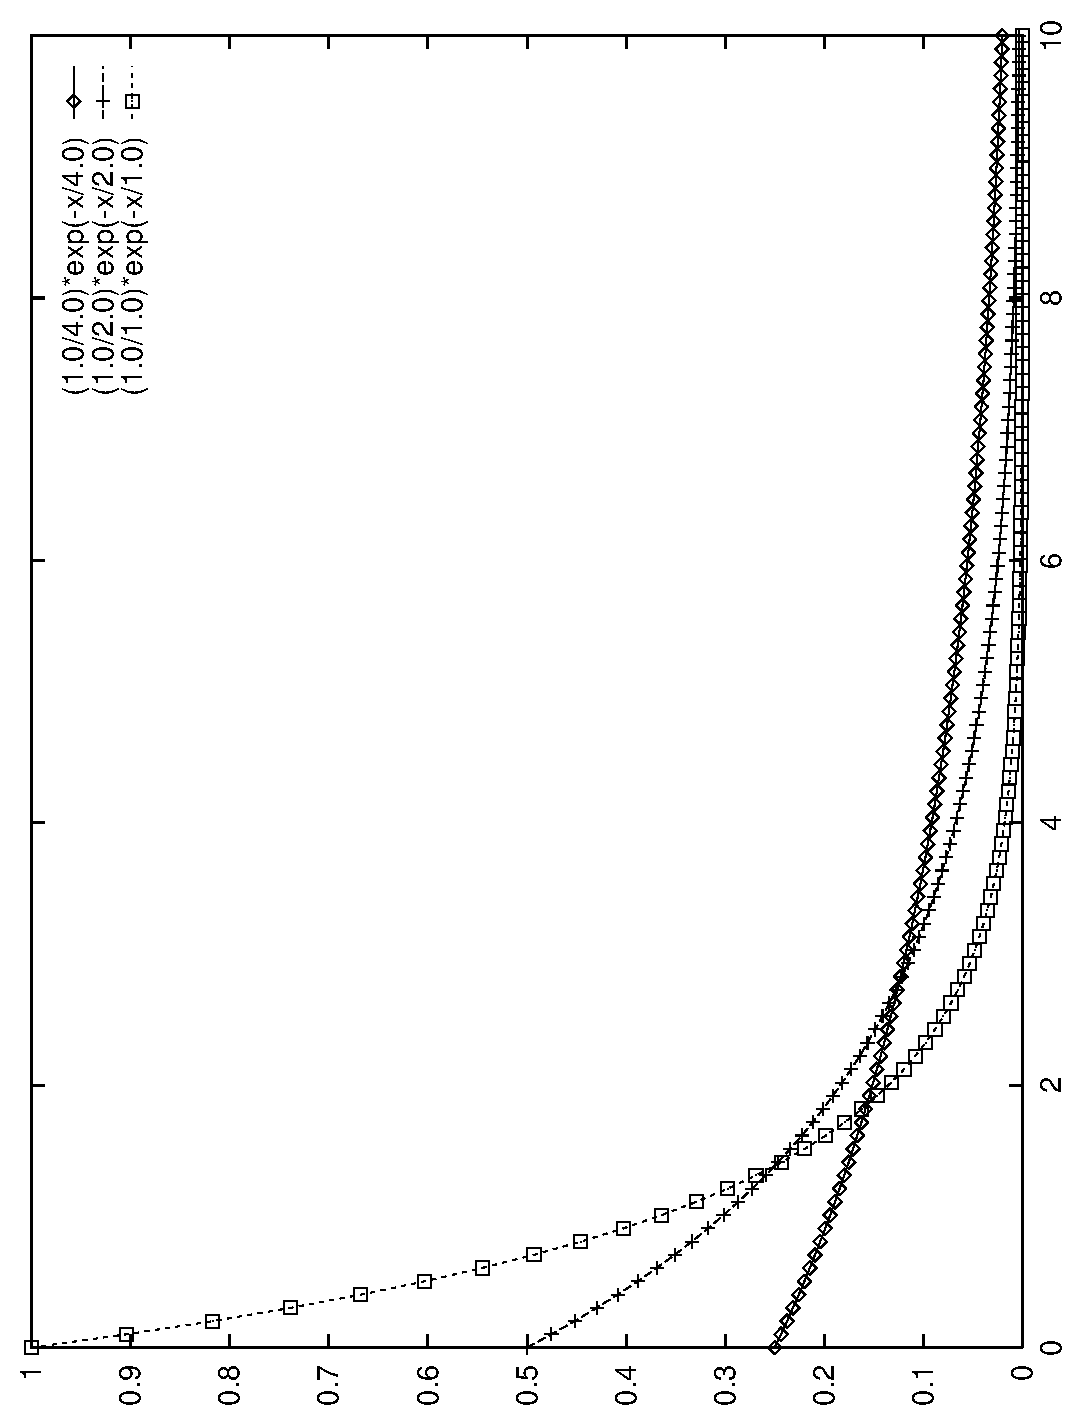
\includegraphics[height=12cm]{negexponential.eps}}\\
\caption{The Negative exponential distribution $a=1,2,4$.}
\end{figure}
\end{center}

\clearpage

\section{Internal Variables}

\begin{itemize}
\item pMean - The constant variable $a$ in the former equation.
\end{itemize}

%********************
\index{pMean (Variable)}
%********************

\vspace*{5mm}

\section{Public Methods}

\noindent
These methods can be used by all \cpp - programs, that have included the
header file NegExponential.h and the library EA. If you declare only
Population.h, we can't use these methods in this version.

\subsection{Constructors}

%---------------------------------------------------------------------------%
% 001
\index{NegExponential!( double mean )}
\setNormalInstance
\printMethodWithOneParam
{}
{NegExponential}
{double}
{mean}
{The constant variable $a$.}
{The default constructor. Generates the random generator of Negative
Exponential distribution.}
{None.}
{None.}
%---------------------------------------------------------------------------%

%---------------------------------------------------------------------------%
% 002
\index{NegExponential!( double mean, RNG\& r )}
\setNormalInstance
\setCorrectWidthThree{8pt}
\setParamOne{mean}{double}{The constant variable $a$.} 
\setParamTwo{r}{RNG\&}{RNG class}
\printMethodWithParamsSaved
{}
{None.}
{NegExponential}
{The constructor. Generates the random generator of Negative
Exponential distribution.}
{None.}
\setCorrectWidthThree{4pt}
%---------------------------------------------------------------------------%

\vspace*{5mm}

\subsection{Operators}

%---------------------------------------------------------------------------%
% 003
\index{operator( )!( double mean )} 
\setNormalInstance
\printMethodWithOneParam
{double}
{operator( )}
{double}
{mean}
{The constant variable $a$.}
{Gets the result of Negative Exponential distribution.}
{The result of Negative Exponential distribution.}
{None.}
%---------------------------------------------------------------------------%

\clearpage

%---------------------------------------------------------------------------%
% 004
\index{operator( )!( )} 
\setNormalInstance
\printEmptyMethodReturnSpecial
{double}
{operator( )}
{Gets the result of Negative Exponential  distribution.}
{The result of Negative Exponential distribution.}
{None.}
%---------------------------------------------------------------------------%

\vspace*{10mm}

\subsection{Information Retrieval Methods}

%---------------------------------------------------------------------------%
% 005
\index{mean!( )} 
\setConstInstance
\printEmptyMethodReturnSpecial
{double}
{mean}
{Returns the varible {\em pMean}.}
{The variable {\em pMean}.}
{None.}
%---------------------------------------------------------------------------%

%---------------------------------------------------------------------------%
% 006
\index{mean!( double newMean )} 
\setNormalInstance
\printMethodWithOneParam
{void}
{mean}
{double}
{newMean}
{New constant variable {\em pMean}.}
{Sets the constant variable {\em pMean} using new variable {\em newMean}.}
{None.}
{None.}
%---------------------------------------------------------------------------%

\vspace*{10mm}

\subsection{The probability}

%---------------------------------------------------------------------------%
% 007
\index{p!( const double\& x )} 
\setConstInstance
\printMethodWithOneParam
{double}
{p}
{const double\&}
{x}
{The factor which you want to calculate the probability.}
{Returns the probability of {\em x}.}
{The probability.}
{None.}
%---------------------------------------------------------------------------%






%************************************************************************
% Class Normal
%************************************************************************
\clearpage
\chapter{Class {\tt Normal}}
\index{Normal}
% 24th, Jan, 2001 Ver.1     Tatsuya Okabe
%                 Ver.2
%                 Ver.3
%                 Ver.4
%                 Ver.5
%
%---------------------------------------------------------------------------%
% Made by Tatsuya Okabe ( HONDA R&D Europe ( Deutschland ) GmbH )           %
% Checked by Bernhard Sendhoff ( HONDA R&D Europe ( Deutschland ) GmbH )    %
%---------------------------------------------------------------------------%
% Class Normal

\section{Abstract}

\noindent
With the class {\em Normal}, the ``Normal'' or ``Gaussian''
distribution can be simulated. The corresponding equation is given below.

\begin{equation}
f(x) = \frac{1}{\sqrt{2\pi}\sigma} \cdot \exp{\frac{-(x-\mu)^2}{2\sigma^2}}
\end{equation}

\noindent
In this equation, $x$, $\sigma$ and $\mu$ mean the factor, the deviation
and the average, respectively.

\noindent
In this class, Box-Muller method was used to generate the random
numbers. Please refer [\ref{NRC}] to get more information.

%********************
\index{Box-Muller Method}
%********************

\vspace*{10mm}

\begin{center}
\begin{figure}[h]
\rotatebox{-90}{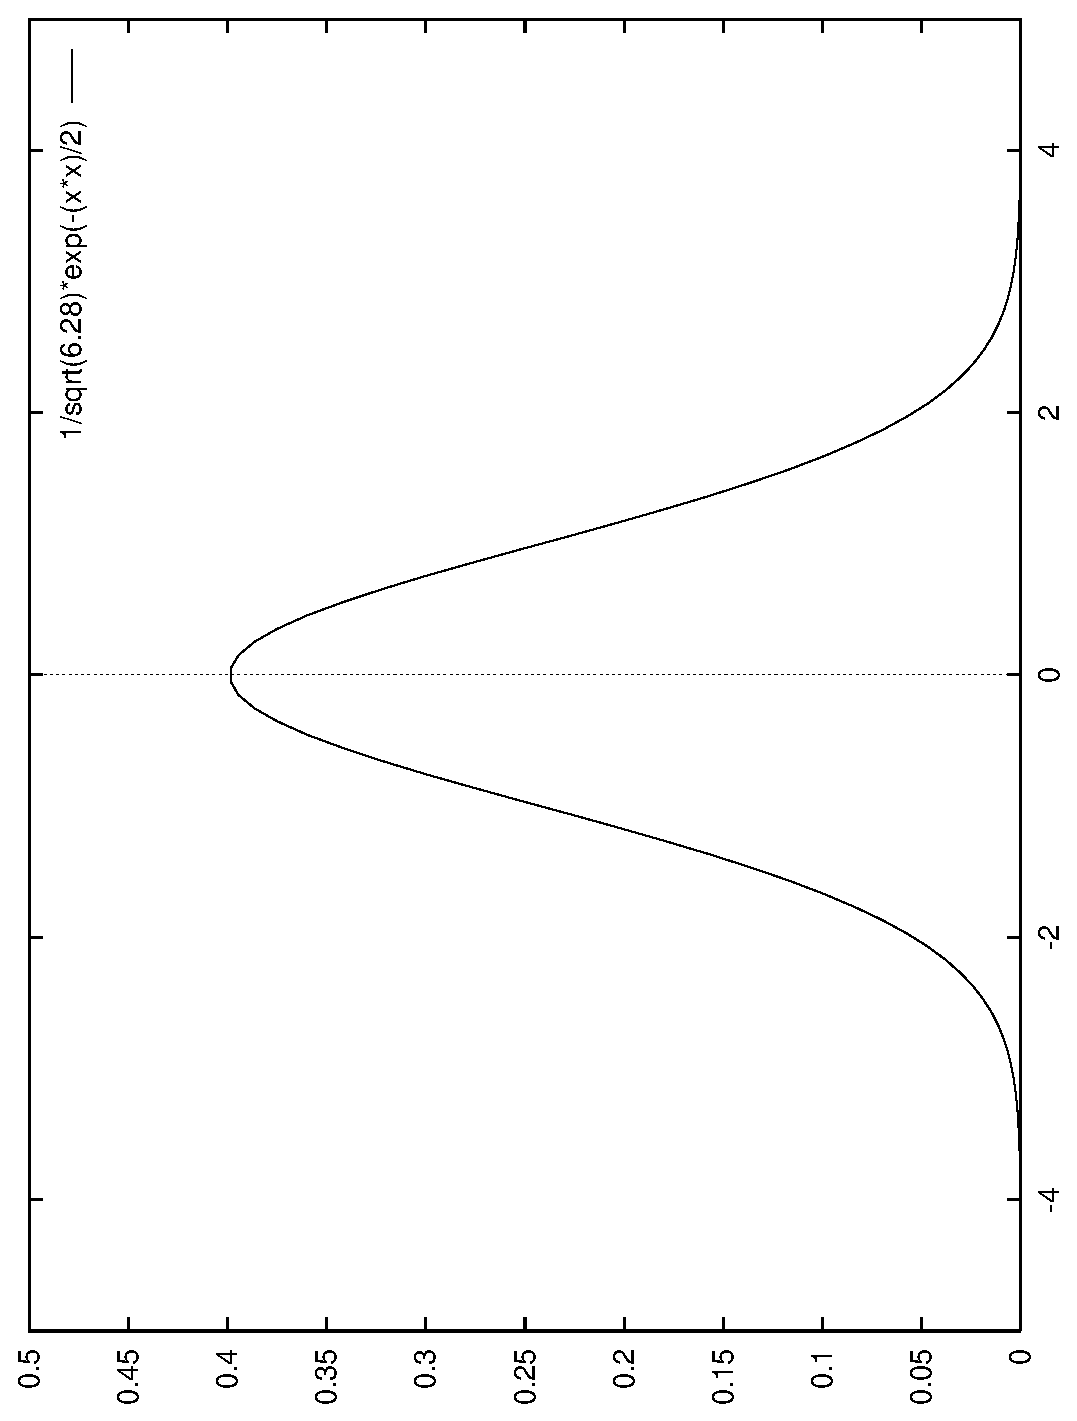
\includegraphics[height=12cm]{normal.eps}}\\
\caption{The Normal distribution. $\sigma=1$ and $\mu=0$.}
\end{figure}
\end{center}

\clearpage

\section{Internal Variables}

\begin{itemize}
\item pMean - The average.
\item pStdDev - The deviation.
\item iset - The flag in Box-Muller method ( existance of random
number ).
\item gset - The variable to store the random number.
\end{itemize}

%********************
\index{pMean (Variable)}
\index{pStdDev (Variable)}
\index{iset (Variable)}
\index{gset (Variable)}
%********************

\vspace*{10mm}

\section{Public Methods}

\noindent
These methods can be used by all \cpp - programs, that have included the
header file Normal.h and the library EA.

\subsection{Constructors}

%---------------------------------------------------------------------------%
% 001
\index{Normal!( double mean, double variance )}
\setNormalInstance
\setCorrectWidthThree{8pt}
\setParamOne{mean}{double}{The average.} 
\setParamTwo{variance}{double}{The variance.}
\printMethodWithParamsSaved
{}
{None.}
{Normal}
{The default constructor. Generates the random generator of Normal distribution.}
{None.}
\setCorrectWidthThree{4pt}
%---------------------------------------------------------------------------%

%---------------------------------------------------------------------------%
% 002
\index{Normal!( double mean, double variance, RNG\& rng )}
\setNormalInstance
\setCorrectWidthThree{8pt}
\setParamOne{mean}{double}{The average.} 
\setParamTwo{variance}{double}{The variance.}
\setParamThree{rng}{RNG\&}{RNG class.}
\printMethodWithParamsSaved
{}
{None.}
{Normal}
{The constructor. Generates the random generator of Normal distribution.}
{None.}
\setCorrectWidthThree{4pt}
%---------------------------------------------------------------------------%

\clearpage

\subsection{Operators}

%---------------------------------------------------------------------------%
% 003
\index{operator( )!( double mean, double variance )}
\setNormalInstance
\setCorrectWidthThree{8pt}
\setParamOne{mean}{double}{The average.} 
\setParamTwo{variance}{double}{The variance.}
\printMethodWithParamsSaved
{double}
{The result of normal distribution {\em N( mean, variance )}.}
{operator}
{Gets the result of normal distribution {\em N( mean, variance )}.}
{None.}
\setCorrectWidthThree{4pt}
%---------------------------------------------------------------------------%

%---------------------------------------------------------------------------%
% 004
\index{operator( )!( )} 
\setNormalInstance
\printEmptyMethodReturnSpecial
{double}
{operator( )}
{Gets the result of normal distribution {\em N( pMean, (pStdDev)$^2$ )}.}
{The result of normal distribution {\em N( pMean, (pStdDev)$^2$ )}.}
{None.}
%---------------------------------------------------------------------------%

\vspace*{10mm}

\subsection{Information Retrieval Methods}

%---------------------------------------------------------------------------%
% 005
\index{mean!( )} 
\setConstInstance
\printEmptyMethodReturnSpecial
{double}
{mean}
{Returns the average {\em pMean}.}
{The average {\em pMean}.}
{None.}
%---------------------------------------------------------------------------%

%---------------------------------------------------------------------------%
% 006
\index{variance!( )} 
\setConstInstance
\printEmptyMethodReturnSpecial
{double}
{variance}
{Returns the variance {\em (pStdDev)$^2$}.}
{The variance {\em (pStdDev)$^2$}.}
{None.}
%---------------------------------------------------------------------------%

\clearpage

%---------------------------------------------------------------------------%
% 007
\index{mean!( double newMean )} 
\setNormalInstance
\printMethodWithOneParam
{void}
{mean}
{double}
{newMean}
{New value of the average.}
{Sets the average {\em pMean} using new average {\em newMean}.}
{None.}
{None.}
%---------------------------------------------------------------------------%

%---------------------------------------------------------------------------%
% 008
\index{variance!( double newVar )} 
\setNormalInstance
\printMethodWithOneParam
{void}
{variance}
{double}
{newVar}
{New value of the variance.}
{Sets the deviation {\em pStdDev} using square root of new variance
{\em newVar}.}
{None.}
{None.}
%---------------------------------------------------------------------------%

\vspace*{10mm}

\subsection{Random seed}

%---------------------------------------------------------------------------%
% 009
\index{seed!( long s )} 
\setNormalInstance
\printMethodWithOneParam
{void}
{seed}
{long}
{s}
{Random seed.}
{Initializes the random seed.}
{None.}
{None.}
%---------------------------------------------------------------------------%

\vspace*{10mm}

\subsection{The probability}

%---------------------------------------------------------------------------%
% 010
\index{p!( const double\& x )} 
\setConstInstance
\printMethodWithOneParam
{double}
{p}
{const double\&}
{x}
{The factor which you want to calculate the probability.}
{Returns the probability of {\em x}.}
{The probability.}
{None.}
%---------------------------------------------------------------------------%
















%************************************************************************
% Class Poisson
%************************************************************************
\clearpage
\chapter{Class {\tt Poisson}}
\index{Poisson}
% 24th, Jan, 2001 Ver.1     Tatsuya Okabe
%                 Ver.2
%                 Ver.3
%                 Ver.4
%                 Ver.5
%
%---------------------------------------------------------------------------%
% Made by Tatsuya Okabe ( HONDA R&D Europe ( Deutschland ) GmbH )           %
% Checked by Bernhard Sendhoff ( HONDA R&D Europe ( Deutschland ) GmbH )    %
%---------------------------------------------------------------------------%
% Class Poisson

\section{Abstract}

\noindent
With the class {\em Poisson}, we can simulate the ``Poisson''
distribution. Now let's guess the situation where we try somethings
$n$ times and we saw the factor $x$ times with the probability
$p$. This distribution follows ``Binomial'' distribution as the next
equation. 

\begin{equation}
f(x) = _n \hspace{-2mm} C_x p^x (1-p)^{n-x} = \frac{n!}{x! (n-x)!} p^x (1-p)^{n-x}
\end{equation} 

\noindent
If the number of experiences is sufficiently large, this equation can
be approximated by ``Poisson'' distribution, which will be shown in
the next equation.

\begin{equation}
f(x) = \frac{e^\lambda \lambda^x}{x!}
\end{equation}

\noindent
In this equation, $\lambda$ and x mean the constant and the factor respectively.

\vspace*{10mm}

\section{Internal Variables}

\begin{itemize}
\item pMean - Corresponding to $\lambda$ in upper equation.
\end{itemize}

%********************
\index{pMean (Variable)}
%********************

\clearpage

\section{Public Methods}

\noindent
These methods can be used by all \cpp - programs, that have included the
header file Poisson.h and the library EA.

\subsection{Constructors}

%---------------------------------------------------------------------------%
% 001
\index{Poisson!( double mean )}
\setNormalInstance
\printMethodWithOneParam
{}
{Poisson}
{double}
{mean}
{The constant $\lambda$.}
{The default constructor. Generates the random generator of Poisson distribution.}
{None.}
{None.}
%---------------------------------------------------------------------------%

%---------------------------------------------------------------------------%
% 002
\index{Poisson!( double mean, RNG\& r )}
\setNormalInstance
\setCorrectWidthThree{8pt}
\setParamOne{mean}{double}{The constant $\lambda$.} 
\setParamTwo{r}{RNG\&}{RNG class.}
\printMethodWithParamsSaved
{}
{None.}
{Poisson}
{The constructor. Generates the random generator of Poisson distribution.}
{None.}
\setCorrectWidthThree{4pt}
%---------------------------------------------------------------------------%

\vspace*{10mm}

\subsection{Operators}

%---------------------------------------------------------------------------%
% 003
\index{operetor( )!( double mean )}
\setNormalInstance
\printMethodWithOneParam
{long}
{operator( )}
{double}
{mean}
{The constant $\lambda$.}
{Gets the result of Poisson distribution.}
{The result of Poisson distribution.}
{None.}
%---------------------------------------------------------------------------%

\clearpage

%---------------------------------------------------------------------------%
% 004
\index{operator( )!( )} 
\setNormalInstance
\printEmptyMethodReturnSpecial
{long}
{operator( )}
{Gets the result of Poisson distribution {\em ( $\lambda$ = pMean )}.}
{The result of Poisson distribution {\em ( $\lambda$ = pMean )}.}
{None.}
%---------------------------------------------------------------------------%

\vspace*{10mm}

\subsection{Information Retrieval Methods}

%---------------------------------------------------------------------------%
% 005
\index{mean!( )} 
\setConstInstance
\printEmptyMethodReturnSpecial
{double}
{mean}
{Returns the variable {\em $\lambda$} {\em pMean}.}
{The variable {\em $\lambda$} {\em pMean}.}
{None.}
%---------------------------------------------------------------------------%

%---------------------------------------------------------------------------%
% 006
\index{mean!( double newMean )} 
\setNormalInstance
\printMethodWithOneParam
{void}
{mean}
{double}
{newMean}
{New $\lambda$.}
{Sets the mean {\em pMean} using new mean {\em newMean}.}
{None.}
{None.}
%---------------------------------------------------------------------------%

\vspace*{10mm}

\subsection{The probability}

%---------------------------------------------------------------------------%
% 007
\index{p!( const long\& x )} 
\setConstInstance
\printMethodWithOneParam
{double}
{p}
{const long\&}
{x}
{The factor which you want to calculate the probability.}
{Returns the probability of {\em x}.}
{The probability.}
{None.}
%---------------------------------------------------------------------------%






%************************************************************************
% Class RNG
%************************************************************************
\clearpage
\chapter{Class {\tt RNG}}
\index{RNG}
% 24th, Jan, 2001 Ver.1     Tatsuya Okabe
%                 Ver.2
%                 Ver.3
%                 Ver.4
%                 Ver.5
%
%---------------------------------------------------------------------------%
% Made by Tatsuya Okabe ( HONDA R&D Europe ( Deutschland ) GmbH )           %
% Checked by Bernhard Sendhoff ( HONDA R&D Europe ( Deutschland ) GmbH )    %
%---------------------------------------------------------------------------%
% Class RNG

\section{Abstract}

\noindent
In the class {\em RNG}, we can set the random seed value. Also, class
{\em RNG} was instantialized as {\em globalRng}.

\noindent
A computer seems to be able to generate random numbers. But, we should
call them ``pseudo random number'' because we can expect. The reason
why we can do this is that C++ or Fortran uses the following equation
to generate a random number.

\begin{equation}
I_{j+1} = a I_{j} + c \hspace{10mm} ( mod \hspace{5mm} m )
\end{equation}

\noindent
Here, $I$, $a$, $c$ and $m$ are random number, multiplier, increment
and modulus, respectively. Specially, $I_0$ is called ``random seed''.

\noindent
This method is called ``linear congruential method''.

\noindent
This equation shows that generated random numbers are cyclic and the
longest frequency is $m$. However, if we failed to select the correct
values of $a$, $c$ and $m$, the frequency will be shortened. Thus,
many mathematicians researched these values.

\noindent
Park and Miller proposed ``Minimal Standard generater'' in 1988. In
the method, they proposed following values.

\begin{equation}
a = 7^5 = 16807 \hspace{10mm} m = 2^{31} - 1 = 2147483647
\hspace{10mm} c = 0
\end{equation}

\noindent
For more information, please see [\ref{NRC}].

\vspace*{10mm}

\section{Instantialized classes}

\noindent
Instantialized classes are as follows.

\vspace*{3mm}

\begin{tabular}{lll}
RNG       & $\Longrightarrow$ & globalRng   \\
\end{tabular}

\vspace*{3mm}

\section{Internal Variables}

\begin{itemize}
\item initialSx - Initial value of random seed 1.
\item initialSy - Initial value of random seed 2.
\item initialSz - Initial value of random seed 3.
\item sx - Current value of random seed 1.
\item sy - Current value of random seed 2.
\item sz - Current value of random seed 3.
\end{itemize}

%********************
\index{initialSx (Variable)}
\index{initialSy (Variable)}
\index{initialSz (Variable)}
\index{sx (Variable)}
\index{sy (Variable)}
\index{sz (Variable)}
%********************

\vspace*{10mm}

\section{Public Methods}

\noindent
This method can be used by all \cpp - programs, that have included the
header file RNG.h and the library EA.

\subsection{Constructors}

%---------------------------------------------------------------------------%
% 001
\index{RNG!( long s )}
\setNormalInstance
\printMethodWithOneParam
{}
{RNG}
{long}
{s}
{Random seed.}
{The default constructor. Gerenates this class.}
{None.}
{None.}
%---------------------------------------------------------------------------%

\vspace*{10mm}

\subsection{Operators}

%---------------------------------------------------------------------------%
% 002
\index{operator( )!( )}
\setNormalInstance
\printEmptyMethodReturnSpecial
{double}
{operator}
{Gets a random seed for double type.}
{A random seed.}
{None.}
%---------------------------------------------------------------------------%

\clearpage

\subsection{Information Retrieval Methods}

%---------------------------------------------------------------------------%
% 003
\index{seed!( long s )}
\setNormalInstance
\printMethodWithOneParam
{void}
{seed}
{long}
{s}
{Random seed.}
{Sets initial variables and current variables regaring a random seed.}
{None.}
{None.}
%---------------------------------------------------------------------------%

%---------------------------------------------------------------------------%
% 004
\index{reset!( )}
\setNormalInstance
\printEmptyMethod
{reset}
{Initializes current variables.}
%---------------------------------------------------------------------------%

%---------------------------------------------------------------------------%
% 005
\index{genLong!( )}
\setNormalInstance
\printEmptyMethodReturnSpecial
{long}
{genLong}
{Gets a random seed for long type.}
{A random seed.}
{None.}
%---------------------------------------------------------------------------%

%---------------------------------------------------------------------------%
% 006
\index{genDouble!( )}
\setNormalInstance
\printEmptyMethodReturnSpecial
{double}
{genDouble}
{Gets a random seed for double type.}
{A random seed.}
{None.}
%---------------------------------------------------------------------------%

\clearpage

%---------------------------------------------------------------------------%
% 007
\index{getStatus!( unsigned $\&$x, unsigned $\&$y, unsigned $\&$z )}
\setConstInstance
\setCorrectWidthThree{8pt}
\setParamOne{$\&$x}{unsigned}{A random seed 1.} 
\setParamTwo{$\&$y}{unsigned}{A random seed 2.}
\setParamThree{$\&$z}{unsigned}{A random seed 3.}
\printMethodWithParamsSaved
{void}
{None.}
{getStatus}
{Gets the current status {\em sx}, {\em sy} and {\em sz}.}
{None.}
\setCorrectWidthThree{4pt}
%---------------------------------------------------------------------------%

%---------------------------------------------------------------------------%
% 008
\index{setStatus!( unsigned $\&$x, unsigned $\&$y, unsigned $\&$z )}
\setConstInstance
\setCorrectWidthThree{8pt}
\setParamOne{$\&$x}{unsigned}{A random seed 1.} 
\setParamTwo{$\&$y}{unsigned}{A random seed 2.}
\setParamThree{$\&$z}{unsigned}{A random seed 3.}
\printMethodWithParamsSaved
{void}
{None.}
{setStatus}
{Sets the current status {\em sx}, {\em sy} and {\em sz}.}
{None.}
\setCorrectWidthThree{4pt}
%---------------------------------------------------------------------------%






%************************************************************************
% Class RandomVar
%************************************************************************
%\clearpage
%\chapter{Class {\tt RandomVar}}
%\index{RandomVar}
%\input{re-RandomVar}


%************************************************************************
% Class Uniform
%************************************************************************
\clearpage
\chapter{Class {\tt Uniform}}
\index{Uniform}
% 24th, Jan, 2001 Ver.1     Tatsuya Okabe
%                 Ver.2
%                 Ver.3
%                 Ver.4
%                 Ver.5
%
%---------------------------------------------------------------------------%
% Made by Tatsuya Okabe ( HONDA R&D Europe ( Deutschland ) GmbH )           %
% Checked by Bernhard Sendhoff ( HONDA R&D Europe ( Deutschland ) GmbH )    %
%---------------------------------------------------------------------------%
% Class Uniform

\section{Abstract}

\noindent
With the class {\em Uniform}, we can simulate the ``Uniform''
distribution. If you want to get real number from $x_{lower}$ to
$x_{upper}$ with the same probability, you can use this class. The
distribution follows the next equation.

\begin{equation}
f(x) = \left\{
\begin{array}{ll}
1 / ( x_{upper} - x_{lower} ) & x_{lower} \le x \le x_{upper} \\
0 & the \hspace{2mm} other
\end{array}
\right.
\end{equation}

\noindent
In this equation, $x_{lower}$, $x$ and $x_{upper}$ mean the lower
boundary, the variable and the upper boundary, respectively.

\vspace*{10mm}

\section{Internal Variables}

\begin{itemize}
\item pLow - The lower boundary.
\item pHigh - The upper boundary.
\end{itemize}

%********************
\index{pLow (Variable)}
\index{pHigh (Variable)}
%********************

\clearpage

\section{Public Methods}

\noindent
These methods can be used by all \cpp - programs, that have included the
header file Uniform.h and the library EA.

\subsection{Constructors}

%---------------------------------------------------------------------------%
% 001
\index{Uniform!( double lo, double hi )}
\setNormalInstance
\setCorrectWidthThree{8pt}
\setParamOne{lo}{double}{The lower boundary.} 
\setParamTwo{hi}{double}{The upper boundary.}
\printMethodWithParamsSaved
{}
{None.}
{Uniform}
{The default constructor. Generates the random generator of Uniform distribution.}
{None.}
\setCorrectWidthThree{4pt}
%---------------------------------------------------------------------------%

%---------------------------------------------------------------------------%
% 002
\index{Uniform!( double lo, double hi, RNG\& rng )}
\setNormalInstance
\setCorrectWidthThree{8pt}
\setParamOne{lo}{double}{The lower boundary.} 
\setParamTwo{hi}{double}{The upper boundary.}
\setParamThree{rng}{RNG\&}{RNG class.}
\printMethodWithParamsSaved
{}
{None.}
{Uniform}
{The constructor. Generates the random generator of Uniform distribution.}
{None.}
\setCorrectWidthThree{4pt}
%---------------------------------------------------------------------------%

\vspace*{10mm}

\subsection{Operators}

%---------------------------------------------------------------------------%
% 003
\index{operator( )!( double lo, double hi )}
\setNormalInstance
\setCorrectWidthThree{8pt}
\setParamOne{lo}{double}{The lower boundary.} 
\setParamTwo{hi}{double}{The upper boundary.}
\printMethodWithParamsSaved
{double}
{The result of uniform distribution.}
{operator( )}
{Gets the result of uniform distribution.}
{None.}
\setCorrectWidthThree{4pt}
%---------------------------------------------------------------------------%

\clearpage

%---------------------------------------------------------------------------%
% 004
\index{operator( )!( )} 
\setNormalInstance
\printEmptyMethodReturnSpecial
{double}
{operator( )}
{Gets the result of uniform distribution.}
{The result of uniform distribution.}
{None.}
%---------------------------------------------------------------------------%

\vspace*{10mm}

\subsection{Information Retrieval Methods}

%---------------------------------------------------------------------------%
% 005
\index{low!( )} 
\setConstInstance
\printEmptyMethodReturnSpecial
{double}
{low}
{Returns the lower boundary {\em pLow}.}
{The lower boundary {\em pLow}.}
{None.}
%---------------------------------------------------------------------------%

%---------------------------------------------------------------------------%
% 006
\index{hign!( )} 
\setConstInstance
\printEmptyMethodReturnSpecial
{double}
{high}
{Returns the upper boundary {\em pHigh}.}
{The upper boundary {\em pHigh}.}
{None.}
%---------------------------------------------------------------------------%

%---------------------------------------------------------------------------%
% 007
\index{low!( double lo )} 
\setNormalInstance
\printMethodWithOneParam
{void}
{low}
{double}
{lo}
{New value of the lower boundary.}
{Sets the lower boundary {\em pLow} using new lower boundary {\em lo}.}
{None.}
{None.}
%---------------------------------------------------------------------------%

\clearpage

%---------------------------------------------------------------------------%
% 008
\index{high!( double hi )} 
\setNormalInstance
\printMethodWithOneParam
{void}
{high}
{double}
{hi}
{New value of the upper boundary.}
{Sets the upper boundary {\em pHigh} using new upper boundary {\em hi}.}
{None.}
{None.}
%---------------------------------------------------------------------------%

\vspace*{10mm}

\subsection{The probability}

%---------------------------------------------------------------------------%
% 009
\index{p!( const double\& x )} 
\setConstInstance
\printMethodWithOneParam
{double}
{p}
{const double\&}
{x}
{The factor which you want to calculate the probability.}
{Returns the probability of {\em x}.}
{The probability.}
{None.}
%---------------------------------------------------------------------------%
















%************************************************************************
% Class Weibull
%************************************************************************
\clearpage
\chapter{Class {\tt Weibull}}
\index{Weibull}
% 24th, Jan, 2001 Ver.1     Tatsuya Okabe
%                 Ver.2
%                 Ver.3
%                 Ver.4
%                 Ver.5
%
%---------------------------------------------------------------------------%
% Made by Tatsuya Okabe ( HONDA R&D Europe ( Deutschland ) GmbH )           %
% Checked by Bernhard Sendhoff ( HONDA R&D Europe ( Deutschland ) GmbH )    %
%---------------------------------------------------------------------------%
% Class Weibull

\section{Abstract}

\noindent
With the class {\em Weibull}, we can simulate the ``Weibull''
distribution. This distribution follows the equation :

\begin{equation}
f(x) = \frac{\alpha}{\beta} \cdot \exp \left\{ - \frac{1}{\beta} x^\alpha \right\} \cdot x^{\alpha-1}
\end{equation}

\noindent
In this equation, $\alpha$, $\beta$ and x mean the constant variable, the constant
variable and the factor, respectively.

\vspace*{10mm}

\begin{center}
\begin{figure}[h]
\rotatebox{-90}{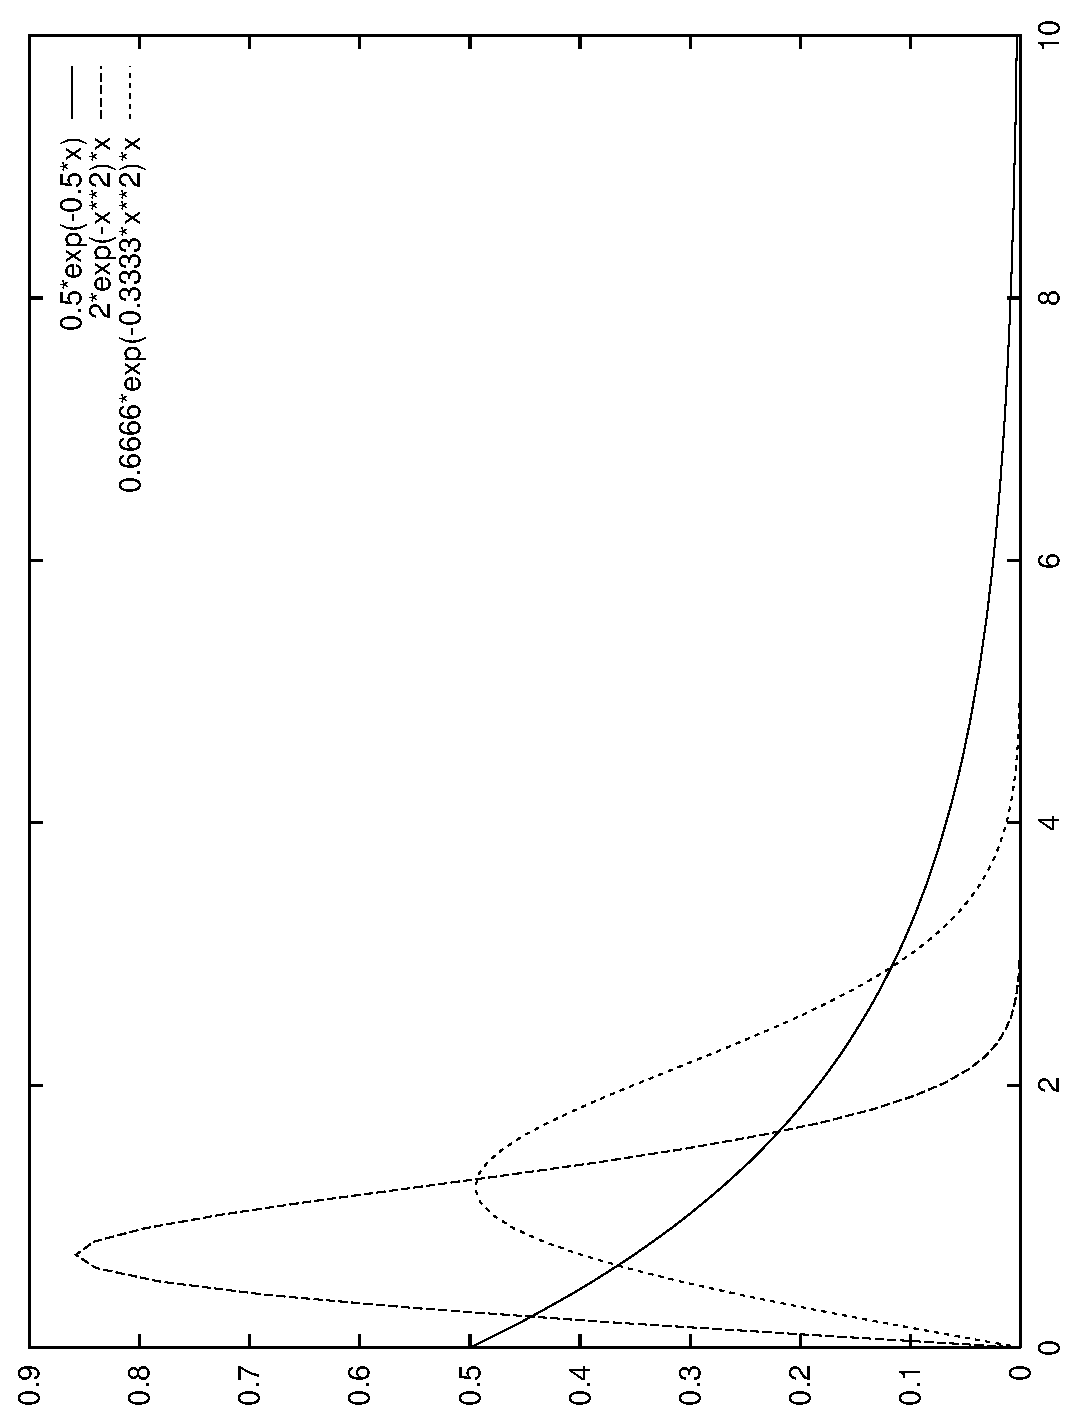
\includegraphics[height=12cm]{weibull.eps}}\\
\caption{The Weibull distribution $(\alpha ,\beta
)=(1,2),(2,1),(2,3)$.}
\end{figure}
\end{center}

\clearpage

\section{Internal Variables}

\begin{itemize}
\item pAlpha - The constant variable $\alpha$.
\item pBeta - The constant variable $\beta$.
\end{itemize}

%********************
\index{pAlpha (Variable)}
\index{pBeta (Variable)}
%********************

\vspace*{10mm}

\section{Public Methods}

\noindent
These methods can be used by all \cpp - programs, that have included the
header file Weibull.h and the library EA. If you declare only
Population.h, we can't use these methods in this version.

\subsection{Constructors}

%---------------------------------------------------------------------------%
% 001
\index{Weibull!( double alpha, double beta )}
\setNormalInstance
\setCorrectWidthThree{8pt}
\setParamOne{alpha}{double}{The constant variable $\alpha$.} 
\setParamTwo{beta}{double}{The constant variable $\beta$.}
\printMethodWithParamsSaved
{}
{None.}
{Weibull}
{The default constructor. Generates the random generator of Weibull distribution.}
{None.}
\setCorrectWidthThree{4pt}
%---------------------------------------------------------------------------%

%---------------------------------------------------------------------------%
% 002
\index{Weibull!( double alpha, double beta, RNG\& rng )}
\setNormalInstance
\setCorrectWidthThree{8pt}
\setParamOne{alpha}{double}{The constant variable $\alpha$.} 
\setParamTwo{beta}{double}{The constant variable $\beta$.}
\setParamThree{rng}{RNG\&}{RNG class.}
\printMethodWithParamsSaved
{}
{None.}
{Weibull}
{The constructor. Generates the random generator of Weibull distribution.}
{None.}
\setCorrectWidthThree{4pt}
%---------------------------------------------------------------------------%

\clearpage

\subsection{Operators}

%---------------------------------------------------------------------------%
% 003
\index{operator( )!( double alpha, double beta )}
\setNormalInstance
\setCorrectWidthThree{8pt}
\setParamOne{alpha}{double}{The constant variable $\alpha$.} 
\setParamTwo{beta}{double}{The constant variable $\beta$.}
\printMethodWithParamsSaved
{double}
{The result of Weibull distribution.}
{operator( )}
{Gets the result of Weibull distribution.}
{None.}
\setCorrectWidthThree{4pt}
%---------------------------------------------------------------------------%

%---------------------------------------------------------------------------%
% 004
\index{operator( )!( )} 
\setNormalInstance
\printEmptyMethodReturnSpecial
{double}
{operator( )}
{Gets the result of Weibull distribution.}
{The result of Weibull distribution.}
{None.}
%---------------------------------------------------------------------------%

\vspace*{10mm}

\subsection{Information Retrieval Methods}

%---------------------------------------------------------------------------%
% 005
\index{alpha!( )} 
\setConstInstance
\printEmptyMethodReturnSpecial
{double}
{alpha}
{Returns the constant variable {\em pAlpha}.}
{The constant variable {\em pAlpha}.}
{None.}
%---------------------------------------------------------------------------%

%---------------------------------------------------------------------------%
% 006
\index{beta!( )} 
\setConstInstance
\printEmptyMethodReturnSpecial
{double}
{beta}
{Returns the constant variable {\em pBeta}.}
{The constant variable {\em pBeta}.}
{None.}
%---------------------------------------------------------------------------%

\clearpage

%---------------------------------------------------------------------------%
% 007
\index{alpha!( double a )} 
\setNormalInstance
\printMethodWithOneParam
{void}
{aplha}
{double}
{a}
{New value of the constant variable {\em pAlpha}.}
{Sets the variable {\em pAlpha} using new variable {\em a}.}
{None.}
{None.}
%---------------------------------------------------------------------------%

%---------------------------------------------------------------------------%
% 008
\index{beta!( double b )} 
\setNormalInstance
\printMethodWithOneParam
{void}
{beta}
{double}
{b}
{New value of the constant variable {\em pBeta}.}
{Sets the variable {\em pBeta} using new variable {\em b}.}
{None.}
{None.}
%---------------------------------------------------------------------------%

\vspace*{10mm}

\subsection{The probability}

%---------------------------------------------------------------------------%
% 010
\index{p!( const double\& x )} 
\setConstInstance
\printMethodWithOneParam
{double}
{p}
{const double\&}
{x}
{The factor which you want to calculate the probability.}
{Returns the probability of {\em x}.}
{The probability.}
{None.}
%---------------------------------------------------------------------------%
















%************************************************************************
% Appendix
%************************************************************************
\clearpage
\chapter*{Appendix A. Sample Programs and Results}
\addcontentsline{toc}{chapter}{Appendix A. Sample Programs and Results}
\index{Sample Programs and Results}
\noindent
{\Large A-2. Random Generators}
\addcontentsline{toc}{section}{A-2. Random Generators}

\vspace*{7mm}

\noindent
In this section, I will explain how to generate random numbers. I
prepared five sample programs for the Cauchy distribution, Log Normal
distribution, Normal distribution, Uniform distribution and
Weibull distribution. 

\vspace*{20mm}

\noindent
{\Large A-2-1. Sample Program 6 (Cauchy)}
\addcontentsline{toc}{subsection}{A-2-1. Sample Program 6}
\index{Cauchy}

\vspace*{7mm}

\noindent
The equation for the Cauchy distribution is as follows.

\begin{equation}
f(x) = \frac{1}{\pi} \cdot \frac{1}{1+x^2}
\end{equation}

\noindent
The next program is a sample for the Cauchy distribution.

\vspace*{10mm}

{\footnotesize
\begin{center}
\begin{tabular}{|l|}\hline
\#include "Population.h"\\
\#include $<$fstream.h$>$\\
\#include $<$stdio.h$>$\\
\hspace*{\textwidth}\\
void main(void)\\
\{\\
\hspace*{10mm}// declaration\\
\hspace*{10mm}int seed      = 1234;\\
\hspace*{10mm}int i,j;\\
\hspace*{10mm}int total     = 1000000;\\
\hspace*{10mm}double r;\\
\hspace*{10mm}double rstore[total];\\
\hspace*{10mm}double start  = -50.05;\\
\hspace*{10mm}double end    =  50.05;\\
\hspace*{10mm}int div       =   1001;\\
\hspace*{10mm}double step   = (end-start)/div;\\
\hspace*{10mm}int counter[div];\\
\hspace*{10mm}double position[div];\\\hline
\end{tabular}
\vspace*{5mm}

{\small
Example 6. Sample Program 6-1.
}
\end{center}
}

\clearpage

{\footnotesize
\begin{center}
\begin{tabular}{|l|}\hline
\hspace*{10mm}// initialization\\
\hspace*{10mm}for (i=0;i$<$div;i++)\{\\
\hspace*{20mm}counter[i]=0;\\
\hspace*{10mm}\}\\
\\
\hspace*{10mm}// file open\\
\hspace*{10mm}FILE *fp;\\
\hspace*{10mm}fp = fopen("data.txt","w");\\
\\
\hspace*{10mm}// random seed\\
\hspace*{10mm}Rng::seed(seed);\\
\\
\hspace*{10mm}// random generator\\
\hspace*{10mm}for (i=0;i$<$total;i++)\{\\
\hspace*{20mm}r = Rng::cauchy();\\
\hspace*{20mm}rstore[i]=r;\\
\hspace*{20mm}for (j=0;j$<$div;j++)\{\\
\hspace*{30mm}position[j] = start + (j+j+1)*step/2.0;\\
\hspace*{30mm}if (r$>$=start+j*step \&\& r$<$start+(j+1)*step)\{\\
\hspace*{40mm}++counter[j];\\
\hspace*{30mm}\}\\
\hspace*{20mm}\}\\
\hspace*{10mm}\}\\
\\
\hspace*{10mm}// output\\
\hspace*{10mm}double prob;\\
\hspace*{10mm}for (j=0;j$<$div;j++)\{\\
\hspace*{20mm}prob = static\_cast$<$double$>$(counter[j]) / static\_cast$<$double$>$(total)/step;\\
\hspace*{20mm}fprintf(fp,"\%f \%f $\backslash$n",position[j],prob);\\
\hspace*{10mm}\}\\
\hspace*{\textwidth}\\
\}\\\hline
\end{tabular}
\vspace*{5mm}

{\small
Example 6. Sample Program 6-2.
}
\end{center}
}

\vspace*{10mm}

\noindent
The result of this program is shown in the next figure.

\clearpage

\begin{center}
\rotatebox{-90}{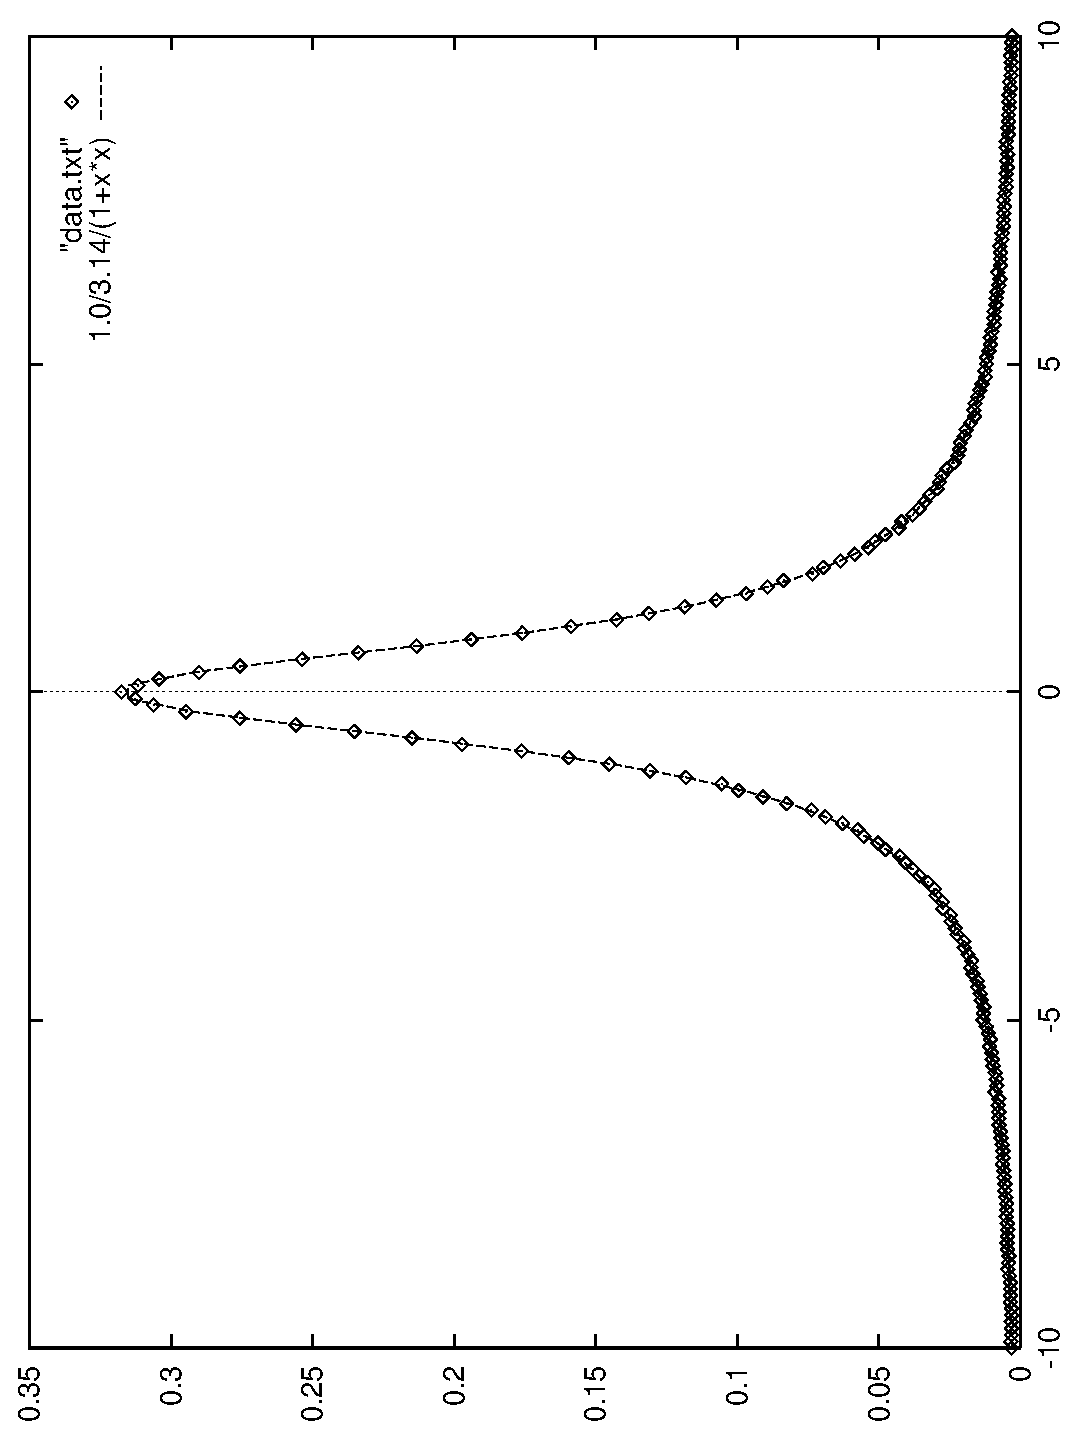
\includegraphics[height=12cm]{i-result-cauchy.eps}}\\
\vspace*{10mm}
Fig. A-2-1. The Cauchy distribution.\\
\end{center}

\vspace*{20mm}

\noindent
{\Large A-2-2. Sample Program 7 (Log Normal)}
\addcontentsline{toc}{subsection}{A-2-2. Sample Program 7}
\index{LogNormal}

\vspace*{7mm}

\noindent
The equation for the Log Normal distribution is as follows.

\begin{equation}
f(x) = \left\{
\begin{array}{ll}
\frac{1}{\sqrt{2\pi} \sigma x} \cdot \exp \left\{ \frac{-(\log x - \mu )^2}{2 \sigma^2} \right\} & x>0 \\
0 & x \le 0
\end{array}
\right.
\end{equation}

\noindent
Here,

\begin{equation}
\mu = \log \left( \frac{\mu_{log}^2}{\sqrt{\mu_{log}^2 +
\sigma_{log}^2}} \right)
\end{equation}

\begin{equation}
\sigma = \sqrt{\log \left( \frac{\mu_{log}^2+\sigma_{log}^2}{\mu_{log}^2} \right)}
\end{equation}

\noindent
In the program, I used 

\begin{equation}
\mu_{log} = \sqrt{e}
\end{equation}

\clearpage

\begin{equation}
\sigma_{log}^2 = e (e-1)
\end{equation}

\vspace*{5mm}

\noindent
The next program is a sample for the Log Normal distribution.

\vspace*{10mm}

{\footnotesize
\begin{center}
\begin{tabular}{|l|}\hline
\#include "Population.h"\\
\#include $<$fstream.h$>$\\
\#include $<$stdio.h$>$\\
\#include $<$LogNormal.h$>$\\
\hspace*{\textwidth}\\
void main(void)\\
\{\\
\\
\hspace*{10mm}// declaration\\
\hspace*{10mm}int seed      = 1234;\\
\hspace*{10mm}int i,j;\\
\hspace*{10mm}int total     = 1000000;\\
\hspace*{10mm}double r;\\
\hspace*{10mm}double rstore[total];\\
\hspace*{10mm}double start  = -0.005;\\
\hspace*{10mm}double end    = 10.005;\\
\hspace*{10mm}int div       =   1001;\\
\hspace*{10mm}double step   = (end-start)/div;\\
\hspace*{10mm}int counter[div];\\
\hspace*{10mm}double position[div];\\
\\
\hspace*{10mm}// instantialize\\
\hspace*{10mm}LogNormal lognormal;\\
\\
\hspace*{10mm}// initialization\\
\hspace*{10mm}for (i=0;i$<$div;i++)\{\\
\hspace*{20mm}counter[i]=0;\\
\hspace*{10mm}\}\\
\\
\hspace*{10mm}// file open\\
\hspace*{10mm}FILE *fp;\\
\hspace*{10mm}fp = fopen("data.txt","w");\\
\\
\hspace*{10mm}// random seed\\
\hspace*{10mm}Rng::seed(seed);\\\hline
\end{tabular}
\vspace*{5mm}

{\small
Example 7. Sample Program 7-1.
}
\end{center}
}

\clearpage

{\footnotesize
\begin{center}
\begin{tabular}{|l|}\hline
\hspace*{10mm}// random generator\\
\hspace*{10mm}for (i=0;i$<$total;i++)\{\\
\hspace*{20mm}lognormal.mean(SqrtE);\\
\hspace*{20mm}lognormal.variance(E*(E-1));\\
\hspace*{20mm}r = lognormal();\\
\hspace*{20mm}rstore[i]=r;\\
\hspace*{20mm}for (j=0;j$<$div;j++)\{\\
\hspace*{30mm}position[j] = start + (j+j+1)*step/2.0;\\
\hspace*{30mm}if (r$>$=start+j*step \&\& r<start+(j+1)*step)\{\\
\hspace*{40mm}++counter[j];\\
\hspace*{30mm}\}\\
\hspace*{20mm}\}\\
\hspace*{10mm}\}\\
\\
\hspace*{10mm}// output\\
\hspace*{10mm}double prob;\\
\hspace*{10mm}for (j=0;j$<$div;j++)\{\\
\hspace*{20mm}prob = static\_cast$<$double$>$(counter[j]) / static\_cast$<$double$>$(total)/step;\\
\hspace*{20mm}fprintf(fp,"\%f \%f $\backslash$n",position[j],prob);\\
\hspace*{10mm}\}\\
\hspace*{\textwidth}\\
\}\\\hline
\end{tabular}
\vspace*{5mm}

{\small
Example 7. Sample Program 7-2.
}
\end{center}
}

\vspace*{10mm}

\noindent
The result of this program is shown in the next figure.

\clearpage

\begin{center}
\rotatebox{-90}{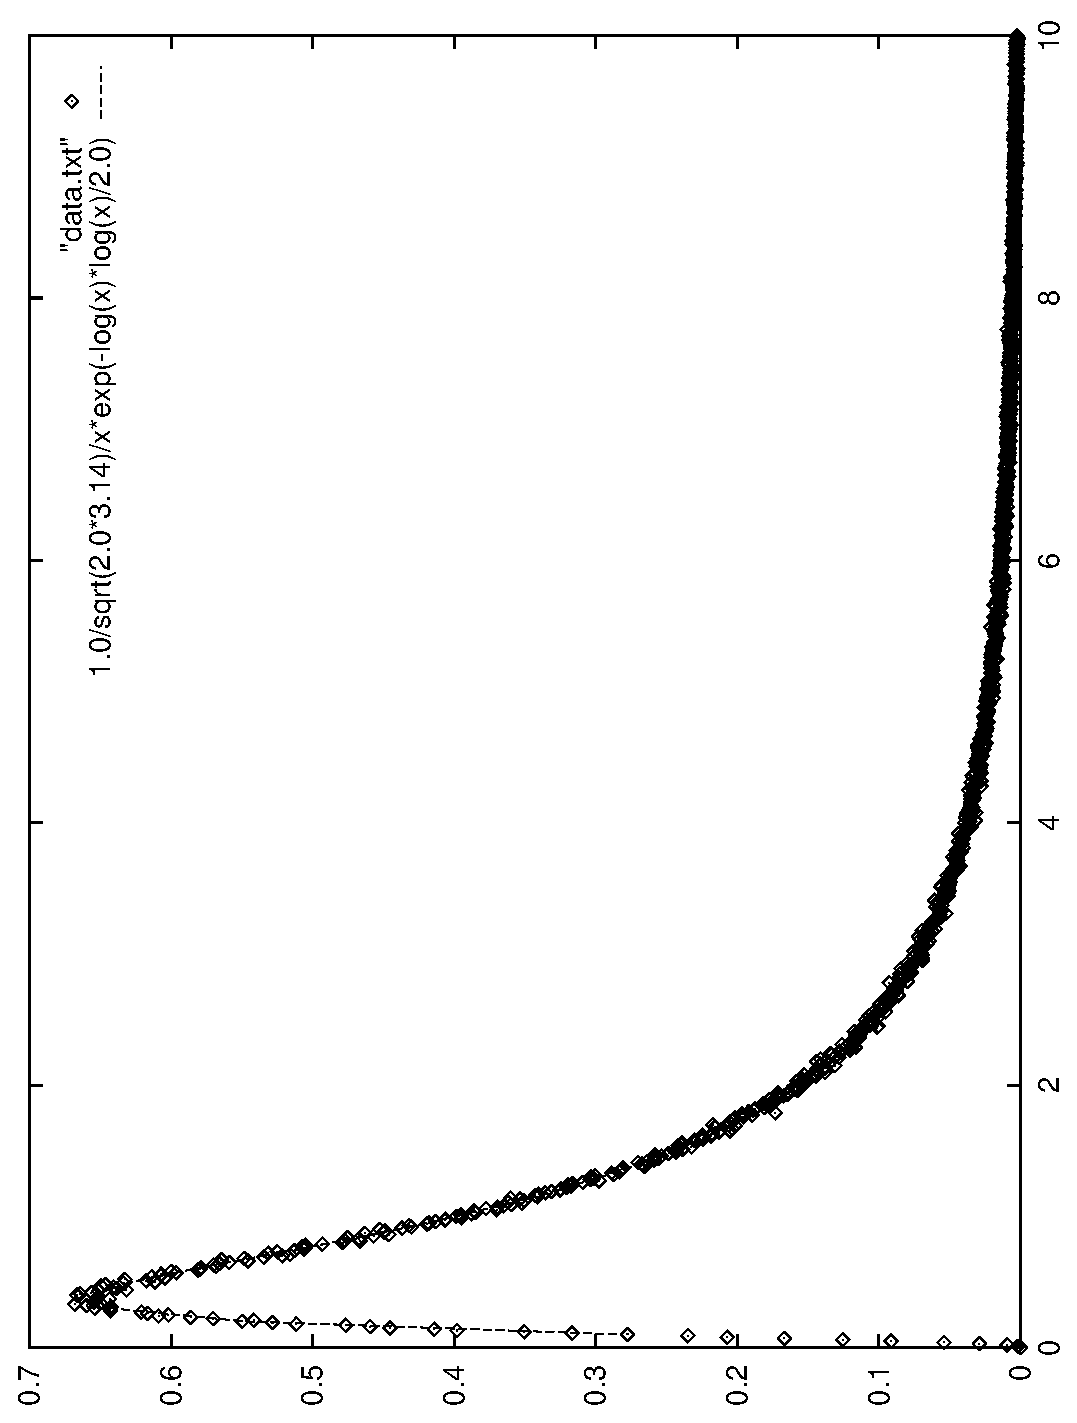
\includegraphics[height=12cm]{i-result-lognormal.eps}}\\
\vspace*{10mm}
Fig. A-2-2. The Log Normal distribution.\\
\end{center}

\vspace*{20mm}

\noindent
{\Large A-2-3. Sample Program 8 (Normal)}
\addcontentsline{toc}{subsection}{A-2-3. Sample Program 8}
\index{Normal}

\vspace*{7mm}

\noindent
The equation for the Normal distribution is as follows.

\begin{equation}
f(x) = \frac{1}{\sqrt{2\pi}\sigma} \cdot \exp{\frac{-(x-\mu)^2}{2\sigma^2}}
\end{equation}

\noindent
In the program, I used

\begin{equation}
\mu = 3 \hspace{3mm} , \hspace{3mm} \sigma^2 = 4
\end{equation}

\vspace*{5mm}

\noindent
The next program is a sample for the Normal distribution.

\clearpage

{\footnotesize
\begin{center}
\begin{tabular}{|l|}\hline
\#include "Population.h"\\
\#include $<$fstream.h$>$\\
\#include $<$stdio.h$>$\\
\hspace*{\textwidth}\\
void main(void)\\
\{\\
\\
\hspace*{10mm}// declaration\\
\hspace*{10mm}int seed      = 1234;\\
\hspace*{10mm}int i,j;\\
\hspace*{10mm}int total     = 1000000;\\
\hspace*{10mm}double r;\\
\hspace*{10mm}double rstore[total];\\
\hspace*{10mm}double start  = -3.006;\\
\hspace*{10mm}double end    =  9.006;\\
\hspace*{10mm}int div       =   1001;\\
\hspace*{10mm}double step   = (end-start)/div;\\
\hspace*{10mm}int counter[div];\\
\hspace*{10mm}double position[div];\\
\\
\hspace*{10mm}// initialization\\
\hspace*{10mm}for (i=0;i$<$div;i++)\{\\
\hspace*{20mm}counter[i]=0;\\
\hspace*{10mm}\}\\
\\
\hspace*{10mm}// file open\\
\hspace*{10mm}FILE *fp;\\
\hspace*{10mm}fp = fopen("data.txt","w");\\
\\
\hspace*{10mm}// random seed\\
\hspace*{10mm}Rng::seed(seed);\\
\\
\hspace*{10mm}// random generator\\
\hspace*{10mm}for (i=0;i$<$total;i++)\{\\
\hspace*{20mm}Rng::gauss.mean(3.0);\\
\hspace*{20mm}Rng::gauss.variance(4.0);\\
\hspace*{20mm}r = Rng::gauss();\\
\hspace*{20mm}rstore[i]=r;\\
\hspace*{20mm}for (j=0;j$<$div;j++)\{\\
\hspace*{30mm}position[j] = start + (j+j+1)*step/2.0;\\
\hspace*{30mm}if (r$>$=start+j*step \&\& r<start+(j+1)*step)\{\\
\hspace*{40mm}++counter[j];\\
\hspace*{30mm}\}\\
\hspace*{20mm}\}\\
\hspace*{10mm}\}\\\hline
\end{tabular}
\vspace*{5mm}

{\small
Example 8. Sample Program 8-1.
}
\end{center}
}

\clearpage

{\footnotesize
\begin{center}
\begin{tabular}{|l|}\hline
\hspace*{10mm}// output\\
\hspace*{10mm}double prob;\\
\hspace*{10mm}for (j=0;j$<$div;j++)\{\\
\hspace*{20mm}prob = static\_cast$<$double$>$(counter[j]) / static\_cast$<$double$>$(total)/step;\\
\hspace*{20mm}fprintf(fp,"\%f \%f $\backslash$n",position[j],prob);\\
\hspace*{10mm}\}\\
\hspace*{\textwidth}\\
\}\\\hline
\end{tabular}
\vspace*{5mm}

{\small
Example 8. Sample Program 8-2.
}
\end{center}
}

\vspace*{10mm}

\noindent
The result of this program is shown in the next figure.

\vspace*{10mm}

\begin{center}
\rotatebox{-90}{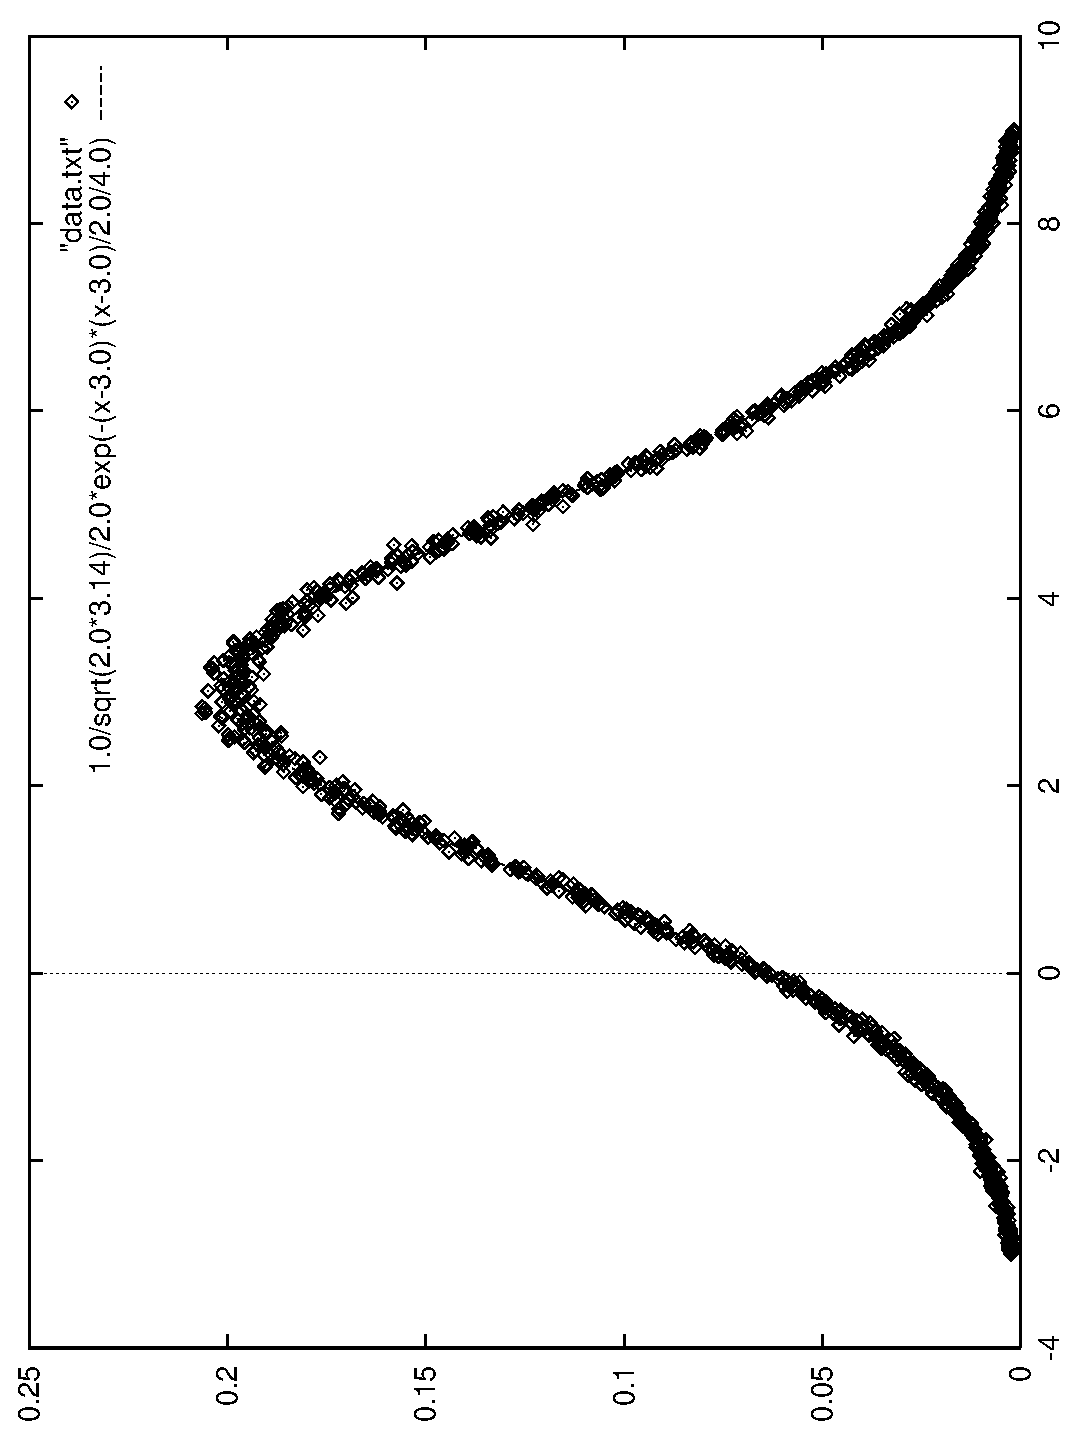
\includegraphics[height=12cm]{i-result-normal.eps}}\\
\vspace*{10mm}
Fig. A-2-3. The Normal distribution.\\
\end{center}

\clearpage

\noindent
{\Large A-2-4. Sample Program 9 (Uniform)}
\addcontentsline{toc}{subsection}{A-2-4. Sample Program 9}
\index{Uniform}

\vspace*{7mm}

\noindent
The equation for the Uniform distribution is as follows.

\begin{equation}
f(x) = \left\{
\begin{array}{ll}
1 / ( x_{upper} - x_{lower} )  & x_{lower} \le x \le x_{upper} \\
0 & the \hspace{2mm} other
\end{array}
\right.
\end{equation}

\noindent
In the program, I used

\begin{equation}
x_{lower} = 1.0 \hspace{3mm} , \hspace{3mm} x_{upper} = 2.0
\end{equation}

\vspace*{5mm}

\noindent
The next program is a sample for the Uniform distribution.

\vspace*{10mm}

{\footnotesize
\begin{center}
\begin{tabular}{|l|}\hline
\#include "Population.h"\\
\#include $<$fstream.h$>$\\
\#include $<$stdio.h$>$\\
\hspace*{\textwidth}\\
void main(void)\\
\{\\
\\
\hspace*{10mm}// declaration\\
\hspace*{10mm}int seed      = 1234;\\
\hspace*{10mm}int i,j;\\
\hspace*{10mm}int total     = 1000000;\\
\hspace*{10mm}double r;\\
\hspace*{10mm}double rstore[total];\\
\hspace*{10mm}double start  = 1.0;\\
\hspace*{10mm}double end    = 2.0;\\
\hspace*{10mm}int div       = 1000;\\
\hspace*{10mm}double step   = (end-start)/div;\\
\hspace*{10mm}int counter[div];\\
\hspace*{10mm}double position[div];\\
\\
\hspace*{10mm}// initialization\\
\hspace*{10mm}for (i=0;i$<$div;i++)\{\\
\hspace*{20mm}counter[i]=0;\\
\hspace*{10mm}\}\\\hline
\end{tabular}
\vspace*{5mm}

{\small
Example 9. Sample Program 9-1.
}
\end{center}
}  

\clearpage

{\footnotesize
\begin{center}
\begin{tabular}{|l|}\hline
\hspace*{10mm}// file open\\
\hspace*{10mm}FILE *fp;\\
\hspace*{10mm}fp = fopen("data.txt","w");\\
\\
\hspace*{10mm}// random seed\\
\hspace*{10mm}Rng::seed(seed);\\
\\
\hspace*{10mm}// random generator\\
\hspace*{10mm}for (i=0;i$<$total;i++)\{\\
\hspace*{20mm}Rng::uni.low(start);\\
\hspace*{20mm}Rng::uni.high(end);\\
\hspace*{20mm}r = Rng::uni();\\
\hspace*{20mm}rstore[i]=r;\\
\hspace*{20mm}for (j=0;j$<$div;j++)\{\\
\hspace*{30mm}position[j] = start + (j+j+1)*step/2.0;\\
\hspace*{30mm}if (r$>$=start+j*step \&\& r<start+(j+1)*step)\{\\
\hspace*{40mm}++counter[j];\\
\hspace*{30mm}\}\\
\hspace*{20mm}\}\\
\hspace*{10mm}\}\\
\\
\hspace*{10mm}// output\\
\hspace*{10mm}double prob;\\
\hspace*{10mm}for (j=0;j$<$div;j++)\{\\
\hspace*{20mm}prob = static\_cast$<$double$>$(counter[j]) / static\_cast$<$double$>$(total)/step;\\
\hspace*{20mm}fprintf(fp,"\%f \%f $\backslash$n",position[j],prob);\\
\hspace*{10mm}\}\\
\\
\}\\\hline
\end{tabular}
\vspace*{5mm}

{\small
Example 9. Sample Program 9-2.
}
\end{center}
}  

\vspace*{5mm}

\noindent
The result of this program is shown in the next figure.

\clearpage

\begin{center}
\rotatebox{-90}{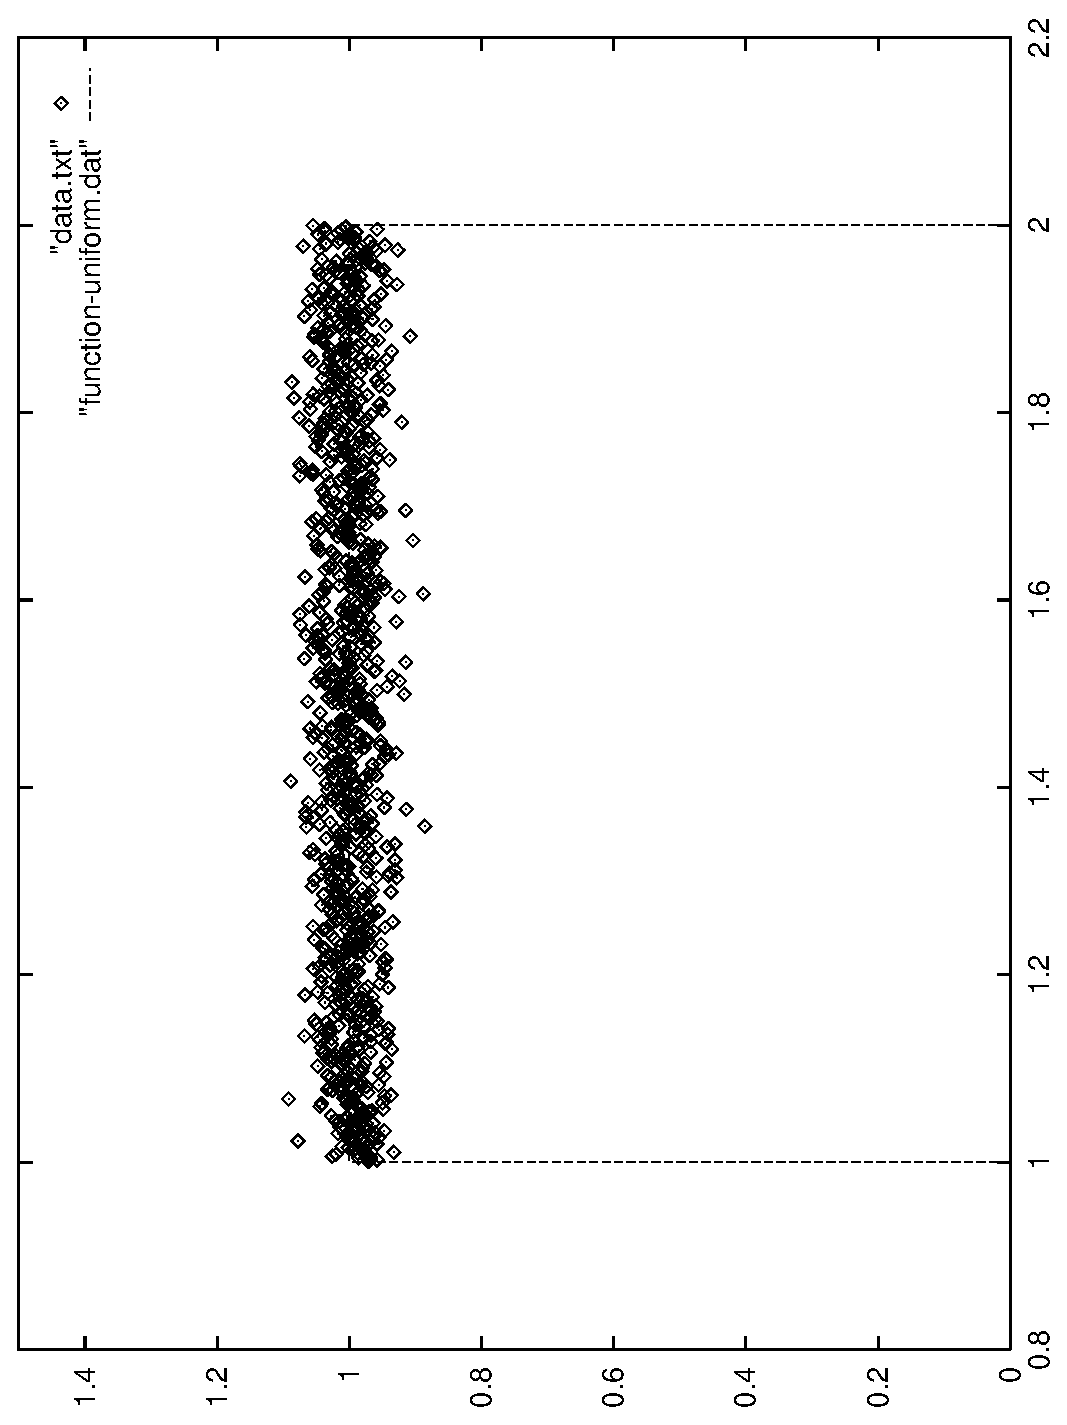
\includegraphics[height=12cm]{i-result-uniform.eps}}\\
\vspace*{10mm}
Fig. A-2-4. The Uniform distribution.\\
\end{center}

\vspace*{20mm}

\noindent
{\Large A-2-5. Sample Program 10 (Weibull)}
\addcontentsline{toc}{subsection}{A-2-5. Sample Program 10}
\index{Weibull}

\vspace*{7mm}

\noindent
The equation for the Weibull distribution is as follows.

\begin{equation}
f(x) = \frac{\alpha}{\beta} \cdot \exp \left\{ - \frac{1}{\beta} x^\alpha \right\} \cdot x^{\alpha-1}
\end{equation}

\noindent
In the program, I used

\begin{equation}
\alpha = 2  \hspace{3mm} , \hspace{3mm} \beta = 3
\end{equation}

\vspace*{5mm}

\noindent
The next program is a sample for the Weibull distribution.

\clearpage

{\footnotesize
\begin{center}
\begin{tabular}{|l|}\hline
\#include "Population.h"\\
\#include $<$fstream.h$>$\\
\#include $<$stdio.h$>$\\
\#include $<$Weibull.h$>$\\
\hspace*{\textwidth}\\
void main(void)\\
\{\\
\\
\hspace*{10mm}// declaration\\
\hspace*{10mm}int seed      = 1234;\\
\hspace*{10mm}int i,j;\\
\hspace*{10mm}int total     = 1000000;\\
\hspace*{10mm}double r;\\
\hspace*{10mm}double rstore[total];\\
\hspace*{10mm}double start  = -0.005;\\
\hspace*{10mm}double end    = 10.005;\\
\hspace*{10mm}int div       = 1001;\\
\hspace*{10mm}double step   = (end-start)/div;\\
\hspace*{10mm}int counter[div];\\
\hspace*{10mm}double position[div];\\
\\
\hspace*{10mm}// instantialize\\
\hspace*{10mm}Weibull weibull;\\
\\
\hspace*{10mm}// initialization\\
\hspace*{10mm}for (i=0;i$<$div;i++)\{\\
\hspace*{20mm}counter[i]=0;\\
\hspace*{10mm}\}\\
\\
\hspace*{10mm}// file open\\
\hspace*{10mm}FILE *fp;\\
\hspace*{10mm}fp = fopen("data.txt","w");\\
\\
\hspace*{10mm}// random seed\\
\hspace*{10mm}Rng::seed(seed);\\
\hspace*{10mm}// random generator\\
\hspace*{10mm}for (i=0;i$<$total;i++)\{\\
\hspace*{20mm}weibull.alpha(2.0);\\
\hspace*{20mm}weibull.beta(3.0);\\
\hspace*{20mm}r = weibull();\\
\hspace*{20mm}rstore[i]=r;\\
\hspace*{20mm}for (j=0;j$<$div;j++)\{\\
\hspace*{30mm}position[j] = start + (j+j+1)*step/2.0;\\
\hspace*{30mm}if (r$>$=start+j*step \&\& r$<$start+(j+1)*step)\{\\
\hspace*{40mm}++counter[j];\\\hline
\end{tabular}
\vspace*{5mm}

{\small
Example 10. Sample Program 10-1.
}
\end{center}
}  

\clearpage

  
{\footnotesize
\begin{center}
\begin{tabular}{|l|}\hline

\hspace*{30mm}\}\\
\hspace*{20mm}\}\\
\hspace*{10mm}\}\\
\\
\hspace*{10mm}// output\\
\hspace*{10mm}double prob;\\
\hspace*{10mm}for (j=0;j$<$div;j++)\{\\
\hspace*{20mm}prob = static\_cast$<$double$>$(counter[j]) / static\_cast$<$double$>$(total)/step;\\
\hspace*{20mm}fprintf(fp,"\%f \%f $\backslash$n",position[j],prob);\\
\hspace*{10mm}\}\\
\hspace*{\textwidth}\\
\}\\\hline
\end{tabular}
\vspace*{5mm}

{\small
Example 10. Sample Program 10-2.
}
\end{center}
}  
  
\vspace*{5mm}

\noindent
The result of this program is shown in the next figure.

\vspace*{5mm}

\begin{center}
\rotatebox{-90}{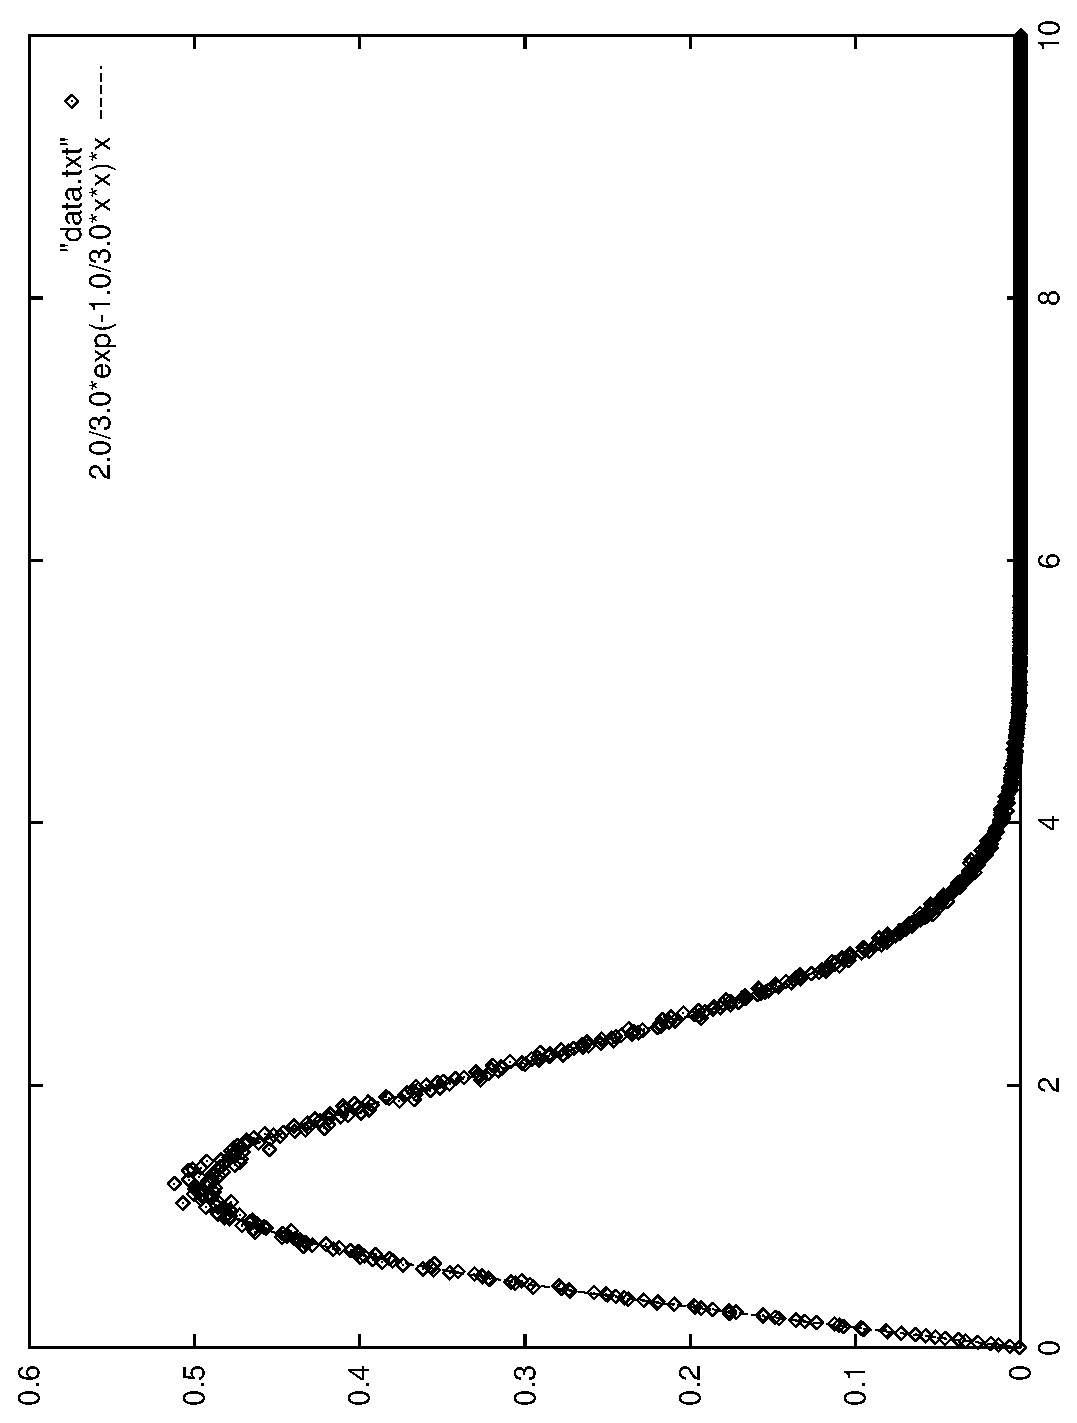
\includegraphics[height=12cm]{i-result-weibull.eps}}\\
\vspace*{10mm}
Fig. A-2-5. Weibull distribution.\\
\end{center}







%************************************************************************
% Bibliography
%************************************************************************
\clearpage
\addcontentsline{toc}{chapter}{Bibliography}
\begin{thebibliography}{55}
 
    \bibitem{Foundations}
    {\em Foundations of Genetic Algorithms}, G.J.E. Rawlings (Editor),
    Morgan Kaufmann Publishers, San Mateo, CA, 1991.

    \bibitem{ICEC96}
    {\em Proceedings of the 1996 IEEE Internal Conference on Evolutionary 
    Computation (ICEC '96)}.
   
    \bibitem{First}
    {\em Proceedings of the First International Conference on Genetic 
    Algorithms and Their Applications} (ICGA 1985), published by
    J.J. Grefenstette, Pittsburgh, PA, Juli 24-26 1985, Carnegie-Mellon 
    University, Lawrence Erlbaum Associates (Hillsdale, NJ, 1988).

    \bibitem{Third}
    {\em Proceedings of the Third International Conference on Genetic 
    Algorithms} (ICGA 1989), published by J.D. Schaffer, July 4-7, 
    San Mateo, CA, 1989, George Mason University, Morgan Kaufmann 
    Publishers Inc.

    \bibitem{Eshelman95}
    {\em Proceedings of the Sixth International Conference on Genetic
    Algorithms}, published by L.J. Eshelman, 1995.

    \bibitem{Goldberg}
    {\em A comparative analysis of selection schemes used in genetic
    algorithms}, by D.E. Goldberg and K. Deb published at pages
    69 to 93 in \cite{Foundations}.

    \bibitem{Baeck}
    {\em Evolutionary Algorithms in Theory and Practice}, 
    dissertation thesis by T. B\"ack, University of Dortmund, 
    Department of Computer Science, February 1994.

    \bibitem{EALibRef}
    {\em EALib: A \cpp\ class library for evolutionary algorithms}, 
    version 1.5, 2000, by M. Kreutz, B. Sendhoff and C. Igel, 
    Institut f\"ur Neuroinformatik, Ruhr-Universit\"at Bochum.

    \bibitem{Baker}
    {\em Adaptive Selection methods for genetic algorithms}, by J.E. Baker, 
    published at the pages 101 to 111 in \cite{First}.

    \bibitem{AlgoWork}
    {\em How genetic algorithms work: A critical look at implicit
    parallelism}, by J.J. Grefenstette and J.E. Baker, published
    at the pages 20 to 27 in \cite{Third}. 

    \bibitem{Whitley}
    {\em The genitor algorithm and selection pressure:
    Why rank-based allocation of reproductive trials is best} by L.D.
    Whitley, published at the pages 116 to 121 in \cite{Third}.

    \bibitem{Fogel}
    {\em Evolutionary Computation: Toward a New Philosophy of
    Machine Intelligence} by D.B. Fogel, IEEE Press, 1995.

    \bibitem{Search}
    {\em Genetic Algorithms in Search, Optimization, and Machine Learning}, 
    by D.E. Goldberg, Addison-Wesley Publishing Company, Inc., Reading, MA, 
    1989.

    \bibitem{Jong}
    {\em An Analysis of the Behaviour of a Class of Genetic Adaptive
    Systems} by K.A.D. Jong, Dept. Computer and Communication Sciences,
    University of Michigan, 1975, Diss. Abstr. Int. 36(10), 5140B,
    University Microfilms No. 76-9381.

    \bibitem{GSA}
    {\em On the Adaptation of Arbitrary Normal Mutation Distributions
    in Evolution Strategies: The Generating Set Adaptation},
    by N. Hansen, A. Ostermeier and A. Gawelczyk, published at the pages
    57 to 64 in \cite{Eshelman95}. 

    \bibitem{CMA}
    {\em Adapting Arbitrary Normal Mutation. Distributions in Evolution
    Strategies: The Covariance Matrix Adaptation}, by N. Hansen and A. 
    Ostermeier, appeared at the pages 312 to 317 in \cite{ICEC96}.

    \bibitem{MSR}
    {\em Schrittweitenadaptation in der Evolutionsstrategie mit einem
    ent\-sto\-chasti\-sier\-ten Ansatz}, by A. Ostermeier, dissertation thesis, 
    Technische Universit\"at Berlin, Fachbereich 6, 1997.

    \bibitem{NRC}
    {\em Numerical Recipes in C ( Second Edition )}, by William
    H. Press, Saul A. Teukolsky, William T. Vettering and Brian
    P. Flannery, Cambridge University Press, 1992. \label{NRC}

\end{thebibliography}



%************************************************************************
% Index
%************************************************************************
\clearpage
\printindex{}


\end{document}






